% concatenated from Draft4_2025.10.10_arxiv.tex
\documentclass[12pt,reqno]{amsart}
\usepackage{amsmath,amssymb,amsthm,amscd}
%\usepackage{mathtools}
\usepackage{mathrsfs}
\usepackage[old]{old-arrows} 
\usepackage{stmaryrd}% this package enables the use of an inverted mapsto symbol, i.e., \mapsfrom

\usepackage[utf8]{inputenc}
\usepackage[english]{babel}

\usepackage{tikz}
\usepackage{tikz-cd}%to draw commutative diagrams
\usetikzlibrary{babel} %to avoid trouble when labeling arrows in commutative diagrams
\usetikzlibrary{cd} %to get hook arrows with the hook upside down; to get this write hook'
\tikzset{
  symbol/.style={
    draw=none,
    every to/.append style={
      edge node={node [sloped, allow upside down,
      auto=false]{$#1$}}}
  }
}% this code makes it possible to write inclusion symbols instead of injection arrows (\ar[..,hook]) in commutative diagrams; write \ar[u,symbol=\subseteq] or \ar[u,symbol=\superseteq] to get the desired symbol



%\usepackage{fancyhdr}
\usepackage{graphicx}
\usepackage[alphabetic]{amsrefs}
%\usepackage[colorlinks, citecolor=blue, backref=page]{hyperref}
\usepackage[bookmarks=false,hypertexnames=false,colorlinks, citecolor=blue]{hyperref}
\usepackage{bookmark}
\usepackage{verbatim,color,geometry}
\geometry{a4paper,top=3.5cm,bottom=3.8cm,left=2.5cm,right=2.5cm}
\usepackage{marginnote}
\usepackage[colorinlistoftodos, textsize=small]{todonotes}
%to write notes in the text; just write \todo{.......}
\setlength\marginparwidth{0.7in} %this solves the todonotes problem in the amsart package

\newcommand{\todoo}[2][]{\todo[size=tiny, #1]{#2}} %% my notes
\newcommand{\toda}[2][]{\todo[color=blue!30, #1]{#2}} %% my notes
\newcommand{\tode}[2][]{\todo[color=green!50, #1]{#2}} % notes for Karl 1
\newcommand{\todee}[2][]{\todo[color=yellow, #1]{#2}} % notes for Karl 2


\makeatletter 
\@mparswitchfalse%
\makeatother
\reversemarginpar
%write \normalmarginpar for right-handed notes and lines, or 
%\reversemarginpar %if you want them on the left of your twosided document. 
%%%%% to have todonotes on one side of the page only (left or right)

\usepackage[shortlabels]{enumitem} % shortlabels enables to write \begin{enumerate}[i.] or [a.], or [A.], or [(1)] etc. to get the desired item counter formats
% in the Spanish babel package it is NOT allowed to use lowercase Roman numerals, so when one writes \begin{enumerate}[(i)] the counters (I),(II),... are shown
% use [\normalfont (i)] or [\upshape (i)] to get non-italized counters
% use [\bfseries (R\arabic*).] to get item counters (r_1)., (R2)., etc.
%\setcounter{tocdepth}{1}


%\numberwithin{equation}{section}

\newtheorem{thm}{Theorem}[section]
\newtheorem{prop}[thm]{Proposition}
\newtheorem{defn-thm}[thm]{Theorem-Definition}
\newtheorem{defn-lem}[thm]{Lemma-Definition}
\newtheorem{cor}[thm]{Corollary}
\newtheorem{conj}[thm]{Conjecture}
\newtheorem{lem}[thm]{Lemma}
\newtheorem*{thm*}{Theorem}
\newtheorem*{prop*}{Proposition}
\newtheorem*{cor*}{Corollary}
\newtheorem*{lem*}{Lemma}

\theoremstyle{definition}
\newtheorem{que}[thm]{Question}
\newtheorem{defn}[thm]{Definition}
\newtheorem{example}[thm]{Example}
\newtheorem{rem}[thm]{Remark}
%\newtheorem{rem}[thm]{\it Remark}
\newtheorem{claim}[thm]{Claim}
\newtheorem{notation}[thm]{Notation}
\newtheorem*{ans}{Answer}
\newtheorem*{conv}{Convention}
\newtheorem*{mthm}{Main Theorem}
\newtheorem*{claim*}{Claim}
\newtheorem*{rem*}{Remark}

\newcommand{\note}[1]{\textcolor{red}{#1}}

%%% code to abbreviate constants m_0,n_1
%\newcommand{\aO}{a_2}  %% ancient (Original) a
%\newcommand{\bO}{a_1}  %% ancient (Original) b
%\newcommand{\cO}{a_0}  %% ancient (Original) c
%\newcommand{\aA}{a_0}  %% new a_0
%\newcommand{\aB}{a_1}  %% new a_1
%\newcommand{\aC}{a_2}  %% new a_2
%\newcommand{\bA}{b_0}  %% ancient b_0
%\newcommand{\bB}{b_1}  %% ancient b_1
%\newcommand{\bC}{b_2}  %% ancient b_2
%\newcommand{\cA}{b_3}  %% ancient c_0
%\newcommand{\cB}{b_4}  %% ancient c_1
%\newcommand{\mA}{c_0}  %% ancient m_0
%\newcommand{\mB}{c_1}  %% ancient m_1
%\newcommand{\mC}{c_2}  %% ancient m_2
%\newcommand{\nA}{c_3}  %% ancient n_0
%\newcommand{\nB}{c_4}  %% ancient n_1
%\newcommand{\pA}{c_5}  %% ancient p_0
%\newcommand{\pB}{c_6}  %% ancient p_1
%\newcommand{\pC}{c_7}  %% ancient p_2
%\newcommand{\aT}{a}  %% final 'a' in main Theorem
%\newcommand{\cT}{c}  %% final 'c' in main Theorem
%\newcommand{\m}{m_1}  %% final 'm' in main theorem --> it comes from m_1
%\newcommand{\n}{n_0}  %% final 'n' in main theorem --> it comes from n_0
%\newcommand{\wO}{z}  %% ancient variable w
%\newcommand{\zO}{w}  %% ancient variable z



\newcommand{\su}{\subset}
\newcommand{\us}{\supseteq}
\newcommand{\bx}{{\bar{x}}}
\newcommand{\by}{{\bar{y}}}
\newcommand{\bz}{{\bar{z}}}
\newcommand{\bu}{{\bar{u}}}
\newcommand{\bv}{{\bar{v}}}
\newcommand{\bs}{{\bar{s}}}
\newcommand{\bt}{{\bar{t}}}
\newcommand{\hx}{{\hat{x}}}
\newcommand{\hy}{{\hat{y}}}
\newcommand{\hz}{{\hat{z}}}
\newcommand{\ct}{{\breve{t}}}
\newcommand{\cu}{{\breve{u}}}
\newcommand{\cv}{{\breve{v}}}
\newcommand{\cw}{{\breve{w}}}
\newcommand{\cx}{{\breve{x}}}
\newcommand{\cy}{{\breve{y}}}
\newcommand{\cz}{{\breve{z}}}




\newcommand{\then}{\quad\Rightarrow\quad}
\newcommand{\sii}{\quad\Leftrightarrow\quad}
\newcommand{\oto}{\leftrightarrow}
\newcommand{\otto}{\longleftrightarrow}
\newcommand{\ttto}{\dashrightarrow} %arrow for rational maps
\newcommand{\tto}{\longrightarrow}
\newcommand{\ott}{\longleftarrow}
\newcommand{\tosurj}{\twoheadrightarrow}
%\newcommand{\ttosurj}{\longtwoheadrightarrow}
\newcommand{\toinj}{\hookrightarrow}
\newcommand{\ttoinj}{\longhookrightarrow}
\newcommand{\mapstto}{\longmapsto}
\newcommand{\mapsffrom}{\longmapsfrom}
\newcommand{\wt}{\widetilde}
\newcommand{\wh}{\widehat}


\newcommand{\fc}{\displaystyle\frac}
\newcommand{\tf}{\tfrac}
\newcommand{\summm}{\textstyle\sum}
\newcommand{\summ}{\displaystyle\sum}
\newcommand{\ds}{\displaystyle}
\newcommand{\pa}{\partial}
\newcommand{\va}{\emptyset}
\newcommand{\un}{\underline}
\newcommand{\ov}{\overline}
\newcommand{\la}{\langle}
\newcommand{\ra}{\rangle}%\ran in Portuguese
\newcommand{\lf}{\lfloor}%izquierda maximo entero
\newcommand{\rf}{\rfloor}%derecha maximo entero
\newcommand{\ltq}{\preccurlyeq}% less than or equal for equivalence relations
\newcommand{\gtq}{\succcurlyeq}% great than or equal for equivalence relations
\newcommand{\isom}{\cong}% to write isomorphisms
\newcommand{\id}{\text{id}}% to write isomorphisms




\newcommand{\bsymb}{\boldsymbol}


\newcommand{\K}{\mathbb{K}}
\newcommand{\R}{\mathbb{R}}
\newcommand{\N}{\mathbb{N}}
\newcommand{\Z}{\mathbb{Z}}
\newcommand{\Q}{\mathbb{Q}}
\newcommand{\C}{\mathbb{C}}
\newcommand{\PP}{\mathbb{P}}
\newcommand{\E}{\mathbb{E}}
\newcommand{\AAA}{\mathbb{A}}
\newcommand{\F}{\mathbb{F}}
\newcommand{\G}{\mathbb{G}}



\newcommand{\BB}{\mathcal{B}}%%Borel:sets
\newcommand{\CC}{\mathcal{C}}
\newcommand{\DD}{\mathcal{D}}
\newcommand{\EE}{\mathcal{E}}
\newcommand{\FF}{\mathcal{F}}
\newcommand{\GG}{\mathcal{G}}
\newcommand{\HH}{\mathcal{H}}
\newcommand{\II}{\mathcal{I}}
\newcommand{\KK}{\mathcal{K}}
%\newcommand{\AAAA}{\mathcal{A}}
\newcommand{\LL}{\mathcal{L}}
\newcommand{\MM}{\mathcal{M}}%space of prob measure
\newcommand{\OO}{\mathcal{O}}
\newcommand{\PPP}{\mathcal{P}}
\newcommand{\SSS}{\mathcal{S}}
\newcommand{\TT}{\mathcal{T}}
\newcommand{\UU}{\mathcal{U}}
\newcommand{\VV}{\mathcal{V}}
\newcommand{\XX}{\mathcal{X}}




\newcommand{\CCC}{\mathscr{C}}
\newcommand{\DDD}{\mathscr{D}}
\newcommand{\FFF}{\mathscr{F}}


\newcommand{\aaa}{\mathfrak{a}}
\newcommand{\bb}{\mathfrak{b}}
\newcommand{\cc}{\mathfrak{c}}
\newcommand{\dd}{\mathfrak{d}}
\newcommand{\mm}{\mathfrak{m}}
\newcommand{\nn}{\mathfrak{n}}
\newcommand{\pp}{\mathfrak{p}}
\newcommand{\fq}{\mathfrak{q}}
\newcommand{\rr}{\mathfrak{r}}
\newcommand{\s}{\mathfrak{s}}%\ss in Portuguese
\newcommand{\ttt}{\mathfrak{t}}
\newcommand{\NNN}{\mathfrak{N}}
\newcommand{\VVV}{\mathfrak{V}}


\newcommand{\al}{\alpha}
\newcommand{\be}{\beta}
\newcommand{\te}{\theta}
\newcommand{\ga}{\gamma}
\newcommand{\Ga}{\Gamma}
\newcommand{\de}{\delta}
\newcommand{\De}{\Delta}
\newcommand{\sig}{\sigma}
\newcommand{\Om}{\Omega}
\newcommand{\om}{\omega}
\newcommand{\ka}{\kappa}
\newcommand{\bnu}{{\bar\nu}}
\newcommand{\lam}{\lambda}
\newcommand{\Lam}{\Lambda}
\newcommand{\ze}{\zeta}
\newcommand{\na}{\nabla}
\newcommand{\eps}{\varepsilon}
\newcommand{\vf}{\varphi}



\newcommand{\sgn}{\operatorname{sgn}}
\newcommand{\sop}{\operatorname{sop}}
\DeclareMathOperator{\Supp}{Supp}%%% Support (of a divisor)
\DeclareMathOperator{\dom}{dom}
\DeclareMathOperator{\spann}{span}%%%% span in vector spaces
\DeclareMathOperator{\codim}{codim} %%%% Codimension 
\DeclareMathOperator{\inte}{int}
\DeclareMathOperator{\Frac}{Frac}
\DeclareMathOperator{\trdeg}{trdeg}
\DeclareMathOperator{\Spec}{Spec}%%% Spec of a ring
\DeclareMathOperator{\Max}{Max}%%% Spec Max of a ring
\DeclareMathOperator{\Proj}{Proj}%%% Proj of a graded ring
\DeclareMathOperator{\incl}{incl}%%inclinacao
\DeclareMathOperator{\Aut}{Aut} %Aut(K|k)
\DeclareMathOperator{\Ann}{Ann} %Annihilator
\DeclareMathOperator{\divv}{div}%%div for divisor
\DeclareMathOperator{\htt}{ht}%%height
\DeclareMathOperator{\car}{char}%%characteristic of a field (in English)
\DeclareMathOperator{\inic}{in}%%polinomio inicial
\DeclareMathOperator{\Hom}{Hom}%%Hom for Hom(R,S) 
\DeclareMathOperator{\Tor}{Tor}%%Tor functor
\DeclareMathOperator{\Ext}{Ext}%%Ext functor
\DeclareMathOperator{\coker}{coker}%%cokernel
\DeclareMathOperator{\im}{im}%%image
\DeclareMathOperator{\mult}{mult}%%multiplicity at a point
\DeclareMathOperator{\ordd}{ord}%%order
\DeclareMathOperator{\res}{res}%%residue
\DeclareMathOperator{\con}{Con}%%conorm (of a divisor)
\DeclareMathOperator{\Der}{Der}%%Derivations
\DeclareMathOperator{\Div}{Div}%%Divisors (group of)
\DeclareMathOperator{\Cart}{Cart}%%Cartier Divisors
\DeclareMathOperator{\Pic}{Pic}%%Picard group
\DeclareMathOperator{\Sets}{Sets}%%(category of) Sets
\DeclareMathOperator{\Mor}{Mor}%%symbol of morphism
\DeclareMathOperator{\Fun}{Fun}%%symbol for Fun(.,.) for fuctors
\DeclareMathOperator{\rank}{rank}%%symbol for rank










\begin{document}

\title[Fibrations by non-smooth projective curves]{Fibrations by plane projective rational quartic \\ curves in characteristic two}

\author{Cesar Hilario}
\address{Mathematisches Institut, Heinrich-Heine-Universit\"at, 40204 D\"usseldorf, Germany}
\email{cesar.hilario.pm@gmail.com}
%\email{Cesar.Hilario@hhu.de}

\author{Karl-Otto Stöhr}
\address{IMPA, Estrada Dona Castorina 110, 22460-320 Rio de Janeiro, Brazil}
%\address{IMPA - Instituto Nacional de Matemática Pura e Aplicada - Estrada Dona Castorina, 110, Rio de Janeiro, Brazil 22460-320}
\email{stohr@impa.br}


\subjclass[2010]{14G17, 14G05, 14H05, 14H45, 14D06, 14E05}

% 14G05 Rational points
% 14G17 Positive characteristic ground fields in algebraic geometry
% 14H05 Algebraic functions and function fields in algebraic geometry
% 14H45 Special algebraic curves and curves of low genus
% 14D06 Fibrations, degenerations in algebraic geometry
% 14E05 Rational and birational maps

%\dedicatory{\today}
\dedicatory{October 10, 2025}

%\date{\today}

\begin{abstract}
We give a complete classification, up to birational equivalence, of all fibrations by plane projective rational quartic curves in characteristic two.
%We complete the birational classification, started in a previous paper by the same authors, of all fibrations by plane projective rational quartic curves in characteristic two.
\end{abstract}

\maketitle

\section{Introduction}

\setcounter{tocdepth}{1}
%\tableofcontents

In this paper we investigate in characteristic $p=2$ the birational geometry of fibrations by rational curves of degree $d=4$ in the projective plane.

The case of degree $d=2$ corresponds to \emph{conic bundles}, which have a long and rich history that goes back to work by the Italian school (e.g., the theory of ruled surfaces), and to more recent work related to the birational geometry of complex threefolds %\cite{Sar81,Sho84,Isk87}; 
(see the expository article \cite{Pro18}).
Over the past few years, conic bundles have also been studied in positive characteristic
(see \cite{JVV24} and the references therein). 

If the fibres are of degree $d>2$, then their arithmetic genus $g = (d-1)(d-2)/2$ is larger than their geometric genus $\ov g = 0$, and so they admit singularities.
By Bertini's theorem this can only happen in characteristic $p>0$.
More precisely, 
%the prime $p$ is equal to $m+1$ where $m$ is a divisor of the integer $2 (g - \ov g) = (d-1)(d-2)$, 
as follows from Tate's genus change formula \cite{Tate52},
the prime $p$ must be equal to $m+1$ where $m$ is a divisor of the integer $2 (g - \ov g) = (d-1)(d-2)$.

If $d=3$ then $p\in\{2,3\}$, and we obtain the so-called \emph{quasi-elliptic fibrations}, which are fibrations whose general fibres are plane cubic curves with a cusp.
Equivalently, the generic fibre $C=f^{-1}(\eta) = T_\eta$ of a quasi-elliptic fibration $f:T\to B$ is a \emph{quasi-elliptic curve} over the function field $K=k(B)$ of the base $B$, i.e., $C$ is a regular proper geometrically integral curve of arithmetic genus $g=1$ over $K$.
Quasi-elliptic fibrations play a key role in the extension of the Enriques classification of complex algebraic surfaces to positive characteristics, accomplished by Bombieri and Mumford \cite{BM76,BM77}.

If $d=4$, then $p\in\{2,3,7\}$.
The cases $p=3$ and $p=7$ were investigated by Salomão \cite{Sal11,Sal14} and the second author \cite{St04}.
In the present paper we give a birational classification of the case $p=2$.
In other words, we classify, up to birational equivalence, the fibrations by plane projective rational quartic curves in characteristic $p=2$.
Our main result asserts that the generic fibre $C=T_\eta$ of such a fibration $T \to B$, which is a curve over the function field $K=k(B)$, falls into one of five disjoint classes of curves.

%Precisely,
%given a fibration $T\to B$ by plane projective rational quartic curves in characteristic $p=2$, its generic fibre $C=T_\eta$ is a curve over the function field $K=k(B)$, and our main result asserts that it falls into one of five disjoint classes of curves.


%In the present paper we give a birational classification of the case $p=2$,
%that is, we classify, up to birational equivalence, all fibrations by plane projective rational quartic curves in characteristic $p=2$.
%Our main result asserts that the generic fibre $C=T_\eta$ of such a fibration $f:T \to B$, which is a curve over the function field $K=k(B)$, falls into one of five disjoint classes of curves.

%In the present paper we classify, up to birational equivalence, the fibrations by plane projective rational curves of degree $d=4$ in characteristic $p=2$.
%Our main result asserts that the generic fibre $C=T_\eta$ of such a fibration $f:T \to B$, which is a curve over the function field $K=k(B)$, falls into one of five disjoint classes of curves.

\begin{thm} \label{2024_06_01_23:20}
Let $C$ be a regular proper non-hyperelliptic geometrically rational curve over a field $K$ of characteristic $p=2$.
Assume that $C$ has arithmetic genus $h^1(\OO_C)=3$.
Then $C$ is isomorphic to a plane projective quartic curve over $K$ defined by one of the following equations
\begin{enumerate}[\upshape (i)]
    \item \label{2024_06_01_23:21}
    $y^4 + a z^4 + x z^3 + b x^2 z^2 + c x^4 = 0$, \\
    where $a,b,c \in K$ are constants satisfying $c \notin K^2$;
    
    \item \label{2024_06_01_23:22}
    $ y^4 + a z^4 + b x^2 y^2 + c x^2 z^2 + b x^3 z + d x^4 = 0$, \\
    where $a,b,c,d \in K$ are constants satisfying $a\notin K^2$ and $b\neq 0$;
    
    \item \label{2024_06_01_23:23}
    $b y^4 + d z^4 + y^2 z^2 + x z^3 + (b + b^2 c^3) x^2 z^2 + a x^2 y^2 + a x^3 z + (a b^2 c^3 + a^2 d) x^4 = 0$, \\
    where $a,b,c,d\in K$ are constants satisfying $a\notin K^2$ and $b,c\neq0$;
    
    \item \label{2024_06_01_23:24}
    $y^4 + a z^4 + x z^3 + b x^3 z + c x^4 = 0$, \\
    where $a,b,c \in K$ are constants satisfying $b \notin K^2$;

    \item \label{2024_06_01_23:25}
    $ y^4 + d z^2 y^2 + (c+a) z^4 + d x z^3 + bd\, x^2 y^2 + x^2 z^2 + bd\, x^3 z + b^2 c x^4 = 0 $, \\
    where $a,b,c,d\in K$ are constants satisfying $a,b\notin K^2$ and $d\neq 0$.
\end{enumerate}
Conversely, each of these equations defines a curve of the above type.
\end{thm}

%The five classes of curves are disjoint, in the sense no curve in one item can be isomorphic to a curve in another item. 
The first two classes of curves were studied in our previous article \cite{HiSt23}, and in this paper we determine the remaining three (see Theorem~\ref{2024_05_27_00:10}).
To complete the classification we decide when two curves in the same class are isomorphic
(see \cite[Propositions~3.5 and~4.5]{HiSt23} and Proposition~\ref{2024_07_22_21:20}), 
and as a by-product obtain that in the cases~\ref{2024_06_01_23:22}, \ref{2024_06_01_23:23} and~\ref{2024_06_01_23:25} the polynomial expressions $a b^2 + c^2$, $b c^3$ and $a b^2 d^2$ are invariants of the curve $C$, respectively.

Furthermore, we show that each family of curves is distinguished by three intrinsic properties, as documented in Table~\ref{2025_04_03_02:45}.
In this table $\pp$ denotes the only non-smooth point on the regular curve $C$ (see Section~\ref{2024_04_05_18:25} for details), which, viewed as a Weil divisor on $C$, can be canonical (\ref{2024_06_01_23:21} and~\ref{2024_06_01_23:22}) or non-canonical (\ref{2024_06_01_23:23}, \ref{2024_06_01_23:24} and~\ref{2024_06_01_23:25}).
For each $n\geq 0$ we denote by $\pp_n$ the image of $\pp$ in the regular curve $C_n|K$, which is defined as the normalization of the $n$-th iterated Frobenius pullback $C^{(p^n)}|K$ of $C|K$.
Note that there is an infinite chain of relative Frobenius morphisms over $K$
\[ C_0 = C \to C_1 \to C_2 \to C_3 \to \cdots. \]
In all five cases the image point $\pp_n$ is non-smooth for $n=1$ and smooth for $n \geq 2$. By the main theorem in \cite{HiSt22}, the smooth point $\pp_n$ is actually rational if $n \geq 3$.
But $\pp_2$ is rational only in cases~\ref{2024_06_01_23:21} and~\ref{2024_06_01_23:23}.

\addtolength{\tabcolsep}{6pt}
\begin{table}[h]
\begin{center}
\begin{tabular}{c c c c}
    \hline
    & the divisor $\pp$ is canonical & the point $\pp_2$ is $K$-rational & $E=K(C_2)$ \\ \hline
    (i) & Yes & Yes & Yes \\
    (ii) & Yes & No & No \\
    (iii) & No & Yes & No \\ 
    (iv) & No & No & Yes \\
    (v) & No & No & No \\
    \hline
\end{tabular}
\vspace{\abovecaptionskip}
\caption{Comparison of intrinsic properties of the five classes of curves.}
\label{2025_04_03_02:45}
\end{center}
\end{table}

The first two columns in Table~\ref{2025_04_03_02:45} do not provide a distinction between the last two classes of curves.
This motivates us to introduce and study a second canonical field of the regular curve $C|K$.
Recall that the \emph{canonical field} of $C|K$ is the subfield of $F=K(C)$ generated over $K$ by the quotients of all non-zero holomorphic differentials of $C$.
Since $C$ is non-hyperelliptic, this field coincides with $F$ in all five cases.
We define the \emph{pseudocanonical field} of $C|K$ as the subfield $E$ of $F$ generated over $K$ by the quotients of all non-zero \emph{exact} holomorphic differentials of $C$.
We show that the field extension $E\su F$ has degree $4=p^2$ in all cases, and that it is purely inseparable, i.e., $E=K(C_2)$, only in cases~\ref{2024_06_01_23:21} and~\ref{2024_06_01_23:24}.

The curves $C|K$ in the theorem exhibit the following interesting properties: the normalized Frobenius pullback $C_n|K$ of $C|K$ is a rational curve for $n \geq 3$, a smooth curve of genus zero for $n=2$, and a quasi-elliptic curve for $n=1$. 
In light of the purely inseparable Frobenius map $C \to C_1$, the latter implies that in characteristic $p=2$ every fibration by plane projective rational quartic curves arises as a degree $p$ inseparable cover of a quasi-elliptic fibration (see also Corollary~\ref{2025_10_10_16:30}).
%\tode{reference corollary}
This is a unique feature of geometry in characteristic $p=2$, for in characteristic $p > 2$ the normalized Frobenius pullback $X_1$ of any regular curve $X$ of genus $h^1(\OO_X) = 3$ is smooth (see \cite[Corollary~2.7]{HiSt22}), and therefore not quasi-elliptic.

To prove our results we work in the arithmetic setting of function field theory. 
The proof of Theorem~\ref{2024_06_01_23:20} goes as follows:
first we determine a presentation of the function field $F|K = K(C)|K$ of the regular curve $C|K$, and secondly we find a realization of $C$ as a plane curve of degree $2g-2=4$ in $\PP^{g-1}(K) = \PP^2(K)$, 
where $g=3$ is the arithmetic genus of $C$, 
through the sections of a canonical divisor.
The determination of a presentation of $F|K$ is based on the Riemann--Roch theorem, the Bedoya--Stöhr algorithm \cite{BedSt87} and the main theorem in \cite{HiSt22}.
If the only non-smooth point $\pp$ on $C$ is a canonical divisor, then its sections provide the presentation of $F|K$ and the realization of $C$ as a plane quartic curve over $K$ (see \cite{HiSt23}).

%To prove our results we work in the arithmetic setting of function field theory. 
%Let $g=3$ be the arithmetic genus of the regular curve $C|K$.
%The proof of Theorem~\ref{2024_06_01_23:20} goes as follows:
%we first determine a presentation of the function field $F|K = K(C)|K$, and then we find a realization of $C$ as a plane curve of degree $2g-2=4$ in $\PP^{g-1}(K) = \PP^2(K)$ through the sections of a canonical divisor.
%The determination of a presentation of $F|K$ is based on the Riemann--Roch theorem, the Bedoya--Stöhr algorithm \cite{BedSt87} and the main theorem in \cite{HiSt22}.
%If the non-smooth point $\pp$ is a canonical divisor then the sections of this divisor provide the presentation of $F|K$ and the realization of $C$ as a plane quartic curve (see \cite{HiSt23}).

In this paper we focus on the much harder case where the divisor $\pp$ is not canonical.
Here the presentation of $F|K$ has to be obtained by looking at the Riemann--Roch spaces $H^0(\pp^r)$ of the powers $\pp^r$ of $\pp$, since $\pp$ itself does not have enough sections (see the proofs of Theorems~\ref{2024_02_18_00:35} and~\ref{2021_05_21_18:40}).
In addition, since $\pp$ is not canonical the realization of $C$ as a plane quartic curve requires the prior determination of a canonical divisor, whose sections fullfil such a realization. We perform this task by using differentials (see Section~\ref{2024_04_05_18:30}).

If $C|K$ is the generic fibre of a fibration $T\to B$, then the behaviour of most special fibres is governed by the \emph{geometric generic fibre} $C_{\ov K} = C \otimes_K \ov K$.
This is a rational plane quartic curve over the algebraic closure $\ov K = \ov {k(B)}$, with a unique singular point that is unibranch and lies over the non-smooth point $\pp \in C$. The quartic curve $C_{\ov K}$ is strange, i.e., all its tangent lines meet in a common intersection point, and it has the remarkable property that its tangent lines  are either all bitangents (\ref{2024_06_01_23:22}, \ref{2024_06_01_23:23} and~\ref{2024_06_01_23:25}) or all non-ordinary inflection tangents (\ref{2024_06_01_23:21} and~\ref{2024_06_01_23:24}).

The explicit description in Theorem~\ref{2024_06_01_23:20} allows us to construct five fibrations that are universal in the sense that any fibration $T\to B$ by plane projective rational quartic curves is obtained, up to birational equivalence, from one of them by a base extension (see \cite[Theorems~5.1 and~5.2]{HiSt23} and Theorem~\ref{2024_05_29_21:05}). 
%We describe explicitly the special fibres that arise (see also \cite[Section~5]{HiSt23}), and on the way encounter very interesting fibre behaviour that deviates from the generic behaviour of fibres.
We prove that the total spaces of these fibrations are uniruled, and more generally, that the total space of any fibration by (possibly singular) rational curves is uniruled (see Proposition~\ref{2024_09_26_19:35}).

If the base of the fibration is one-dimensional then we obtain a smooth surface $S$ together with a proper surjective morphism $S\to B$ to a curve $B$, such that almost every fibre is a plane rational quartic curve with a unique singular point.
This is reminiscent of the theory of elliptic surfaces \cite{SchSh10}, where almost all fibres are elliptic curves, or of the theory of quasi-elliptic surfaces \cite{BM76,Lan79}, where almost all fibres are plane cuspidal cubic curves.
The fibres of $S\to B$ that are integral are finite in number, and we call them the \emph{bad fibres} of the fibration.
\footnote{Following Kodaira's classification of singular fibres on elliptic surfaces, one may be tempted to call them \emph{singular fibres}, but this may be misleading because in this paper each fibre has singularities.}
Mirroring the theory of elliptic surfaces, it is natural to restrict to surfaces $S$ that are \emph{relatively minimal} over $B$, in the sense that no bad fibre contains smooth rational curves of self-intersection $-1$.

Since the genus $h^1(C)=3$ of the generic fibre $C=S_\eta$ is positive,
a theorem of Lichtenbaum and Shafarevich (see \cite[Theorem~4.4]{Lic68}, \cite[p.\,155]{Sha66}, or \cite[p.\,422]{Liu02}) guarantees that the fibration $S\to B$, and therefore the fibres, are uniquely determined by the generic fibre $C|K$.
However, this provides no information on the types of bad fibres that may arise.
For elliptic and quasi-elliptic surfaces the bad fibres were classified by Kodaira \cite{Kod63} and Néron \cite{Ner64} (see also \cite[Chapter~4]{CDL23}).
For a fibration $S\to B$ by plane rational quartic curves we determined in \cite[Section~3]{HiSt22} and \cite[Section~6]{HiSt23} the bad fibres in specific situations, namely for two pencils coming from items~\ref{2024_06_01_23:22} and \ref{2024_06_01_23:21} in Theorem~\ref{2024_06_01_23:20} respectively.
In Section~\ref{2024_06_02_00:30} of the present paper we analyze the bad fibres of a fibration coming from item~\ref{2024_06_01_23:24}, whose configurations are slightly more involved.
The general picture, however, remains largely unexplored, and we expect that our explicit description of all possible generic fibres will shed further light on this question.

%\subsection*{Strategy of proof}
%Given a regular proper geometrically integral curve $C$ over a field $K$ of characteristic $p>0$, in order to understand its geometry we look at its function field $F|K = K(C)|K$, which is a \emph{one-dimensional separable function field}, that is, $F|K$ is a separably generated field extension of transcendence degree $1$, with $K$ algebraically closed in $F$.
%Conversely, every one-dimensional function field $F|K$ is the function field of some curve $C|K$ of the above type.

%In this section we assume that $F|K$ is a one-dimensional separable function field of genus $g=3$ in characteristic $p=2$.
%We further assume that $F|K$ is geometrically rational, that is, the extended function field $\ov K F | \ov K = \ov K \otimes_K F|\ov K$ has genus $\ov g = 0$.
%For each integer $n \geq 0$ we denote by $g_n$ the genus of the $n$-th Frobenius pullback $F_n|K := F^{p^n}{\cdot}K|K$ of $F|K$, which is characterized by the property that $F_n$ is the only intermediate field of $F|K$ such that $F|F_n$ is purely inseparable of degree $p^n$.

%According to \cite[Corollary~2.7]{HiSt22} we have $g_1 \leq 1$ and $g_n = \ov g = 0$ for $n\geq 2$.
%If $g_1=0$, then $F_1|K$ would be a quadratic subfield of genus zero of $F|K$, and hence $F|K$ would be hyperelliptic.
%Therefore, as in this paper we aim to study non-hyperelliptic function fields, we assume throughout that the Frobenius pullback $F_1|K$ has genus $g_1=1$. 

%In view of \cite[Proposition~2.4]{HiSt22} and Rosenlicht's genus drop formula \cite[Formula~2.3]{HiSt22}, the assumption $g_1=1$ means that there exists a unique singular prime $\pp$ in $F|K$,
%whose restrictions $\pp_n$ to the Frobenius pullbacks $F_n|K$ have geometric singularity degrees $\de(\pp) = 3$, $\de(\pp_1)=1$ and $\de(\pp_n)=0$ for $n\geq2$.
%In particular, the Frobenius pullback $F_1|K$ is a quasi-elliptic function field and $\pp_1$ is its only singular prime (see \cite[Section~2]{HiSt23}).

%Moreover, by \cite[Corollary~2.19]{HiSt22} the singular prime $\pp$ is non-decomposed, i.e., there is a unique prime in $\ov K F|\ov K$ that lies over $\pp$, and so by \cite[Theorem~2.24]{HiSt22} the restricted prime $\pp_n$ is rational for $n\geq3$.
%It follows in particular that for each $n \geq 3$ the Frobenius pullback $F_n|K$ is a rational function field.

%In this section we study the function fields $F|K$ that satisfy the above properties plus the additional condition that the divisor $\pp$ is not canonical.
%We note that the function fields satisfying the canonicity assumption on $\pp$ were classified in \cite{HiSt23}.
%As in \cite{HiSt23}, we divide the discussion into two major parts, treating first the case where the non-singular prime $\pp_2$ is rational.













\begin{comment}
\section{Introduction}

This paper is a continuation of our paper \cite{HiSt23}, where we classified, up to birational equivalence, all fibrations by plane projective rational quartic curves with a canonical moving singularity. 
We showed in that paper that, due to the latter canonicity assumption, such fibrations exist only in characteristic two.
In this paper we complete the classification in characteristic two, by studying the case where no canonical moving singularity exists.

%Combined with the results in \cite{HiSt23}, our main result (Theorem~\ref{2024_05_27_00:10}) can be summarized as follows. 
%Let $f:T\to B$ be a fibration by plane projective rational quartic curves over an algebraically closed field $k$ of characteristic two. Then its generic fibre $C=f^{-1}(\eta) = T_\eta$, which is a regular geometrically rational plane quartic curve over the function field $K=k(B)$ of the base $B$, falls into one of five disjoint classes of curves.

Let us recall that the case of cubics (i.e., fibrations by plane projective rational cubic curves) corresponds to the so-called \emph{quasi-elliptic fibrations}, which play a key role in the extension of the Enriques classification of complex algebraic surfaces to positive characteristics, accomplished by Bombieri and Mumford \cite{BM76}.
A quasi-elliptic fibration is a morphism $f : T \to B$ whose generic fibre $C = f^{-1}(\eta) = T_\eta$ is a \emph{quasi-elliptic curve} over the function field $K=k(B)$ of the base $B$, in other words, $C$ is a regular geometrically rational curve over $K$ of arithmetic genus $h^1(\OO_C) = 1$.
By Tate's genus change formula \cite{Tate52}, quasi-elliptic curves (and therefore quasi-elliptic fibrations) exist only in characteristics $p=2,3$, and Queen gave an explicit description of them \cite{Queen71}; see also \cite[Section~2]{HiSt23}.
%In fact Bombieri and Mumford showed that in characteristic $p>0$ the classification of surfaces is essentially the same as over the complex numbers, except in characteristics $p=2,3$, due to the existence of quasi-elliptic surfaces, which are surfaces $S$ admitting a quasi-elliptic fibration $S\to B$ to a smooth curve $B$.

To tackle the case of quartics one has to work with curves of genus three.
Let $f:T\to B$ be a fibration by plane projective rational quartic curves over an algebraically closed field $k$ of characteristic $p$. 
Its generic fibre $C = T_\eta$ is a regular geometrically rational plane quartic curve over $K=k(B)$, with arithmetic genus $h^1(\OO_C)=3$.
By Tate's formula, such a curve (and therefore the corresponding fibrations) can only exist in characteristics $p=2,3,7$.
The cases $p=3$ and $p=7$ were studied by Salomão \cite{Sal11,Sal14} and the second author \cite{St04}.
In this paper we complete the classification in characteristic $p=2$.
%To be more precise, a combination of \cite[Theorem~1.1]{HiSt23} and Theorem~\ref{2024_05_27_00:10} in this paper yields a complete classification of all possible generic fibres $C|K$ in characteristic $p=2$.


\begin{thm}[see {\cite[Theorem~1.1]{HiSt23} and Theorem~\ref{2024_05_27_00:10}}] \label{2024_06_01_23:20}
Let $C$ be a regular proper non-hyperelliptic geometrically integral curve over a field $K$ of characteristic $p=2$. Assume that $C$ has arithmetic genus $h^1(\OO_C)=3$ and that it is geometrically rational.
Then $C$ is isomorphic to one of the following plane projective quartic curves over $K$.
%given by the homogeneous equations between the projective coordinate functions $x$, $y$ and $z$.
\begin{enumerate}[\upshape (i)]
    \item \label{2024_06_01_23:21}
    $y^4 + a z^4 + x z^3 + b x^2 z^2 + c x^4 = 0$, \\
    where $a,b,c \in K$ are constants satisfying $c \notin K^2$.
    
    \item \label{2024_06_01_23:22}
    $ y^4 + a z^4 + b x^2 y^2 + c x^2 z^2 + b x^3 z + d x^4 = 0$, \\
    where $a,b,c,d \in K$ are constants satisfying $a\notin K^2$ and $b\neq 0$.
    
    \item \label{2024_06_01_23:23}
    $b y^4 + d z^4 + y^2 z^2 + x z^3 + (b + b^2 c^3) x^2 z^2 + a x^2 y^2 + a x^3 z + (a b^2 c^3 + a^2 d) x^4 = 0$, \\
    where $a,b,c,d\in K$ are constants satisfying $a\notin K^2$ and $b,c\neq0$.
    
    \item \label{2024_06_01_23:24}
    $y^4 + a z^4 + x z^3 + b x^3 z + c x^4 = 0$, \\
    where $a,b,c \in K$ are constants satisfying $b \notin K^2$.

    \item \label{2024_06_01_23:25}
    $ y^4 + d z^2 y^2 + (c+a) z^4 + d x z^3 + bd\, x^2 y^2 + x^2 z^2 + bd\, x^3 z + b^2 c x^4 = 0 $, \\
    where $a,b,c,d\in K$ are constants satisfying $a,b\notin K^2$ and $d\neq 0$.
\end{enumerate}
Conversely, each of these equations defines a curve of the above type.
\end{thm}

The five classes of curves are disjoint, in the sense that no curve in one item can be isomorphic to a curve in another item.
To complete the classification we decide when two curves of the same class are isomorphic
(see \cite[Propositions~3.5 and~4.5]{HiSt23} and Proposition~\ref{2024_07_22_21:20}), 
and as a by-product obtain that in items~\ref{2024_06_01_23:22}, \ref{2024_06_01_23:23} and~\ref{2024_06_01_23:25} the polynomial expressions $a b^2 + c^2 + 1$, $b c^3$ and $a b^2 d^2$ are invariants of the curve $C$, respectively.

Furthermore, we show that each family of curves is uniquely characterized by three intrinsic properties, as documented in Table~\ref{2025_04_03_02:45}.
In this table $\pp$ denotes the only non-smooth point on the regular curve $C$ (see Section~\ref{2024_04_05_18:25} for details).
When $C$ is the generic fibre of a fibration $f:T\to B$, this closed point corresponds to a \emph{moving singularity} of $f$, i.e., to a horizontal divisor on the total space $T$ consisting of points that are singular in the fibres to which they belong.
Viewed as a Weil divisor on $C$, the point $\pp$ can be canonical (for~\ref{2024_06_01_23:21} and~\ref{2024_06_01_23:22}) or non-canonical (for~\ref{2024_06_01_23:23}, \ref{2024_06_01_23:24} and~\ref{2024_06_01_23:25}).
The former case was studied in \cite{HiSt23}, and in this paper we settle the latter case where $\pp$ is non-canonical.

\addtolength{\tabcolsep}{6pt}
\begin{table}[t]
\begin{center}
\begin{tabular}{c c c c}
    \hline
    & the divisor $\pp$ is canonical & the point $\pp_2$ is $K$-rational & $E=K(C_2)$ \\ \hline
    (i) & Yes & Yes & Yes \\
    (ii) & Yes & No & No \\
    (iii) & No & Yes & No \\ 
    (iv) & No & No & Yes \\
    (v) & No & No & No \\
    \hline
\end{tabular}
\vspace{\abovecaptionskip}
\caption{Comparison of intrinsic properties of the five classes of curves.}
\label{2025_04_03_02:45}
\end{center}
\end{table}

For each integer $n \geq 0$ let us denote by $C_n$ the normalization $\wt{C^{(p^n)}}$ of the $n$th iterated Frobenius pullback $C^{(p^n)}$ of $C$, so that we have a chain of relative Frobenius maps
\[ C_0 = C \tto C_1 \tto C_2 \tto C_3 \tto \cdots. \]
Let $\pp_n$ be the image of $\pp$ in $C_n$. In all five items the point $\pp_n$ is non-smooth for $n\leq 1$ and smooth for $n\geq 2$.
As is well-known, on a regular curve every rational point is smooth, and one can show that for $n\geq 3$ the smooth point $\pp_n$ is actually rational.
However, this is no longer true for the smooth point $\pp_2$, which is rational only in items~\ref{2024_06_01_23:21} and~\ref{2024_06_01_23:23}, as illustrated in Table~\ref{2025_04_03_02:45}.

%For each integer $n\geq 0$ let us denote by $\pp_n$ the image of $\pp$ in the normalization $C_n := \wt{C^{(p^n)}}$ of the $n$-th iterated Frobenius pullback $C^{(p^n)}$ of the regular curve $C$. In all five items the point $\pp_n$ is non-smooth for $n\leq 1$ and smooth for $n\geq 2$.
%As is well-known, on a regular curve every rational point is smooth, and one can show that for $n\geq 3$ the smooth point $\pp_n$ is actually rational.
%However, this is not always true for the smooth point $\pp_2$, which is rational only in cases~\ref{2024_06_01_23:21} and~\ref{2024_06_01_23:23}, as illustrated in Table~\ref{2025_04_03_02:45}.

The first two columns in the table do not suffice to distinguish between the five families of curves.
This motivates us to introduce a second canonical field of the regular curve $C|K$.
Recall that the \emph{canonical field} of $C|K$ is the subfield of $F=K(C)$ generated over $K$ by the quotients of all non-zero holomorphic K\"ahler differentials of $C$.
Since $C$ is non-hyperelliptic, this field coincides with $F$ in all five items.
On the other hand, we define the \emph{pseudocanonical field} of $C|K$ as the subfield $E$ of $F$ generated over $K$ by all non-zero \emph{exact} holomorphic K\"ahler differentials.
We show that the field extension $F|E$ has degree $4=p^2$ for each item, and furthermore that it is purely inseparable, i.e., $E=K(C_2)$, only in cases~\ref{2024_06_01_23:21} and~\ref{2024_06_01_23:24}, as documented in Table~\ref{2025_04_03_02:45}.

Moreover, in each item the normalized Frobenius pullback $C_n|K$ of $C|K$ is a rational curve for $n \geq 3$, a smooth curve of genus zero for $n=2$, and a quasi-elliptic curve for $n=1$. 
In light of the purely inseparable Frobenius map $C \to C_1$, this implies that in characteristic $p=2$ every fibration by plane projective rational quartic curves arises as a degree $p$ inseparable cover of a quasi-elliptic fibration.
That each $C_1$ is quasi-elliptic is a unique feature of geometry in characteristic $p=2$, for in characteristic $p > 2$ the normalized Frobenius pullback $C_1$ of any regular curve $C$ of genus $h^1(\OO_C) = 3$ is already smooth (see \cite[Corollary~2.7]{HiSt22}).

As mentioned in the Introduction to \cite{HiSt23}, if $C|K$ is the generic fibre of a fibration $T\to B$, then the behaviour of most special fibres are governed by the \emph{geometric generic fibre} $C_{\ov K} = C \otimes_K \ov K$.
This is a rational plane quartic curve over the algebraic closure $\ov K = \ov {k(B)}$, with a unique singular point that is unibranch and lies over the non-smooth point $\pp \in C$. The quartic curve $C_{\ov K}$ is strange, i.e., all its tangent lines meet in a common intersection point, and it has the remarkable property that its tangent lines  are either all bitangents (\ref{2024_06_01_23:22}, \ref{2024_06_01_23:23} and~\ref{2024_06_01_23:25}) or all non-ordinary inflection tangents (\ref{2024_06_01_23:21} and~\ref{2024_06_01_23:24}).

The explicit description in Theorem~\ref{2024_06_01_23:20} allows us to construct five fibrations that are universal in the sense that any fibration $T\to B$ by plane projective rational quartic curves is obtained, up to birational equivalence, from one of them by a base extension (see \cite[Theorems~5.1 and~5.2]{HiSt23} and Theorem~\ref{2024_05_29_21:05}). 
%We describe explicitly the special fibres that arise (see also \cite[Section~5]{HiSt23}), and on the way encounter very interesting fibre behaviour that deviates from the generic behaviour of fibres.
We prove that their total spaces are uniruled, and more generally, that the total space of any fibration by (possibly singular) rational curves is uniruled (see Proposition~\ref{2024_09_26_19:35}).

If the base of the fibration is one-dimensional then we obtain a smooth surface $S$ together with a surjective morphism $S\to B$ to a curve $B$, such that almost every fibre is a plane rational quartic curve with a unique singular point.
This is reminiscent of the theory of elliptic surfaces \cite{SchSh10}, where almost all fibres are elliptic curves, or of the theory of quasi-elliptic surfaces \cite{BM76,Lan79}, where almost all fibres are plane cuspidal cubic curves.
The fibres of $S\to B$ that are not rational quartics are finite in number, and we call them the \emph{bad fibres} of the fibration.
\footnote{Following Kodaira's classification of singular fibres on elliptic surfaces, one may be tempted to call them \emph{singular fibres}, but this may be misleading because each fibre has singularities.}
Mirroring the theory of elliptic surfaces, it is natural to restrict to surfaces $S$ that are \emph{relatively minimal} over $B$, in the sense that no bad fibre contains smooth rational curves of self-intersection $-1$.

Since the genus $h^1(C)=3$ of the generic fibre $C=S_\eta$ is positive,
a theorem of Lichtenbaum and Shafarevich (see \cite[Theorem~4.4]{Lic68}, \cite[p.\,155]{Sha66}, or \cite[p.\,422]{Liu02}) guarantees that the fibration $S\to B$, and therefore the fibres, are uniquely determined by $C|K$.
However, this provides no information on the types of bad fibres that may arise.
For elliptic and quasi-elliptic surfaces the bad fibres were classified by Kodaira \cite{Kod63} and Néron \cite{Ner64} (see also \cite[Chapter~4]{CDL23}).
For a fibration $S\to B$ by plane rational quartic curves we determined in \cite[Section~3]{HiSt22} and \cite[Section~6]{HiSt23} the bad fibres in specific situations, namely for two pencils coming from \ref{2024_06_01_23:22} and \ref{2024_06_01_23:21} in Theorem~\ref{2024_06_01_23:20} respectively.
In Section~\ref{2024_06_02_00:30} of the present paper we analyze the bad fibres of a fibration coming from~\ref{2024_06_01_23:24}, whose configurations are slightly more involved.
The general picture, however, remains largely unexplored, and we expect that our explicit description of all possible generic fibres will shed further light on this question.

\subsection*{Strategy of proof and notation}

As in our previous articles \cite{HiSt22,HiSt23}, we employ the methods of function field theory.
Given a regular proper geometrically integral curve $C$ over a field $K$ of characteristic $p>0$, to understand its geometry we look at its function field $F|K=K(C)|K$, which is a \emph{one-dimensional separable function field}, that is, $F|K$ is a separable field extension of transcendence degree one, with $K$ is algebraically closed in $F$.
The \emph{primes} of $F|K$ are the closed points on $C|K$; a prime is called \emph{singular} if it is non-smooth as a point on $C$.
The function field $F_n|K=K(C_n)|K$ of the $n$th normalized Frobenius pullback $C_n|K$ of $C|K$ is equal to $F^{p^n}{\cdot}K|K$, and it is called the \emph{$n$th Frobenius pullback} of $F|K$.
Note that $F_n = F^{p^n}{\cdot}K$ is the only intermediate field of $F|K$ such that the extension $F|F_n$ is purely inseparable of degree $p^n$.

Our strategy to prove Theorem~\ref{2024_06_01_23:20} can be summarized as follows. 
Let $C|K$ satisfy the assumptions in the theorem.
First we show that the third Frobenius pullback $F_3|K=K(C_3)|K$ is rational. Then we adjoin suitably chosen generators to the function field $F_3|K$, to successively achieve presentations of the function fields $F_2|K$, $F_1|K$ and $F|K$.
Once we have a presentation of $F|K$ we determine a canonical divisor, whose sections realize $C|K$ as a curve of degree $2g-2=4$ in $\PP^{g-1}(K) = \PP^2(K)$, where $g=3$ is the arithmetic genus of $C$.

The proof that $F_3|K$ is rational is based on the main theorem in \cite{HiSt22}, and
the determination of the generators is carried out through a combined application of the Riemann--Roch theorem and the Bedoya--St\"ohr algorithm~\cite{BedSt87}.
%As the latter algorithm will be extensively used, we recall it here for the convenience of the reader.



The above strategy can be applied to construct a presentation of any function field as soon as some Frobenius pullback is known (see \cite[p.\,281]{HiSt22}). 
In \cite{HiSt23} we partially did so for the curves $C|K$ in Theorem~\ref{2024_06_01_23:20}, and on our way we obtained a presentation of the quasi-elliptic function fields $F_1|K$ (see \cite[Sections~2 and~3]{HiSt23}).
Thus in this paper we only have to study the passage from a presentation of $F_1|K$ to a presentation of $F|K$, under the assumption that the divisor $\pp$ is not canonical.

However, the latter assumption imposes many technical difficulties in our strategy, which are not present when $\pp$ is a canonical divisor.
The first one is that we no longer have canonical divisors for free, hence one has to find them by using differentials (see Section~\ref{2024_04_05_18:30}).
The second and greatest difficulty is that the passage from $F_1|K$ to $F|K$ becomes substantially more complicated.
Indeed, the canonicity assumption on $\pp$ fixes the ramification behaviour of $\pp|\pp_1$, which immediately yields the Riemann-Roch space $H^0(\pp)$ and the desired presentation of $F|K$.
In the general case, however, one has to work with the spaces $H^0(\pp^r)$ of the powers $\pp^r$ of $\pp$, and moreover, the condition $g=3$ has to be translated into the presentation of $F|K$ in two steps: first $g=3$ is rephrased in terms of the roots of certain polynomials, and secondly in terms of the coefficients of these polynomials. This last step is carried out by using symmetric polynomials.

\begin{rem}
Recall that in order to get Tate's variant of the Weierstrass normal form of an elliptic curve, one can use the fact that the elliptic curve is a plane cubic curve with a distinguished inflection point, which is rational and has a rational tangent line.
In characteristic two this enables us to apply projective transformations to normalize six of the ten coefficients of the cubic equation. 
It seems hopeless that a similar approach works in our situation, because we have a plane quartic curve with a distinguished regular point that geometrically is a unibranched point of $\delta$-invariant three, which is non-rational and has a non-rational tangent line, making it difficult to find projective transformations that normalize most of the fifteen coefficients of the quartic equation.
\end{rem}

Let us now recall, for the convenience of the reader, the Bedoya--St\"ohr algorithm, which will be extensively used in Section~\ref{2024_04_05_18:25}.

\begin{thm}[{\cite[Theorem~2.3]{BedSt87}}] \label{2025_04_11_08:45}
Let $\pp$ be a prime in a one-dimensional separable function field $F|K$ of characteristic $p>0$.
Assume that $\pp$ is non-decomposed, i.e., the restricted prime $\pp_n$ of $F_n|K$ is rational for some $n$ (see \cite[Corollary~2.17]{HiSt22}).
If a function $z\in F$ satisfies $\OO_\pp = \OO_{\pp_1}[z]$ then the geometric singularity degrees $\de(\pp)$ and $\de(\pp_1)$ satisfy the relation
\[ \de(\pp) = p \, \de(\pp_1) + \frac{p-1}2 \cdot v_{\pp_n}(dz^{p^n}). \]
\end{thm}
Here $v_{\pp_n}(dz^{p^n})$ denotes the order of the exact differential $dz^{p^n}$ of $F_n|K$ at the rational prime $\pp_n$.
Its value can be determined as follows. Choose a local parameter $t\in F_n$ at the rational prime $\pp_n$.
Then the function $z^{p^n} \in F_n$ admits a representation as a Laurent series $\sum_{i\gg-\infty} a_i t^i $ in $t$ with coefficients in $K$.
Now $v_{\pp_n}(dz^{p^n})$ is the order of the differentiated Laurent series $\sum_{i\gg-\infty} i a_i t^{i-1}$ with respect to $t$.

\begin{prop}[{\cite[Proposition~4.1]{BedSt87}}]
Assumptions as in Theorem~\ref{2025_04_11_08:45},
with $p=2$ and $n=1$.
Let $z\in F$ be a separating variable of $F|K$, i.e., $z \notin F_1$, and 
let $t \in F_1$ be a local parameter at the rational prime $\pp_1$ of $F_1|K$.
Let $\sum_{i\gg -\infty} a_i t^i$ be the Laurent series expansion of $z^p \in F_1$ in $t$. Set
\[ \mu = \min\{ i \mid \text{$i$ odd}, \, a_i \neq 0 \}. \]
Then $\pp$ is non-rational if and only if there exists an integer $\tau<\mu$ such that $a_\tau \notin K^2$.
In this case, choosing $\tau$ minimally we have $\de(\pp) = (\mu-\tau-1)/2$.

In particular, if $m>0$ then $\de(\pp) = m$ if and only if $a_{\mu - 1 - 2 m} \notin K^2$ and $a_i \in K^2$ for all $i < \mu - 1 - 2 m$.
Moreover, $\de(\pp)=0$ if and only if $a_i\in K^2$ for all $i<\mu-1$.
\end{prop}

%\begin{cor}
%Let $m>0$. Then $\de(\pp) = m$ if and only if $a_{\mu - 1 - 2 m} \notin K^2$ and $a_i \in K^2$ for all $i < \mu - 1 - 2 m$.
%Moreover, $\de(\pp)=0$ if and only if $a_i\in K^2$ for all $i<\mu-1$.
%\end{cor}

\end{comment}

\begin{comment}
\newpage

\section{Introduction}
\label{2024_06_28_15:40}
The goal of this paper is to classify, up to birational equivalence, the fibrations by plane projective rational quartic curves in characteristic two.
Our main result asserts that the generic fibre $C=T_\eta := f^{-1}(\eta)$ of such a fibration $f:T\to B$, which is a curve over the function field $K=k(B)$ of the base $B$, falls into one of five disjoint classes of curves.

\begin{thm} %\label{2024_06_01_23:20}
Let $C$ be a regular proper non-hyperelliptic geometrically integral curve over a field $K$ of characteristic $p=2$. Assume that $C$ has arithmetic genus $h^1(\OO_C)=3$ and that it is geometrically rational.
Then $C$ is isomorphic to one of the following plane projective quartic curves over $K$.
%given by the homogeneous equations between the projective coordinate functions $x$, $y$ and $z$.
\begin{enumerate}[\upshape (i)]
    \item %\label{2024_06_01_23:21}
    $y^4 + a z^4 + x z^3 + b x^2 z^2 + c x^4 = 0$, \\
    where $a,b,c \in K$ are constants satisfying $c \notin K^2$.
    
    \item %\label{2024_06_01_23:22}
    $ y^4 + a z^4 + b x^2 y^2 + c x^2 z^2 + b x^3 z + d x^4 = 0$, \\
    where $a,b,c,d \in K$ are constants satisfying $a\notin K^2$ and $b\neq 0$.
    
    \item %\label{2024_06_01_23:23}
    $b y^4 + d z^4 + y^2 z^2 + x z^3 + (b + b^2 c^3) x^2 z^2 + a x^2 y^2 + a x^3 z + (a b^2 c^3 + a^2 d) x^4 = 0$, \\
    where $a,b,c,d\in K$ are constants satisfying $a\notin K^2$ and $b,c\neq0$.
    
    \item %\label{2024_06_01_23:24}
    $y^4 + a z^4 + x z^3 + b x^3 z + c x^4 = 0$, \\
    where $a,b,c \in K$ are constants satisfying $b \notin K^2$.

    \item %\label{2024_06_01_23:25}
    $ y^4 + d z^2 y^2 + (c+a) z^4 + d x z^3 + bd\, x^2 y^2 + x^2 z^2 + bd\, x^3 z + b^2 c x^4 = 0 $, \\
    where $a,b,c,d\in K$ are constants satisfying $a,b\notin K^2$ and $d\neq 0$.
\end{enumerate}
Conversely, each of these equations defines a curve of the above type.
\end{thm}

We recall that the case of cubics (i.e., fibrations by plane projective rational cubic curves) corresponds to the so-called \emph{quasi-elliptic fibrations}, introduced by Bombieri and Mumford \cite{BM76} in their extension of Enriques' classification of complex algebraic surfaces to positive characteristics.
A quasi-elliptic fibration is a morphism $f:T\to B$ whose generic fibre $C=T_\eta$ is a \emph{quasi-elliptic curve} over $K=k(B)$, in other words, $C$ is a regular geometrically rational curve over $K$ of genus $h^1(\OO_C)=1$.
By Tate's genus change formula \cite{Tate52} such curves exist only over imperfect fields of characteristic two and three, and Queen gave an explicit description of them \cite{Queen71}; see also \cite[Section~2]{HiSt23}.
In fact, Bombieri and Mumford showed that in characteristic $p>0$ the classification of surfaces is essentially the same as in the complex case, except that in characteristics $p=2,3$ there appear new surfaces $S$, called \emph{quasi-elliptic}, which admit a quasi-elliptic fibration $S \to B$.



The first two classes of curves in Theorem~\ref{2024_06_01_23:20} were investigated in our previous article \cite{HiSt23} (see \cite[Theorem~1.1]{HiSt23}), and in this paper we determine the remaining three (see Theorem~\ref{2024_05_27_00:10}).
To complete the classification we decide when two curves of the same class are isomorphic
(see \cite[Propositions~3.5 and~4.5]{HiSt23} and Proposition~\ref{2024_07_22_21:20}), 
and as a by-product obtain that in the cases~\ref{2024_06_01_23:22}, \ref{2024_06_01_23:23} and~\ref{2024_06_01_23:25} the polynomial expressions $a b^2 + c^2 + 1$, $b c^3$ and $a b^2 d^2$ are invariants of the curve $C$, respectively.



\addtolength{\tabcolsep}{6pt}
\begin{table}
\begin{center}
\begin{tabular}{c c c c}
    \hline
    & the divisor $\pp$ is canonical & the point $\pp_2$ is $K$-rational & $E=K(C_2)$ \\ \hline
    (i) & Yes & Yes & Yes \\
    (ii) & Yes & No & No \\
    (iii) & No & Yes & No \\ 
    (iv) & No & No & Yes \\
    (v) & No & No & No \\
    \hline
\end{tabular}
\vspace{\abovecaptionskip}
\caption{Comparison of intrinsic properties of the five classes of curves.}
%\label{2025_04_03_02:45}
\end{center}
\end{table}

Furthermore, we show that each family of curves is uniquely characterized by three intrinsic properties, as documented in Table~\ref{2025_04_03_02:45}.
In this table $\pp$ denotes the only non-smooth point on the regular curve $C$ (see Section~\ref{2024_04_05_18:25} for details), which we can regard as a Weil divisor on $C$, canonical or non-canonical.
In addition, for each natural number $n$ we denote by $\pp_n$ the image of $\pp$ in the normalization $C_n := \wt {C^{(p^n)}}$ of the $n$th iterated Frobenius pullback $C^{(p^n)}$ of the curve $C$. In all five cases the image point $\pp_n$ is non-smooth for $n=1$ and smooth for $n\geq2$. By the main theorem of \cite{HiSt22}, the point $\pp_n$ is even rational for $n\geq3$; however, $\pp_2$ is only rational in cases~\ref{2024_06_01_23:21} and~\ref{2024_06_01_23:23}.

The first two columns in Table~\ref{2025_04_03_02:45} do not suffice to distinguish between the five families of curves. 
This motivates us to introduce a second canonical field of the regular curve $C|K$, which we call the \emph{pseudocanonical field} of $C$.
Recall that the \emph{canonical field} of $C|K$ is the subfield of $F=K(C)$ generated over $K$ by the quotients of its non-zero holomorphic Kähler differentials.
Since $C$ is non-hyperelliptic, this field coincides with $F$ in all five cases.
The pseudocanonical field, on the other hand, is defined as the subfield $E$ of $F$ generated by the quotients of the non-zero \emph{exact} holomorphic Kähler differentials of $C|K$.
We show that the field extension $F|E$ has degree 4 in each case, and that it is purely inseparable, i.e., $E=K(C_2)$, only in cases~\ref{2024_06_01_23:21} and~\ref{2024_06_01_23:24}. 
%, thus giving the desired intrinsic distinction between~\ref{2024_06_01_23:24} and~\ref{2024_06_01_23:25}. 

In the setting of classical algebraic geometry over an algebraically closed field $k$, 
when $K$ is the function field $k(B)$ of an algebraic variety $B$, the curves $C|K$ in the theorem correspond to fibrations $T\to B$ by plane projective rational quartic curves in characteristic $p=2$.
In light of Tate's genus change formula \cite{Tate52} (see also \cite[Remark~2.21]{HiSt22}),
fibrations with these properties can only exist in characteristics $p=2,3,7$,
the cases of characteristics $p=3,7$ having been previously considered by Salomão \cite{Sal11,Sal14} and the second author \cite{St04}.
In characteristic $p=2$
the generic fibre $C=T_\eta$ of such a fibration $T\to B$ is a curve over $K=k(B)$, given as in Theorem~\ref{2024_06_01_23:20}, with function field $F=K(C)=k(T)$.
The \emph{geometric generic fibre} $C_{\ov K} = C \otimes_K \ov K$, from which most special fibres inherit their properties, is a plane projective rational quartic curve over the algebraic closure $\ov K$,
with a unique singular point that is unibranch of multiplicity two or three.
The quartic curve $C_{\ov K}$ is \emph{strange}, in the sense that all its tangent lines pass through a unique common intersection point, and it has the remarkable property that the tangent lines at its non-singular points are either all bitangents (\ref{2024_06_01_23:22}, \ref{2024_06_01_23:23} and~\ref{2024_06_01_23:25}) or all non-ordinary inflection tangents (\ref{2024_06_01_23:21} and~\ref{2024_06_01_23:24}).

Furthermore, in the sequence of (purely inseparable) relative Frobenius morphisms
\[ C \tto C_1 \tto C_2 \tto C_3 \tto \cdots \]
the regular curve $C_n=\wt{C^{(p^n)}}$ is rational for $n\geq3$, smooth of genus zero for $n=2$, and regular non-smooth of genus 1, i.e., quasi-elliptic, for $n=1$. 
%The latter means that $C_1|K$ is a regular non-smooth curve of genus 1.
In view of the purely inseparable map $C\to C_1$,
this implies that every fibration by plane projective rational quartic curves in characteristic two arises as a purely inseparable double cover of a quasi-elliptic fibration.
%Quasi-elliptic fibrations were introduced by Bombieri and Mumford in their seminal paper \cite{BM76}, and they play a fundamental role in the study of algebraic surfaces of special type in characteristics two and three.
That each $C_1$ is quasi-elliptic is a unique feature of geometry in characteristic $p=2$, because in characteristic $p > 2$ the normalized Frobenius pullback $C_1$ of any regular curve $C$ of genus $h^1(\OO_C) = 3$ is already smooth (see \cite[Corollary~2.7]{HiSt22}).

We recall that in order to get Tate's variant of the Weierstrass normal form of an elliptic curve $X$, one uses that $X$ is a plane cubic with a distinguished inflection point, which is rational and has a rational tangent line. In characteristic two this allows to normalize six of the ten coefficients of the cubic equation via projective transformations.
It seems hopeless that a similar approach works in our situation, because $C$ is a plane quartic curve with a distinguished regular geometrically unibranched point of geometric $\delta$-invariant three, which is non-rational and has a non-rational tangent line, making it difficult to find projective transformations that normalize most of the fifteen coefficients of the quartic equation.

The explicit description in Theorem~\ref{2024_06_01_23:20} makes way for the construction of five fibrations by plane rational quartic curves, that are universal in the sense that any other fibration $T\to B$ by plane projective rational quartic curves is obtained, up to birational equivalence, from one of them by a base extension (see \cite[Theorems~5.1 and~5.2]{HiSt23} and Theorem~\ref{2024_05_29_21:05}). We describe explicitly the special fibres that arise (see also \cite[Section~5]{HiSt23}),
and on the way encounter very interesting fibre behaviour that deviates from the generic behaviour of fibres.
We further show that the total spaces of these fibrations are uniruled, and more generally, that the total space of any fibration by (possibly singular) rational curves is uniruled (see Proposition~\ref{2024_09_26_19:35}).

If the base of the fibration is one-dimensional then we obtain a smooth surface $S$ together with a surjective morphism $S\to B$ to a curve $B$, such that almost every fibre is a plane rational quartic curve with a unique singular point.
This is reminiscent of the theory of elliptic surfaces \cite{SchSh10}, where almost all fibres are elliptic curves, or of the theory of quasi-elliptic surfaces \cite{BM76,Lan79}, where almost all fibres are plane cuspidal cubic curves.
The fibres of $S\to B$ that are not rational quartics are finite in number, and we call them the \emph{bad fibres} of the fibration.
\footnote{Following Kodaira's classification of singular fibres on elliptic surfaces, one may be tempted to call them \emph{singular fibres}, but this may be misleading because each fibre has singularities.}
Mirroring the theory of elliptic surfaces, it is natural to restrict to surfaces $S$ that are \emph{relatively minimal} over $B$, in the sense that no bad fibre contains smooth rational curves of self-intersection $-1$.

Since the genus $h^1(C)=3$ of the generic fibre $C=S_\eta$ is positive,
a theorem of Lichtenbaum and Shafarevich (see \cite[Theorem~4.4]{Lic68}, \cite[p.\,155]{Sha66}, or \cite[p.\,422]{Liu02}) guarantees that the fibration $S\to B$, and therefore the fibres, are uniquely determined by $C|K$.
However, this provides no information on the types of bad fibres that may arise.
For elliptic and quasi-elliptic surfaces the bad fibres were classified by Kodaira \cite{Kod63} and Néron \cite{Ner64} (see also \cite[Chapter~4]{CDL23}).
For a fibration $S\to B$ by plane rational quartic curves we determined in \cite[Section~3]{HiSt22} and \cite[Section~6]{HiSt23} the bad fibres in specific situations, namely for two pencils coming from \ref{2024_06_01_23:22} and \ref{2024_06_01_23:21} in Theorem~\ref{2024_06_01_23:20} respectively.
In Section~\ref{2024_06_02_00:30} of the present paper we analyze the bad fibres of a fibration coming from~\ref{2024_06_01_23:24}, whose configurations are slightly more involved.
The general picture, however, remains largely unexplored, and we expect that our explicit description of all possible generic fibres will shed further light on this question.

\subsection*{Strategy of proof}
As in our previous articles \cite{HiSt22,HiSt23} we employ the methods of function field theory.
Given a regular geometrically integral curve $C|K$, to understand its geometry we study the arithmetic of its function field $F|K=K(C)|K$, which is a \emph{one-dimensional separable function field}, i.e., $F|K$ is a finitely generated separable field extension of transcendence degree $1$, with $K$ algebraically closed in $F$; see \cite[II.7.4]{EGA}.
The (regular) closed points on $C$ are the \emph{primes} of the function field $F|K$;
a closed point is \emph{non-smooth} if and only if it is a \emph{singular} prime of $F|K$.
If $C$ satisfies the assumptions in Theorem~\ref{2024_06_01_23:20}, then the main theorem in \cite{HiSt22} guarantees that the function field $F_3|K$ of $C_3|K$ is rational.
By applying the Riemann--Roch theorem together with the Bedoya--St\"ohr algorithm \cite{BedSt87}, we adjoin generators to the rational function field $F_3|K$, to successively achieve presentations of the function fields $F_2|K$, $F_1|K$, $F|K$ of $C_2|K$, $C_1|K$, $C|K$ respectively.
Once we have a presentation of $F|K$ we determine a canonical divisor, whose sections realize $C|K$ as a curve of degree $2g-2=4$ in $\PP^{g-1}(K) = \PP^2(K)$, where $g=3$ is the arithmetic genus of $C$.

\subsection*{The condition that $\pp$ is not a canonical divisor}
Compared to the first two classes of curves~\ref{2024_06_01_23:21} and~\ref{2024_06_01_23:22} studied in \cite{HiSt23}, the above strategy is substantially more difficult to apply for the last three classes of curves~\ref{2024_06_01_23:23}, \ref{2024_06_01_23:24} and~\ref{2024_06_01_23:25}, due to the condition that $\pp$ is not a canonical divisor.
The first obvious difficulty is that there are no canonical divisors for free, hence one has to find them by using differentials (see Section~\ref{2024_04_05_18:30}).
The second and greatest difficulty relies on the passage from a presentation of $F_1|K$ to a presentation of $F|K$ (see the proofs of Theorems~\ref{2024_02_18_00:35} and~\ref{2021_05_21_18:40}). Indeed, the condition that $\pp$ is a canonical divisor fixes the ramification behaviour of $\pp|\pp_1$ and allows us to find a generator of $F|F_1$ that already belongs to the Riemann--Roch space $H^0(\pp)$, which simplifies things a lot.
In the general case one finds a generator of $F|F_1$ by working with the powers $\pp^r$ of $\pp$, and the condition $g=3$ has to be translated into the presentation of $F|K$ in two steps: first $g=3$ is rephrased in terms of the roots of certain polynomials, and secondly we apply symmetric polynomials to express everything in terms of the coefficients of the polynomials.
\end{comment}






\section{Geometrically rational function fields of genus three in characteristic two}
\label{2024_04_05_18:25}

Given a regular proper geometrically integral curve $C$ over a field $K$ of characteristic $p\geq0$, its function field $F|K = K(C)|K$ is a \emph{one-dimensional separable function field}, that is, $F|K$ is a separably generated field extension of transcendence degree $1$, with $K$ algebraically closed in $F$.
Conversely, every one-dimensional separable function field $F|K$ is the function field of some curve $C|K$ of the above type.
%Two such curves are isomorphic over $\Spec(K)$ if and only if the corresponding function fields are $K$-isomorphic. Thus the assignment $C|K \mapsto F|K = K(C)|K$ establishes a one-to-one contravariant correspondence between these two categories of objects.

Let $F|K$ be a one-dimensional separable function field of genus $g=3$.
We assume that $F|K$ is geometrically rational, that is, the extended one-dimensional separable function field $\ov K F | \ov K = \ov K \otimes_K F | \ov K$ has genus $\ov g = 0$. 
The strict inequality $\ov g < g$ can only occur in characteristic $p>0$, in which case the genus drop $g - \ov g$ is a multiple of $(p-1)/2$ by Tate's genus change formula \cite{Tate52}, so we conclude $p\in \{ 2,3,7 \}$.
The cases $p=3$ and $p=7$ were studied by Salomão \cite{Sal11,Sal14} and the second author \cite{St04}.
In this section we assume that $p=2$.

For each $n \geq 0$ let $g_n$ be the genus of the $n$-th \emph{Frobenius pullback} $F_n|K := F^{p^n}{\cdot}K|K$ of $F|K$, where $F_n = F^{p^n}{\cdot}K$ is the only intermediate field of $F|K$ such that $F|F_n$ is purely inseparable of degree $p^n$.
Note that $F_n|K$ is the function field of the $n$-th normalized Frobenius pullback $C_n|K = \wt{C^{(p^n)}}|K$ of $C|K$.

%In this section we assume that $F|K$ is a one-dimensional separable function field of genus $g=3$ in characteristic $p=2$.
%We further assume that $F|K$ is geometrically rational, that is, the extended function field $\ov K F | \ov K = \ov K \otimes_K F|\ov K$ has genus $\ov g = 0$.
%For each integer $n \geq 0$ we denote by $g_n$ the genus of the $n$-th Frobenius pullback $F_n|K := F^{p^n}{\cdot}K|K$ of $F|K$, which is characterized by the property that $F_n = F^{p^n}{\cdot}K$ is the only intermediate field of $F|K$ such that $F|F_n$ is purely inseparable of degree $p^n$.
%Note that $F_n|K$ is the function field of the $n$-th normalized Frobenius pullback $C_n|K = \wt{C^{(p^n)}}|K$ of $C|K$.

According to \cite[Corollary~2.7~(iii)]{HiSt22} we have $g_1 \leq 1$ and $g_n = \ov g = 0$ for $n\geq 2$.
If $g_1=0$, then $F_1|K$ will be a quadratic subfield of genus zero of $F|K$, hence $F|K$ will be hyperelliptic.
Therefore, as in this paper we are interested in non-hyperelliptic function fields, we assume throughout that the Frobenius pullback $F_1|K$ has genus $g_1=1$, i.e., $F_1|K$ is a quasi-elliptic function field (see \cite[Section~2]{HiSt23}).

In view of \cite[Proposition~2.4]{HiSt22} and Rosenlicht's genus drop formula \cite[Formula~2.3]{HiSt22}, the assumption $g_1=1$ means that there exists a unique singular prime $\pp$ in $F|K$,
whose restrictions $\pp_n$ to the Frobenius pullbacks $F_n|K$ have geometric singularity degrees $\de(\pp) = 3$, $\de(\pp_1)=1$ and $\de(\pp_n)=0$ for $n\geq2$.
In particular $\pp_1$ is the only singular prime of the quasi-elliptic Frobenius pullback $F_1|K$.

Moreover, by \cite[Corollary~2.19]{HiSt22} the singular prime $\pp$ is non-decomposed, i.e., there is a unique prime in $\ov K F|\ov K$ that lies over $\pp$, and so by \cite[Theorem~2.24]{HiSt22} the restricted prime $\pp_n$ is rational for $n\geq3$.
In particular, for each $n \geq 3$ the genus zero function field $F_n|K$ is rational.

In this section we study the function fields $F|K$ that satisfy the above properties plus the additional condition that the divisor $\pp$ is not canonical.
The case where the divisor $\pp$ is canonical was analyzed in \cite[Section~3]{HiSt23}.
We divide the discussion into two major parts, treating first the case where the non-singular restricted prime $\pp_2$ is rational.


\begin{thm}\label{2024_02_18_00:35}
A one-dimensional separable function field $F|K$ of characteristic $p=2$ and genus $g = 3$ is geometrically rational and admits a prime $\pp$ such that $\de(\pp) = 3$, $\de(\pp_1) = 1$, $\pp_2$ is rational, and such that $\pp$ is not a canonical divisor, if and only if 
$F=K(x,z,y)$ is generated by three functions $x$, $z$, and $y$ that can be put into the following normal form
%\todoo{change notation $A\gg a$, $B \gg b$?}
\begin{align*}
z^2 &= (c_0 + c_1 x + x^2) (c_0 A_2 + c_1^{-1} + c_1 A_2 x + A_2 x^2), \\
y^2 &= (c_0 + c_1 x + x^2) (B_0 + B_1 x + z),
\end{align*}
%\[ z^2 = c(x) A(x), \quad y^2 = c(x) (B(x) + z),  \]
%where the polynomials $c(x)$, $A(x)$ and $B(x)$ are given by
%\begin{align*}
%    c(x) &= c_0 + c_1 x + x^2,  \\ 
%    A(x) &= (c_0 A_2 + c_1^{-1}) + c_1 A_2 x + A_2 x^2,  \\ 
%    B(x) &= B_0 + B_1 x,
%\end{align*}
%and the constants $c_0,c_1,A_2,B_0,B_1\in K$ satisfy the conditions $c_1\neq 0$ and $A_2\notin K^2$.
where $c_0,c_1,A_2,B_0,B_1\in K$ are constants satisfying the conditions $c_1\neq 0$ and $A_2\notin K^2$.
The singular prime $\pp$ is the only pole of the function $x$.
It has 
degrees $\deg(\pp)=4$, $\deg(\pp_1)=2$, $\deg(\pp_2)=1$, and
residue fields $\ka(\pp)=\ka(A_2^{1/4})$, $\ka(\pp_1)=K(A_2^{1/2})$, $\ka(\pp_2)=K$.
\end{thm}

The theorem complements \cite[Theorem~3.1~(i)]{HiSt23}, which characterizes the function fields $F|K$ such that $\pp_2$ is rational and $\pp$ is a canonical divisor.
The proof will rely on \cite[Section~2]{HiSt23}, which provides a normal form for the quasi-elliptic Frobenius pullback $F_1|K$.
Another key ingredient will be the Bedoya--Stöhr algorithm \cite{BedSt87}, which enables us to compute several local invariants of the primes of $F|K$.

Note that in order to apply this algorithm for a given prime $\fq$, all we need is that its restriction $\fq_n$ to $F_n|K$ be rational for some $n$, i.e., that $\fq$ be non-decomposed, a condition that is automatic if we assume, as it is assumed in \cite{BedSt87}, that the base field $K$ is separably closed (see \cite[Corollary~2.17]{HiSt22}).

\begin{proof}
%Let $F|K$ be a function field as in the statement of the theorem and let $\pp$ be a prime such that $\de(\pp)=3$, $\de(\pp_1)=1$, $\pp_2$ is rational, and such that the divisor $\pp$ is non-canonical.
Let $F|K$ be a function field of genus $g = 3$ and let $\pp$ be a prime such that $\de(\pp) = 3$, $\de(\pp_1) = 1$, $\pp_2$ is rational, and such that the divisor $\pp$ is non-canonical. 
(Note that by the genus drop formula \cite[Formula~2.3]{HiSt22} the existence of the singular prime $\pp$ ensures that $F|K$ is geometrically rational.)
As the Frobenius pullback $F_1|K$ is quasi-elliptic and the restriction $\pp_2$ of its only singular prime $\pp_1$ is rational, 
we deduce from \cite[Theorem~2.1~(i)]{HiSt23} that $F_1|K$ admits the following normal form
%\toda{recall quasi-elliptic normal forms from Draft3}
%Since the prime $\pp_2$ of the second Frobenius pullback $F_2|K$ is rational, we deduce from \cite[Theorem~2.1]{HiSt23} that the quasi-elliptic Frobenius pullback $F_1|K$ admits the following normal form
\[ F_1|K = K(x,z)|K, \, \text{ where } \, z^2 = a_0 + x + a_2 x^2 + a_4 x^4, \text{ and $a_0,a_2 \in K$, $a_4 \in K \setminus K^2$}. \]
%\[ F_1|K = K(x,z), \quad \text{where} \quad z^2 = a_0 + x + a_2 x^2 + a_4 x^4, \, a_i \in K, a_4\notin K^2. \]
The singular prime $\pp_1$ is the only pole of the function $x$, and it has residue fields
\[ \ka(\pp_1)=K(a_4^{1/2}), \quad \ka(\pp_2)=K . \]
In particular 
$\deg(\pp_1) = p \, \deg(\pp_2) = 2$,
or in other words,
the prime $\pp_1$ is inertial (or unramified) over $F_2=K(x)$.
The function $z$ is a separating variable 
%\todoo{separating variable}
of $F_1|K$, that is, the finite extension $F_1|K(z)$ is separable, i.e., $F_1=F_2(z)$, i.e., $z\notin F_2$.
These functions satisfy the incidence properties $x\in H^0(\pp_2) \setminus K$ and $z \in H^0(\pp_1^2) \setminus H^0(\pp_2^2)$, or more precisely
\begin{align*}
    H^0(\pp_1) &= H^0(\pp_2) = K \oplus Kx, \\
    H^0(\pp_2^2) &=  K \oplus Kx \oplus Kx^2, \\
    H^0(\pp_1^2) &= K \oplus Kx \oplus Kx^2 \oplus Kz;
\end{align*}
see \cite[Remark 2.3]{HiSt23}. Furthermore, from $\dim H^0(\pp_1^4)=8$ we obtain
\begin{equation}\label{2023_12_10_18:45}
H^0(\pp_1^4) = K \oplus Kx \oplus Kx^2 \oplus Kx^3 \oplus Kx^4 \oplus Kz \oplus Kxz \oplus Kx^2 z. 
\end{equation}
%% either the above text or the text below should go in the end
%Moreover, by \cite[Remark 2.2]{HiSt23} we know the Riemann--Roch spaces
%\begin{align*}
%    H^0(\pp_1) &=  K \oplus Kx, \\
%    H^0(\pp_1^2) &= K \oplus Kx \oplus Kx^2 \oplus Kz, \\
%    H^0(\pp_1^4) &= K \oplus Kx \oplus Kx^2 \oplus Kx^3 \oplus Kx^4 \oplus Kz \oplus Kxz \oplus Kx^2 z.
%\end{align*}

Let 
%\toda{actual proof begins here}
$e$ denote the ramification index of the extension $\pp|\pp_1$.
%Since the function field $F|K$ has genus $g=3$ and 
As
the divisor $\pp^e$ has degree 
\[ \deg(\pp^e) = [F:F_1] \cdot \deg(\pp_1) = 4 = 2g-2,  \] 
it follows from the Riemann--Roch theorem that the spaces of global sections $H^0(\pp^{ne})$ of the divisors $\pp^{ne}$ have dimension
\begin{align*}
    \dim H^0(\pp^{ne}) &= 4n-2 \quad \text{if $n \geq 2$},\\
    \dim H^0(\pp^e) &= 
    \begin{cases} 3 & \text{if $\pp^e$ is a canonical divisor},\\
    2 & \text{if $\pp^e$ is not a canonical divisor}. \end{cases}
\end{align*}
In particular, as the space $H^0(\pp^e)$ contains the 2-dimensional vector space $H^0(\pp_1)$, the divisor $\pp^e$ is non-canonical if and only if $H^0(\pp^e)=H^0(\pp_1)= K \oplus Kx$.

We claim that the divisor $\pp^e$ is non-canonical, i.e., $H^0(\pp^e)=K\oplus Kx$.
%\toda{$\pp$ non-canonical implies $\pp^e$ non-canonical}
%Indeed, as the space of sections $H^0(\pp^e)$ contains the 2-dimensional vector space $H^0(\pp_1)$, the condition that $\pp^e$ is a canonical divisor means that there is a function $y\in F$ such that
Indeed, assume for contradiction that there is a function $y\in F$ such that
\[ H^0(\pp^e) = H^0(\pp_1) \oplus Ky = K \oplus Kx \oplus Ky. \]
This function does not belong to $F_1=K(x,z)$ because $H^0(\pp^e) \cap F_1 = H^0(\pp_1)$,
hence $F=F_1(y)=K(x,z,y)$, or in other words, $y$ is a separating variable of $F|K$.
Since the square $y^2$ lies in $H^0(\pp^{2e}) \cap F_1 = H^0(\pp_1^2)$, but not in $F_2=K(x)$ as $y^2$ is a separating variable of $F_1|K$,
there are constants $b_i \in K$ with $b_3\neq 0$ such that $y^2 = b_0 + b_1 x + b_2 x^2 + b_3 z$.
%\toda{argument similar to first part of Proof of Thm 3.1 (i) in Draft3}
As the residue class $\frac yx(\pp) \in \ka(\pp)$ lies outside $\ka(\pp_1)=K(a_4^{1/2})$, because $\frac yx(\pp)^2 = b_2 + b_3 a_4^{1/2} \notin K$, we conclude $\ka(\pp)=K(a_4^{1/2}, \frac yx (\pp))  \supsetneqq \ka(\pp_1)$, whence $e=1$ and the divisor $\pp=\pp^e$ would be canonical, in contradiction to the assumptions. This proves the claim.
%Thus the residue class $\frac yx(\pp) \in \ka(\pp)$ belongs to $K(a_4^{1/4}) \setminus K(a_4^{1/2})$, whence $\ka(\pp)=K(a_4^{1/4})$, $e=1$, and the divisor $\pp=\pp^e$ would be canonical, in contradiction to the assumptions. This proves the claim.
%Replacing $z$ with $b_3^{-1}(b_0 + b_1 x + b_2 x^2 + z)$ and $x$ with $b_3^{-2} x$ we can normalize $b_0=b_1=b_2=0$, $b_3=1$, i.e., $y=z^2$. 
%\todoo{it suffices to normalize $b_3=1$ only!}
%In light of \cite[Theorem~3.1]{HiSt23}, this implies that the divisor $\pp$ is canonical, a contradiction. This proves the claim.

We want to find a presentation of $F|K$.
Since $H^0(\pp^e)=H^0(\pp_1)$, to get a generator of the extension $F|F_1$ we must pass to $\pp^{2e}$ and $\pp_1^2$.
%Since $H^0(\pp^e)=H^0(\pp_1)$, to get a generator of the extension $F|F_1$ we must pass to $\pp^{2e}$ and $\pp_1^2$.
As $\dim H^0(\pp^{2e})=6 > \dim H^0(\pp_1^2)=4$ there is an element $y\in H^0(\pp^{2e})\setminus H^0(\pp_1^2)$, which does not belong to $F_1=K(x,z)$ because $H^0(\pp^{2e}) \cap F_1 = H^0(\pp_1^2)$.
%\toda{$g=3$ implies existence of $y$}
Therefore $y$ is a separating variable of $F|K$, that is, \[ F=F_1(y) = K(x,z,y). \]
Since the square $y^2$ lies in $H^0(\pp^{4e})\cap F_1 = H^0(\pp_1^4)$, but not in $F_2=K(x)$ as $y^2$ is a separating variable of $F_1|K$, 
%we can write
%\[ y^2 = b(x) + c(x) z, \]
%where $b(x)=\sum_{i=0}^4 b_i x^i$ and $c(x)=\sum_{i=0}^2 c_i x^i \neq 0$ are polynomials %with coefficients in $K$.
there exist constants $b_i,c_i\in K$ with $(c_0,c_1,c_2)\neq (0,0,0)$ such that 
\[ 
y^2 %= b(x) + c(x) z 
= b_0 + b_1 x + b_2 x^2 + b_3 x^3 + b_4 x^4 + (c_0 + c_1 x + c_2 x^2) z. 
\]
In order to study the singular prime $\pp$ %We want to translate the fact that $\pp$ has singularity degree $\de(\pp)=3$, i.e. $c_\pp=6$, into conditions on the constants $b_i$, $c_i$. To do this 
we introduce the functions $\cx:=x^{-1}\in F_2 = K(x)$, $\cz:=zx^{-2} \in F_1=K(x,z)$ and $\cy:= yx^{-2} \in F$.
Note that $\cx$ is a local parameter at both $\pp_1$ and $\pp_2$, and that $\cz$ and $\cy$ satisfy the relations
\begin{align*}
    \cz^2 &= a_4 + a_2 \cx^2 + \cx^3 + a_0 \cx^4, \\
    \cy^2 &= b_4 + b_3 \cx + b_2 \cx^2 + b_1 \cx^3 + b_0 \cx^4 + (c_2 + c_1 \cx + c_0 \cx^2) \cz. 
\end{align*}
In particular, for the residue classes $\cz(\pp),\cy(\pp) \in \ka(\pp)$ we have
\[ \cz(\pp)^2 = a_4 \notin K^2, \quad \cy(\pp)^2 = b_4 + c_2 \cz(\pp),\quad \ka(\pp_1) = K(\cz(\pp)) . \]

We claim that $\cy(\pp)$ does not belong to $\ka(\pp_1)$.
%\toda{$\de(\pp)=3$, $\pp^e$ non-canonical imply $\cy(\pp) \notin \ka(\pp_1)$}
%Indeed, assume this is not the case.
Indeed, assume the contrary $\breve y(\pp) \in \ka(\pp_1)$.
Then $c_2=0$ since $\cz(\pp)\notin K$, 
%\todoo{$sth \notin K^2$ implies ...}
and $\cy(\pp) = \al + \be \cz(\pp)$ for some $\al,\be \in K$. 
Substituting $y$ with $y + \al x^2 + \be z$ we may assume $\cy(\pp)=0$, i.e., $b_4=0$.
%\todoo{normalization of type $f(\pp)=0$; residue fields $\ka(\pp_i)$ involved; one gets $\breve f(\pp)=0$ by substituting functions of type $f$}
If $b_3 + c_1 \cz(\pp) \neq 0$, then $v_{\pp_1}(\cy^2)=1$ and $\pp$ is ramified over $F_1$ (i.e., $e=2$) with local parameter $\cy$, so that $\de(\pp) = 2 \de(\pp_1) + \frac 12 v_{\pp_2} (d\cy^4) = 2 + \frac 12 v_{\pp_2}((c_1^2 \cx^4 + c_0^2 \cx^6)d\cx) > 3$ by \cite[Theorem~2.3]{BedSt87}, a contradiction.
In the opposite case $b_3 + c_1 \cz(\pp) = 0$ we have $b_3=c_1=0$ (and therefore $c_0\neq 0$) since $\cz(\pp)\notin K$, hence the function $y^2 = b_0 + b_1 x + b_2 x^2 + c_0 z$ belongs to $H^0(\pp_1^2) = H^0(\pp^{2e}) \cap F_1$ and thus $y\in H^0(\pp^e) \setminus H^0(\pp_1)$, which contradicts the fact that the divisor $\pp^e$ is non-canonical.
This proves the claim.

It follows from the claim that $e=1$, or more precisely, the prime $\pp$ is inertial over $F_1$ with residue field $\ka(\pp)=K(\cz(\pp),\cy(\pp))$.
%\toda{$\de(\pp)=3$ iff $c_2\neq 0$, and then $c_2=1$}
Now, by \cite[Theorem~2.3]{BedSt87} the hypothesis $\de(\pp)=3$ means that $2\de(\pp_1) + \frac 12 v_{\pp_2}(d\cy^4)=3$, i.e.,
the differential $d\cy^4 = (c_2^2 + c_1^2 \cx^2 + c_0^2 \cx^4) \cx^2 d\cx$ of $F_2|K$ has order $2$ at $\pp_2$, i.e., $c_2\neq 0$, in which case we may normalize $c_2=1$ by replacing $x,y,z$ with $c_2^2 x,c_2^3 y,c_2 z$ respectively.

We have thus integrated the assumption $\de(\pp)=3$ into our normal form.
To complete the proof it remains to translate the two conditions that $g=3$ and that the divisor $\pp$ is non-canonical into relations between the coefficients $a_i,b_i,c_i$.
%it remains to do the same with the other two assumptions in the theorem.
%In other words, our normal form of $F|K=K(x,z,y)|K$ guarantees that $\de(\pp)=3$, but it does not necessarily ensure that $g=3$ and that the divisor $\pp$ is non-canonical.
%To complete the proof we must translate these two conditions into relations between the constants $a_i,b_i,c_i$.
Since $F|K=K(x,y)|K$ with $y^4 = f(x)$, it follows from
the Jacobian criterion \cite[Corollaries~4.5 and~4.6]{Sal11} and the genus drop formula \cite[Formula~2.3]{HiSt22}
%\toda{$g=3$ iff zeros of $c(x)$ are non-singular}
that the assumption $g=3$ is satisfied if and only if the zeroes of the function $\frac{dy^4}{dx}=f'(x)=(c_0 + c_1 x + x^2)^2$ are non-singular primes, that is, for every zero $\fq$ of the function
\[ c(x) := c_0 + c_1 x + x^2 \]
we have $\de(\fq)=0$.
Note that our normal form already ensures that the restricted primes $\fq_1$ have $\de(\fq_1)=0$, because $F_1|K=K(x,z)|K$ is quasi-elliptic.

We claim that $c_1\neq0$.
Seeking a contradiction we suppose $c_1=0$.
%\toda{$g=3$, $\pp^e=\pp$ non-canonical imply $c_1\neq0$}
Assume first that the root $c_0^{1/2}$ of the polynomial $c(x) = c_0 + x^2$ belongs to $K$.
By assumption, the zero $\fq$ of the function $x+c_0^{1/2}$ is non-singular, i.e., $\de(\fq)=0$.
Substituting $x$ with $x+c_0^{1/2}$ we can normalize $c_0=0$, i.e., $x(\fq)=0$, i.e., $x$ is a local parameter at the rational prime $\fq_2$ of $F_2|K=K(x)|K$.
Using \cite[Proposition~4.1]{BedSt87} we deduce that the non-singular prime $\fq_1$ is rational (and ramified over $F_2$) if and only if $z(\fq)=a_0^{1/2}$ lies in $K$.
In particular $\ka(\fq_1)=K(z(\fq))$.
Moreover $y(\fq)\in\ka(\fq_1)$, since otherwise $\fq$ is inertial over $F_1$ and $\de(\fq) = \frac 12 v_{\fq_2}(dy^4) = \frac12 v_{\fq_2}(x^4 dx) = 2 > 0$ by \cite[Theorem~2.3]{BedSt87}, 
and thus by subtracting from $y$ an element of $K+Kz$ we can normalize $y(\fq)=0$, i.e., $b_0=0$.
%\todoo{normalizations of type $f(\pp)=0$; residue fields $\ka(\pp_i)$ involved}


When $\fq_1$ is not rational we have $b_1=0$, because otherwise $\fq$ is ramified over $F_1$ with local parameter $y$ and $\de(\fq)= \frac12 v_{\fq_2}(dy^4)=2$ by \cite[Theorem~2.3]{BedSt87};
then the function $\big( \frac yx \big)^2 = b_2 + b_3 x + b_4 x^2 + z$ belongs to $H^0(\pp_1^2) = H^0(\pp^2) \cap F_1$ and so $\frac {y}{x} \in H^0(\pp)\setminus H^0(\pp_1)$, a contradiction because the divisor $\pp=\pp^e$ is non-canonical.
%(Recall that $e=1$.)
%(Note that we are using the fact that $e=1$.)
%We then get as before $\frac yx \in H^0(\pp)\setminus H^0(\pp_1)$, a contradiction.
When $\fq_1$ is rational, i.e., $z(\fq)=a_0^{1/2} \in K$, we may normalize $a_0=0$ by subtracting $a_0^{1/2}$ from $z$. Then $z$ is a local parameter at $\fq_1$ and $v_{\fq_1}(y^2 + b_1 z^2) \geq 4$.
Since $v_{\fq_1}(dy^2) = v_{\fq_1}(x^2 dz)=4$ as the differential $dx$ of $F_1|K=K(x,z)|K$ vanishes, it follows from \cite[Proposition~4.1]{BedSt87} and $\de(\fq)=0$ that $b_1\in K^2$, hence we can normalize $b_1=0$ by replacing $y$ with $y + b_1^{1/2}z$.
%In turn the function $\big( \frac yx \big)^2 = b_2 + b_3 x + b_4 x^2 + z$ belongs to $H^0(\pp_1^2)\su H^0(\pp^2)$ and so $\frac {y}{x} \in H^0(\pp)\setminus H^0(\pp_1)$, a contradiction because the divisor $\pp$ is not canonical.
As before, this yields the contradiction $\frac yx \in H^0(\pp)\setminus H^0(\pp_1)$.

Thus in the proof of the claim we can suppose that the root
%Suppose next that the root 
$c_0^{1/2}$ of the polynomial $c(x)=c_0 + x^2$ does not belong to $K$.
By our hypothesis, the zero $\fq$ of the function $\tau:=c_0 + x^2 \in F$ is non-singular, i.e., $\de(\fq)=0$.
Moreover, it is clear that $\tau$ is a local parameter at the rational prime $\fq_3$ of $F_3|K=K(\tau)|K$, and that $\fq_2$ is unramified over $F_3$ with $\ka(\fq_2)=K(x(\fq)) = K(c_0^{1/2})$.
Since $z(\fq)\notin \ka(\fq_2)$ as 
$z(\fq)^2 \notin K$,
%\todoo{$sth \notin K^2$ implies ...; argument shortened}
%$c_0^{1/2} \notin K$ and $K^2(c_0) \su K$, 
the prime $\fq_1$ is unramified over $F_2$ with $\ka(\fq_1) = K(x(\fq),z(\fq))$.
Now, if $y(\fq)\notin \ka(\fq_1)$ then $\fq$ is inertial over $F_1$ and $\de({\fq})=\frac12 v_{\fq_3}(dy^8)=\frac12 v_{\fq_3}(\tau^4 d\tau) = 2$ by \cite[Theorem~2.3]{BedSt87}, a contradiction.
In the opposite case $y(\fq) \in K(x(\fq),z(\fq))$, say $t(\fq)=0$ for some $t$ in $y + K + K x + K z + K xz$, the prime $\fq$ is ramified over $F_1$ with local parameter $t$ because 
%\todoo{local parameter by using differentials}
\[ v_{\fq_3}(dt^8) = v_{\fq_3}(dy^8) =4<8, \]
and therefore $\de(\fq)=\frac12 v_{\fq_3}(dt^8)=2$, a contradiction.
This completes the proof of the claim that $c_1 \neq 0$.
%This completes the proof of the claim, i.e., we have proved that our assumptions imply $c_1\neq 0$.

%Having shown that our assumptions imply $c_1\neq0$, and before handling the assumption $g=3$ in the next paragraph, we normalize $b_4=0$ by replacing $z$ with $z + b_4 x^2$.



We next normalize $b_4=0$ by replacing $z$ with $z+ b_4 x^2$. 
Now we claim that
\[ g=3 \ \text{ if and only if } \ a(r),a(s),b(r),b(s)\in L^2,\]
where $a(x) := a_0 + x + a_2 x^2 + a_4 x^4$, $b(x) := b_0 + b_1 x + b_2 x^2 + b_3 x^3$, and $r,s \in L$ are the two roots of the polynomial $c(x)$ in the separable closure $L$ of $K$.
To see this we may assume that $K$ is separably closed, i.e., $K=L$, by passing from $K$ to $L$ if necessary.
%Indeed, by passing from $K$ to $L$ we may assume that $K$ is separably closed, i.e., $L=K$.
%Clearly, to prove the claim we may assume that $K$ is separably closed, by passing from $K$ to $L$
%so that $L=K$ and $r,s\in K$.
Then the function $c(x)$ has exactly two zeros (one for each root $r,s \in K$), and we must show that for every such zero $\fq$ the following holds
\[ \de(\fq)=0 \ \text{ if and only if } \ z(\fq),y(\fq)\in K. \]
Let $r$ be the root of $c(x)$ that corresponds to the zero $\fq$.
As $x(\fq) = r \in K$, by subtracting $r$ from $x$ we can suppose $x(\fq)=0$,
%\todoo{normalization of type $f(\pp)=0$}
that is, $c_0 = 0$ and $x$ is a local parameter at the rational prime $\fq_2$ of $F_2|K=K(x)|K$.
Since 
\[ v_{\fq_2}(d y^4) = v_{\fq_2}\big( (c_1^2 x^2 + x^4)dx \big) = 2 > 0, \]
we deduce from \cite[Theorem~2.3]{BedSt87} that $y(\fq)\in \ka(\fq_1)$ whenever $\de(\fq)=0$.
Assuming that $z(\fq)\notin K$, we see that the prime $\fq_1$ is unramified over $F_2$ with $\ka({\fq_1}) = K(z(\fq))$, and if we suppose $\de(\fq)=0$ then $y(\fq)\in \ka({\fq_1})$ means that 
$t(\fq)=0$ for some $t$ in $y + K + Kz$,
so that $\fq$ is ramified over $F_1$ with local parameter $t$ because
%\todoo{local parameter by using differentials}
\[ v_{\fq_2}(dt^4) = v_{\fq_2}(dy^4) = 2 < 4, \]
and therefore $\de(\fq)=\frac12 v_{\fq_2}(dt^4)=1$, a contradiction.
Thus the condition $\de(\fq)=0$ implies that $z(\fq)\in K$.
So in order to prove the claim we may assume $z(\fq)=0$, i.e., $a_0 = 0$,
%\todoo{normalization of type $f(\pp)=0$}
in which case $\fq_1$ is ramified (and therefore rational) over $F_2$ with local parameter $z$.
%From the relation $z^2 = x + a_2 x^2 + a_4 x^4$ we get $x$ as a power series in $z$
%\begin{align*} 
%x &= z^2 + a_2 z^4 + (a_4+a_2^3)z^8 + \big( a_4 a_2^4 + a_2(a_4^2 + a_2^6) \big) z^{16} + \cdots. %\\
%%%&\qquad + \big( a_4(a_4^4 + a_2^{12}) + a_2 (a_4^2 a_2^8 + a_2^2(a_4^4 + a_2^{12})) \big) z^{32} + \cdots.
%\end{align*}
Since $v_{\fq_1}(dy^2)=v_{\fq_1}((c_1 x + x^2)dz)=2$ as the differential $dx$ of $F_1|K = K(x,z)|K$ vanishes, we conclude from \cite[Proposition~4.1]{BedSt87} that $\de(\fq) = 0$ if and only if $y(\fq)\in K$, thereby proving the claim.

We next rewrite the conditions $a(r),a(s),b(r),b(s)\in L^2$ on the roots $r,s \in L$ of the polynomial $c(x)$ in terms of the constants $a_i,b_i,c_i \in K$. 
To this end we apply the theory of symmetric polynomials.
%To obtain new normalizations, we must rewrite the above conditions on the roots of the polynomial $c(x)$ in terms of the coefficients of the polynomials $a(x)$ and $b(x)$.
%In order to rewrite the conditions $a(r),a(s),b(r),b(s)\in L^2$ on the roots $r,s \in L$ of the polynomial $c(x)$ in terms of the constants $a_i,b_i,c_i \in K$, we apply the theory of symmetric polynomials.
Define
%\todoo{change notation $r,s,q$ by $r_1,r_2,s$}
\[ q:= r+s = c_1 \in K, \qquad t := rs = c_0 \in K. \]
Clearly, the four symmetric polynomial expressions
\begin{align*}
    a(r)+a(s) &=q+a_2 q^2 + a_4 q^4, \\
    r^2 a(r) + s^2 a(s) &= a_0 q^2 + (q^3 + qt) + a_2 q^4 + a_4 (q^6 + q^2 t^2), \\
    b(r) + b(s) &= b_1 q + b_2 q^2 + b_3 (q^3 + qt), \\ %\blue{ + b_4 q^4 }, \\
    r^2 b(r) + s^2 b(s) &= b_0 q^2 + b_1 (q^3 + qt) + b_2 q^4 + b_3 (q^5 + t (q^3 + qt)), %\blue{+ b_4 (q^6 + q^2 t^2)},
\end{align*}
belong to $L^2\cap K =K^2$, say they can be written as $\al^2$, $\be^2$, $\te^2$, $\ga^2$ respectively. Since $q\neq 0$ we can perform four normalizations along the following steps: 
substitute $z$ with $z+ \frac \al q x$, so that $a(r)+a(s)=0$; 
replace $z$ with $z+\frac\be q$, so that $r^2 a(r) + s^2 a(s) = 0$; 
substitute $y$ with $y + \frac \te q x$, so that $b(r)+b(s)=0$; 
replace $y$ with $y + \frac \ga q$, so that $r^2 b(r) + s^2 b(s) =0$.
Thus
\[ a(r) + a(s) = r^2 a(r) + s^2 a(s) = b(r) + b(s) = r^2 b(r) + s^2 b(s) = 0, \]
%the four polynomial expressions vanish,
i.e., $a(r)=a(s)=b(r)=b(s)=0$, which means that $c(x)$ divides both $a(x)$ and $b(x)$. 
We have therefore obtained a normal form for $F|K$ as in the statement of the theorem.
%\toda{$g=3$ settled}
%\todoo{after relabeling the constants $a_i,b_i$}

To complete the proof of the theorem we must verify that the normal form ensures that the divisor $\pp$ is non-canonical, i.e., $H^0(\pp) = K\oplus Kx$.
%\toda{normal form implies $\pp$ non-canonical}
To do this we first find the space of global sections $H^0(\pp^2)$ of the divisor $\pp^2$.
Since the $6$-dimensional vector space $H^0(\pp^2)$ contains the $4$-dimensional vector space $H^0(\pp_1^2)$ and the function $y$, we must find a sixth element $u\in H^0(\pp^2)$ such that
\begin{equation*}%\label{2021_03_13_01:38}
    H^0(\pp^2)=K\oplus Kx\oplus Kx^2 \oplus Kz \oplus Ky \oplus Ku.
\end{equation*}
Write $c(x):= c_0 + c_1 x + x^2$, $A(x):= c_0 A_2 + c_1^{-1} + c_1 A_2 x + A_2 x^2$ and $B(x) := B_0 + B_1 x$, so that $z^2 = c(x) A(x)$ and $y^2 = c(x) (B(x) + z)$.
We claim that $u:=\frac{yz}{c(x)}$ satisfies the desired property. Indeed, since $u^2=A(x) (B(x)+z)$ lies in $H^0(\pp_1^4)$ (see~\eqref{2023_12_10_18:45}),
%\[ H^0(\pp_1^4) = K \oplus Kx \oplus Kx^2 \oplus Kx^3 \oplus Kx^4 \oplus Kz \oplus Kxz \oplus Kx^2 z \] 
and hence in $H^0(\pp^4)$, it is clear that $u\in H^0(\pp^2)$. Moreover, the functions $1,x,x^2,z,y,u$ are linearly independent over $K$ because their squares $1,x^2,x^4,c(x) A(x),c(x)(B(x)+z), A(x)(B(x)+z)$ are linearly independent over $K^2$ (recall that $A_2\notin K^2$).
    
We finally show that $H^0(\pp) = K\oplus Kx$. We must prove that each element $h$ of $H^0(\pp)$ lies in $K\oplus Kx$. 
Since $H^0(\pp)$ is contained in $H^0(\pp^2)$, we may write $h=d_1 + d_2 x + d_3 x^2 + d_4 z + d_5 y + d_6 u$, so that
\[ h^2 = d_1^2 + d_2^2 x^2 + d_3^2 x^4 + d_4^2 c(x) A(x) + d_5^2 c(x) (B(x) + z) + d_6^2 A(x) (B(x) + z)\]
lies in $H^0(\pp^2) \cap F_1 = H^0(\pp_1^2)=K\oplus Kx \oplus Kx^2 \oplus Kz$. 
Using the fact that $A_2\notin K^2$ we conclude $d_3=d_4=d_5=d_6=0$, that is, $h\in K\oplus Kx$, as desired.
%Looking at the coefficient of $x^2 z$ gives $d_5^2 + d_6^2 A_2=0$, whence $d_5=d_6=0$ as $A_2\notin K^2$. Similarly, since the coefficient $d_3^2 + d_4^2 A_2$ of $x^4$ is zero, we conclude that $d_3=d_4=0$, that is, $h\in K\oplus Kx$.
\end{proof}

\begin{rem}\label{2024_08_26_14:35}
We draw some consequences from the above proof.
Let $F|K=K(x,z,y)|K$ be a function field as in Theorem~\ref{2024_02_18_00:35}.
Then the first Frobenius pullback $F_1|K=K(x,z)|K$ is a quasi-elliptic function field,
given as in \cite[Theorem~2.1~(i)]{HiSt23}, and the second Frobenius pullback $F_2|K=K(x)|K$ is a rational function field.
Also $e=e_1=1$, where $e$ and $e_1$ denote the ramification indices of $\pp$ and $\pp_1$ over $F$ and $F_1$ respectively. Besides,
\begin{align*}
    H^0(\pp_1) &= K \oplus Kx, \\
    H^0(\pp_2^2) &=  K \oplus Kx \oplus Kx^2, \\
    H^0(\pp_1^2) &= K \oplus Kx \oplus Kx^2 \oplus Kz, \\
    H^0(\pp^2) &= K\oplus Kx\oplus Kx^2 \oplus Kz \oplus Ky \oplus Ku,
\end{align*}
where $u = yz (c_0 + c_1 x + x^2)^{-1}$.
\end{rem}

The above Riemann--Roch spaces allow us to determine the isomorphism classes of the function fields in the theorem.

\begin{prop}\label{2024_03_25_19:55}
Let $F|K$ and $F'|K$ be two function fields as in Theorem~\ref{2024_02_18_00:35}. 
Then $F|K$ and $F'|K$ are isomorphic if and only if there exist constants $\al,\mu_2,\mu_3,\mu_4,\mu_5 \in K$ satisfying $(\mu_4,\mu_5)\neq (0,0)$ and
\begin{align*}
    \eps^{-3} c_0' &= \al^2 \eps + \al \eps c_1 + \mu_5^2 c_1^{-1} + \eps c_0, \qquad c_1' = \eps^2 c_1, \qquad \eps^6 A_2' = A_2 + \ga^2, \\
    B_0' &= (\al B_1 + B_0) \eps + c_1^{-1} (\mu_4 \mu_5 + \mu_3^2), \qquad \eps B_1' = B_1, 
\end{align*}
where $\eps:= \mu_4^2 + \mu_5^2 A_2 \neq 0$ and $\ga := \eps^{-1}(\mu_2^2 + \mu_3^2 A_2)$.
The corresponding $K$-isomorphisms $F'\overset\sim\to F$ are given by the transformations
%\todoo{maybe write $\te_i$ instead of $\mu_i$}
\[ (x',z',y') \mapsto (\eps^2(\al + x),\eps(\be + \ga c_1 x + \ga x^2 + z),\eps^2(\tau + \mu_2 c_1 x + \mu_2 x^2 + \mu_3 z + \mu_4 y + \mu_5 u)), \]
where $\be:= \ga c_0 + \eps^{-1} c_1^{-1} \mu_5 (\mu_4 + \mu_5 \ga)$ and $\tau := \mu_2 c_0 + \eps^{-1} c_1^{-1} \mu_5 (\mu_2 \mu_5 + \mu_3 \mu_4)$.
\end{prop}


\begin{proof}
Every $K$-isomorphism $\sig:F' \overset\sim\to F$ preserves the only singular primes $\pp'$ and $\pp$ of $F'|K$ and $F|K$ respectively, hence it induces an isomorphism $H^0(\pp_m'^n) \overset\sim\to H^0(\pp_m^n)$ for each $m,n \geq 0$.
Thus the incidence properties of $x'$, $z'$ and $y'$ inherit as follows
\begin{align*}
    \sig(x') \in H^0(\pp_1) \setminus K , \quad
    \sig(z') \in H^0(\pp_1^2) \setminus H^0(\pp_2^2), \quad
    \sig(y') \in H^0(\pp^2) \setminus H^0(\pp_1^2).
\end{align*}
Moreover, the functions $\sig(x')$, $\sig(z')$, $\sig(y')$ also satisfy the two polynomial equations with the coefficients $c_i',B_i',A_2'$.
In these equations we substitute $\sig(x')$, $\sig(z')$, $\sig(y')$ by the corresponding $K$-linear combinations of $1$, $x$, $x^2$, $z$, $y$, $u$, and we replace $z^2$ and $y^2$ with the right-hand sides of the equations in the announcement of Theorem~\ref{2024_02_18_00:35}.
As the eighth functions $1$, $x$, $x^2$, $x^3$, $x^4$, $z$, $xz$, $x^2 z$ are $K$-linearly independent, we obtain $2\cdot 8 = 16$ polynomial equations between $A_2$, $b_i$, $c_i$, $A_2'$, $b_i'$, $c_i'$, and the $2 + 4 + 6 = 12$ coefficients of the expansions of $\sig(x')$, $\sig(z')$, $\sig(y')$.
Some of these equations are identically zero.
\end{proof}


\begin{cor}\label{2024_03_25_11:50}
Let $F|K$ be a function field as in Theorem~\ref{2024_02_18_00:35}.
Then the product $\iota := c_1 B_1^2$ is an invariant of $F|K$.
If $\iota \neq 0$ then the group $\mathrm{Aut}(F|K)$ of automorphisms of $F|K$ is trivial.
If $\iota = 0$ then $\mathrm{Aut}(F|K)$ is isomorphic to $\Z/2\Z$, and it is generated by the transformation
\[ (x,z,y) \mapsto (x + c_1, z, y). \]
\end{cor}

%Note that the invariant $\iota$ can take any constant value in $K$. In particular, there are infinitely many isomorphism classes of function fields in Theorem~\ref{2024_02_18_00:35}.

We now turn to the function fields $F|K$ whose only singular primes $\pp$ have the property that their restrictions $\pp_2$ are non-rational.
%To this end, we first treat the case in which the power $\pp^e$ is not a canonical divisor, where we recall that $e$ stands for the ramification index of the extension $\pp|\pp_1$.
The theorem below complements \cite[Theorem~3.1~(ii)]{HiSt23}.

\begin{thm}\label{2021_05_21_18:40}
A one-dimensional separable function field $F|K$ of characteristic $p=2$ and genus $g = 3$ is geometrically rational and admits a prime $\pp$ such that $\de(\pp) = 3$, $\de(\pp_1) = 1$, $\pp_2$ is non-rational, and such that $\pp$ is not a canonical divisor, if and only if 
$F|K$ can be put into one of the following normal forms
\begin{enumerate}[\upshape (a)]
    \setcounter{enumi}{1}
    \item \label{2021_05_21_18:42}
    $F|K = K(x,w,z,y)|K$, where
    \[ w^2 = x + a_2 x^2, \quad z^2 = b_0 + b_2 x^2 + w, \quad y^2 = xz, \]
    and $a_2,b_0,b_2 \in K$ are constants satisfying $a_2 \notin K^2$.
    
    \item \label{2021_05_21_18:43}
    $F|K = K(x,w,z,y)|K$, where
    \[ w^2 = a_ 0 + x + a_2 x^2, \quad z^2 = b_1 w^2 + w, \quad y^2 = (c_3 + c_4 x + z) w, \]
    and $a_0,a_2,b_1,c_3,c_4 \in K$ are constants satisfying $a_2,b_1 \notin K^2$.

    \item \label{2021_05_21_18:45}
    $F|K = K(x,z,y)|K$, where    
    \[ z^4 = a_0 + x + a_2 x^2, \quad y^2 = c_0 + z + c_2 z^2, \]
    and $a_0,a_2,c_0,c_2 \in K$ are constants satisfying $a_2\notin K^2$ and $c_2 \in K^2 a_2$.
\end{enumerate}
In each case the singular prime $\pp$ is the only pole of the function $x$.
It has residue fields $\ka(\pp_3) = K$, $\ka(\pp_2) = K(a_2^{1/2})$,
and
\begin{enumerate}[\upshape (a)]
    \setcounter{enumi}{1}
    \item $\ka({\pp_1}) = K(a_2^{1/2}, b_2^{1/2})$, $\ka(\pp) = K(a_2^{1/2}, b_2^{1/4})$,
    \item $\ka({\pp_1}) = K(a_2^{1/2}, b_1^{1/2})$, $\ka(\pp) = K(a_2^{1/2}, b_1^{1/2}, (c_4 a_2^{1/2} + a_2 b_1^{1/2})^{1/2})$,
    \item $\ka(\pp_1) = \ka(\pp) = K(a_2^{1/2})$.
\end{enumerate}
\end{thm}

For the sake of clarity we avoid using the label ``(a)'', since in the next section this will stand for the function fields in Theorem~\ref{2024_02_18_00:35}.

\begin{rem}\label{2024_05_10_00:15}
Let $e\in\{1,2\}$ be the ramification index of the extension $\pp|\pp_1$. 
%\toda{case $\pp^e$ canonical discussed}
By \cite[Lemma~3.2]{HiSt23},
the assumption that $\pp$ is not a canonical divisor means that
\[ e=2 \quad \text{or} \quad \text{$\pp^e$ is not a canonical divisor}. \]
Suppose that $\pp^e$ is a canonical divisor. In other words, let $F|K$ be a geometrically rational function field of genus $g=3$ with a prime $\pp$ such that $\de(\pp)=3$, $\de(\pp_1)=1$, $\pp_2$ is non-rational, and such that the divisor $\pp^e$ is canonical.
Arguing as in the proof of \cite[Theorem~3.1~(ii)]{HiSt23}, by replacing $\pp$ with $\pp^e$ at each instance where $\pp$ is referred to as a divisor, and by removing the proof that ``$\pp|\pp_1$ is unramified'', 
one verifies that these assumptions mean that $F|K$ admits the following normal form
\begin{equation*}
    F|K=K(x,y)|K, \quad \text{where }z^4 = a_0 + x + a_2 x^2, \, y^2 = c_0 + c_1 x + z + c_2 z^2,
\end{equation*}
and $a_0,a_2,c_0,c_1,c_2 \in K$ are constants satisfying $a_2 \notin K^2$.
It also follows that $e=2$, i.e., $\pp$ is not a canonical divisor, if and only if
%It also follows that $\ka(\pp)=K(a_2^{1/2},(c_2 + a_2^{-1/2} c_1)^{1/2})$, $\ka(\pp_1)=\ka(\pp_2)=K(a_2^{1/2})$, $\ka(\pp_3)=K$.
\begin{equation*}
    c_1=0 \quad \text{and} \quad c_2 \in K^2 + K^2 a_2,
\end{equation*}
in which case
%$\ka(\pp)=\ka(\pp_1)=\ka(\pp_2)=K(a_2^{1/2})$, $\ka(\pp_3)=K$.
we may normalize the coefficients in such a way that $c_2\in K^2 a_2$, thereby obtaining item~\ref{2021_05_21_18:45} in the theorem.
Consequently, item~\ref{2021_05_21_18:45} in Theorem~\ref{2021_05_21_18:40} occurs if and only if the power $\pp^e$ of the singular prime $\pp$ is a canonical divisor.
\end{rem}


\begin{proof}
In view of Remark~\ref{2024_05_10_00:15}, it suffices to treat the case where the divisor $\pp^e$ is non-canonical, where $e$ is the ramification index of $\pp|\pp_1$.
So let $F|K$ be a function field of genus $g = 3$ and let $\pp$ be a prime such that $\de(\pp) = 3$, $\de(\pp_1) = 1$, $\pp_2$ is non-rational, and such that the divisor $\pp^e$ is non-canonical. 
Since the restricted prime $\pp_3$ is rational, the prime $\pp_2$ is unramified over $F_3$ and has degree $\deg(\pp_2)=2$ .
We denote by $e_1$ the ramification index of $\pp_1|\pp_2$.

As explained in \cite[Remark~2.2]{HiSt23}, since the restricted prime $\pp_2$ is non-rational
the quasi-elliptic Frobenius pullback $F_1|K$ admits the following normal form
%\toda{recall quasi-elliptic normal forms from Draft3}
%\[ F_1|K=K(x,w,z)|K, \quad\text{where} \quad w^2 = a_0 + x + a_2 x^2, \, z^2 = b_2 x^2 + w, \]
%$a_0 \in K$, $a_2 \in K\setminus K^2$, and $b_2 \in K$ satisfies
%$ b_2=0$ or $b_2\notin K^2(a_2). $
\begin{equation*}
    F_1|K=K(x,w,z)|K, \quad\text{where} \quad w^2 = a_0 + x + a_2 x^2, \, z^2 = b_0 + b_1 x +b_2 x^2 + w,
\end{equation*}
and $a_i,b_i \in K$ are constants satisfying $a_2\notin K^2$. %, and
%\[ b_2=0 \quad \text{or} \quad b_2\notin K^2(a_2). \]
The singular prime $\pp_1$ of $F_1|K$ is the only pole of the function $x$, and it has residue fields
\begin{equation}\label{2023_12_18_15:00}
    \ka(\pp_1)=K(a_2^{1/2},b_2^{1/2}), \quad \ka(\pp_2)=K(a_2^{1/2}), \quad \ka(\pp_3)=K.
\end{equation}
The functions $x$, $w$, $z$ are separating variables of the Frobenius pullbacks $F_3|K=K(x)|K$, $F_2|K=K(x,w)|K$, $F_1|K$ respectively,
and according to \cite[Remark~2.3]{HiSt23} they satisfy the incidence properties 
$x\in H^0(\pp_3) \setminus K$, 
$w\in H^0(\pp_2) \setminus H^0(\pp_3)$, 
$z\in H^0(\pp_1^{e_1}) \setminus H^0(\pp_2)$,
or more precisely
\begin{align*}
    H^0(\pp_3) &= K \oplus Kx, \quad
    H^0(\pp_2) = K \oplus Kx \oplus K w, \quad
    H^0(\pp_1^{e_1}) = K \oplus Kx \oplus K w \oplus K z.
\end{align*}
Moreover, since $\dim H^0(\pp_1^{2 e_1}) = \deg(\pp_1^{2 e_1}) = 8$ we also get
%It also follows from \cite[Remark~2.3]{HiSt23} that
\begin{align}\label{2023_06_29_18:55}
    %H^0(\pp_1^{e_1}) &= K \oplus Kx \oplus K w \oplus K x w,\\
    H^0(\pp_1^{2 e_1}) &= K \oplus Kx \oplus Kx^2 \oplus K w \oplus K x w \oplus K z \oplus K x z \oplus K w z.
\end{align}

By the Riemann--Roch theorem, since $F|K$ has genus $g = 3$ and the divisor $\pp^{ee_1}$ has degree $8$ one has
%\toda{$g=3$ implies existence of $y$}
\[ \dim H^0 (\pp^{n e e_1}) = 8n - 2 \ \text{ for all $n\geq 1$.} \]
%Since $\dim H^0(\pp^{ee_1})=6 > \dim H^0(\pp_1^{e_1})=4$, there is a function $y$ in $H^0(\pp^{ee_1}) \setminus H^0(\pp_1^{e_1})$, which does not belong to $F_1 = K(x,w,z)$ because $H^0(\pp^{ee_1}) \cap F_1 = H^0(\pp_1^{e_1})$.
%Thus $y$ is a separating variable of $F|K$, i.e., $F = F_1(y)=K(x,w,z,y)$.
As is clear from $\dim H^0(\pp^{ee_1})=6 > \dim H^0(\pp_1^{e_1})=4$ and $H^0(\pp^{ee_1}) \cap F_1 = H^0(\pp_1^{e_1})$, there is a function $y$ in $H^0(\pp^{ee_1}) \setminus H^0(\pp_1^{e_1})$, which is a separating variable of $F|K$, that is, \[ F = F_1(y)=K(x,w,z,y). \]
Since its square $y^2$ lies in $H^0(\pp^{2ee_1}) \cap F_1 = H^0(\pp_1^{2e_1})$, but not in $F_2=K(x,w)$ as $y^2$ is a separating variable of $F_1|K$, there exist constants $c_i\in K$ with $(c_5, c_6, c_7)\neq(0,0,0)$ such that
\[ y^2 = c_0 + c_1 x + c_2 x^2 + (c_3 + c_4 x)w + (c_5 + c_6 x + c_7 w)z. \]

To study the singular prime $\pp$ of $F|K$ we introduce the functions $\breve{x} := x^{-1} \in F_3$, $\breve{w} := w x^{-1} \in F_2$, $\breve{z} := z x^{-1} \in F_1$ and $\cy := yx^{-1} \in F$, which satisfy the equations
\begin{align*}
    \breve{w}^2 &= a_2 + \breve{x} + a_0 \breve{x}^2, \quad \breve{z}^2 = b_2 + b_1 \breve{x} +b_0 \breve{x}^2 + \breve{x} \breve{w}, \\
    \cy^2 &= c_2 + c_1 \cx + c_0 \cx^2 + (c_4 + c_3 \cx)\breve{w} + (c_6 + c_5 \cx + c_7 \breve{w})\breve{z}.
\end{align*}
Note that $\cx$ is a local parameter at both $\pp_2$ and $\pp_3$, hence
\[ \breve{w}(\pp)^2 = a_2 \notin K^2, \quad \breve{z}(\pp)^2 = b_2, \quad \cy(\pp)^2 = c_2 + c_4 \breve{w}(\pp) + (c_6 + c_7 \breve{w}(\pp)) \breve{z}(\pp), \]
and
\[ \ka(\pp_3) = K, \quad \ka(\pp_2) = K(\breve{w}(\pp)), \quad \ka(\pp_1) = K(\breve{w}(\pp),\breve{z}(\pp)). \]
Furthermore, the differential $d\cy^8$ of $F_3|K=K(\cx)|K$ takes the form
\[ d\cy^8 = \big( ( c_6^4 + c_7^4 a_2^2) \cx^2 + c_7^4 \cx^4 + (c_5^4 + c_7^4 a_0^2)\cx^6 \big) d \cx.  \]


We claim that $c_6^2 + c_7^2 a_2 \neq 0$. %by using the condition $\de(\pp) = 3$ and the fact that the divisor $\pp^e$ is non-canonical.
%\toda{$\de(\pp)\!=\!3$, $\pp^e$ non-canonical imply $c_6^2 + c_7^2 a_2 \neq 0$}
Indeed, assume the contrary $c_6^2 + c_7^2 a_2 = 0$.
Since $a_2 \notin K^2$, this means that $c_6 = c_7 = 0$.
Then $c_5 \neq 0$ and so we may normalize $c_5 = 1$ by substituting $x$, $w$, $z$ with $c_5^{-4} x$, $c_5^{-2} w$, $c_5^{-1} z$ respectively. 
Since $v_{\pp_3}(d\cy^8) = v_{\pp_3}(\cx^6 d\breve{x}) = 6$, the value $\cy(\pp)$ of $\cy$ lies in $\ka({\pp_1}) = K(\breve{w}(\pp),\breve{z}(\pp))$, for otherwise $\pp$ is inertial over $F_1$ and $\de(\pp) = 2 \de(\pp_1) + \frac12 v_{\pp_3}(d\cy^8) = 5$ by \cite[Theorem~2.3]{BedSt87}, contradicting the assumption $\de(\pp)=3$. 
Thus $t(\pp) = 0$ for some $t$ in $\cy + K + K\breve{w} + K\breve{z} + K\breve{w}\breve{z}$, and it follows from
%\todoo{local parameter by using differentials}
\[ v_{\pp_3}(dt^8) = v_{\pp_3}(d\cy^8) = 6 < 8 \]
that the prime $\pp_1$ is ramified over $F_2$, i.e., $e_1=2$, 
because otherwise $\pp$ is ramified over $F_1$ with local parameter $t$ and $\de(\pp) = 2 \de(\pp_1) + \frac12 v_{\pp_3}(dt^8) = 5$ by \cite[Theorem~2.3]{BedSt87}, a contradiction.
We infer that both $\breve{y}(\pp)$ and $\breve{z}(\pp)$ lie in $\ka(\pp_2)=K(\breve{w}(\pp))$,
and in turn $c_4=0$ as $\breve w(\pp)\notin K$.
%\todoo{$sth \notin K^2$ implies...} 
Therefore $\breve{y}(\pp) = \al + \be \breve{w}(\pp)$ and $\breve{z}(\pp) = \te + \ga \breve{w}(\pp)$ for some $\al,\be,\te,\ga \in K$, 
hence by replacing $y$ and $z$ with $y + \al x + \be w$ and $z + \te x + \ga w$ respectively 
we may assume $\breve{z}(\pp)=\breve{y}(\pp)=0$, i.e., $b_2=c_2=0$.
%\todoo{normalization of type $f(\pp)=0$; residue fields $\ka(\pp_i)$ involved; one gets $\breve f(\pp)=0$ by substituting functions of type $f$}
Subtracting $b_0 + b_1 x$ from $w$ we can further normalize $b_0 = b_1 = 0$, i.e., $w = z^2$,
and so the divisor $\pp^e$ is canonical by Remark~\ref{2024_05_10_00:15}, a contradiction. This proves the claim.

It follows that $v_{\pp_3}(d\cy^8)=2$,
%We now observe that
%\[ d\cy^8 = \big( ( c_6^4 + c_7^4 a_2^2) \cx^2 + c_7^4 \cx^4 + (c_5^4 + c_7^4 a_0^2)\cx^6 \big) d \cx,  \]
%and therefore $v_{\pp_3}(d\cy^8)=2$,
which by \cite[Theorem~2.3]{BedSt87} implies that $\de(\pp) = 2 \cdot 1 + \frac12 \cdot 2 = 3$ whenever $\cy(\pp)$ lies outside $\ka({\pp_1}) = K(\breve{w}(\pp),\breve{z}(\pp))$.
If this does not happen, say $t(\pp) = 0$ for some $t$ in $\cy + K + K\breve{w} + K\breve{z} + K\breve{w}\breve{z}$, then the prime $\pp$ is ramified over $F_1$ with local parameter $t$ since
%\todoo{local parameter by using differentials}
\[ v_{\pp_3}(dt^8) = v_{\pp_3}(d\cy^8) = 2 < 4, \]
and hence $\de(\pp) = 2 \cdot 1 + \frac12 v_{\pp_3}(dt^8) = 3$ by \cite[Theorem~2.3]{BedSt87}. 
We have thus verified that our normal form already ensures that the hypothesis $\de(\pp)=3$ is satisfied. 
%\toda{$\de(\pp)=3$ settled}
So it remains to study the assumptions that $F|K$ has genus $g = 3$ and that the divisor $\pp^e$ is non-canonical.
Note that the above also shows that $\ka(\pp) = K(\breve w(\pp),\breve z(\pp), \breve y(\pp))$.

By the Jacobian criterion and the genus drop formula, since $F|K=K(x,y)|K$
%\toda{$g=3$ iff zeros of $a(x)$ are non-singular}
the assumption $g=3$ means that the zeros of the function
%$\frac{dy^8}{dx} = (c_5^4 + c_7^4 a_0^2) + c_7^4 x^2 + (c_6^4 + c_7^4 a_2^2) x^4$
$\frac{dy^8}{dx} = (c_5 + c_6 x + c_7 w)^4$
are non-singular primes, that is, for every zero $\fq$ of the function
\[ 
a(x) := (c_5 + c_6 x)^2 + c_7^2 (a_0 + x + a_2 x^2 ) 
= (c_5^2 + c_7^2 a_0) + c_7^2 x + (c_6^2 + c_7^2 a_2)x^2 
\]
we have $\de(\fq)=0$. 
Note that $\de(\fq_1)=0$ holds already, since $F_1|K=K(x,w,z)|K$ is quasi-elliptic.
Two major cases are to be considered: $c_7 = 0$ and $c_7\neq 0$.
The former will correspond to item~\ref{2021_05_21_18:42} in the theorem, and the latter to item~\ref{2021_05_21_18:43}.


Assume first that $c_7 = 0$, so that $c_6 \neq 0$. 
%\toda{for $c_7=0$, $g=3$ iff normal form in~\ref{2021_05_21_18:42}}
One can then normalize $c_6 = 1$ and $c_5 = 0$ by replacing $x$, $w$, $z$, $y$ with 
%$c_6^{-4} x + c_6^{-1} c_5$, $c_6^{-2}w$, 
$c_6^{-1} (c_6^{-3} x + c_5)$, $c_6^{-2}w$, 
$c_6^{-1} z$, $c_6^{-2} y$ respectively. 
Let $\fq$ be the only zero of $a(x) = x^2$, so that the function $x$ is a local parameter at the rational prime $\fq_3$ of $F_3|K = K(x)|K$. 
We want to see when $\de(\fq) = 0$ occurs. 
Since
\[ v_{\fq_3}(dy^8) = v_{\fq_3}(x^4 dx) = 4 > 0, \]
%We wish to translate the fact that $\fq$ is non-singular, i.e., $c_\fq=0$, into equations on the constants $a_2,a_0$.
it is clear from \cite[Theorem~2.3]{BedSt87} that $\de(\fq)=0$ implies $y(\fq) \in \ka({\fq_1})$. 
Note that $\de(\fq)=0$ also implies $w(\fq) \in K$. 
Indeed, if $w(\fq) \notin K$
%\todoo{$sth \notin K^2$ implies...}
then the prime $\fq_1$ is unramified over $F_3$ with $\ka(\fq_1)=K(z(\fq))$ because $z(\fq)^4 = b_0^2 + w(\fq)^2 \notin K^2$, and in turn $y(\fq) \in \ka(\fq_1)$ yields $t(\fq) = 0$ for some $t$ in $y + K + Kz + Kz^2 + Kz^3$, whence $\fq$ is ramified over $F_1$ with local parameter $t$ as
%\todoo{local parameter by using differentials}
\[ v_{\fq_3}(dt^8) = v_{\fq_3}(dy^8) = 4 < 8, \]
and therefore $\de(\fq) = \frac12 v_{\fq_3}(dt^8) = 2 > 0$ by \cite[Theorem~2.3]{BedSt87}.
Accordingly, we may assume $y(\fq) \in \ka(\fq_1)$ and $w(\fq) \in K$.
Subtracting from $w$ an element of $K$ we may further assume $w(\fq)=0$, that is, $a_0=0$ and $\fq_2$ is ramified (and therefore rational) over $F_3$ with local parameter $w$.
As the differential $dx$ of $F_2|K=K(x,w)|K$ vanishes, so that $v_{\fq_2} (d z^2) = v_{\fq_2}(d w) = 0$, applying \cite[Proposition~4.1]{BedSt87} we see that the prime $\fq_1$ is rational (and ramified over $F_2$) if and only if $z(\fq) = b_0^{1/2}$ belongs to $K$.
In particular $\ka({\fq_1}) = K(z(\fq))$, and so the condition $y(\fq) \in \ka({\fq_1})$ means that by replacing $y$ with an element of $y + K + Kz$ we can normalize $y(\fq) = 0$, i.e., $c_0 = 0$.
%\todoo{normalizations of type $f(\pp)=0$; residue fields $\ka(\pp_i)$ involved}

When $\fq_1$ is not rational, i.e., $z(\fq) = b_0^{1/2} \notin K$, 
we may assume $c_3 = 0$, for otherwise $\fq$ is ramified over $F_1$ with local parameter $y$ and $\de(\fq) = \frac12 v_{\fq_3}(dy^8) = 2 > 0$ by \cite[Theorem~2.3]{BedSt87}.
Now $v_{\fq_2}(y^4 + (c_1^2 + b_0) w^4)>4$ and $v_{\fq_2}(dy^4) = v_{\fq_2}(x^2 d w) = 4$, the latter due to the vanishing of the differential $dx$ of $F_2|K = K(x,w)$.
Since $(\frac{y}{w})(\fq)\notin \ka(\fq_1)=K(b_0^{1/2})$ as $(\frac{y}{w})(\fq)^4 = c_1^2 + b_0 \notin K^2$, 
%\todoo{$sth\notin K^2$ implies...}
this implies $\de(\fq) = \frac12 v_{\fq_2} \big( d(\frac yw)^4 \big) = 0$
by \cite[Theorem~2.3]{BedSt87}.


When $\fq_1$ is rational, i.e., $z(\fq)=b_0^{1/2} \in K$, we normalize $b_0 = 0$ by subtracting $b_0^{1/2}$ from $z$, and so $z$ is a local parameter at $\fq_1$. 
Since $v_{\fq_1}(y^2 + c_3 z^2) \geq 4$ and $v_{\fq_1}(dy^2) = v_{\fq_1}(x \, d z)=4$, the latter due to the vanishing of the differentials $dx$ and $dw$ of $F_1|K=K(x,w,z)|K$,
we conclude from \cite[Proposition~4.1]{BedSt87} that $\de(\fq)=0$ if and only if $c_3 \in K^2$, in which case we normalize $c_3=0$ by substituting $y$ with $y + c_3^{1/2} z$.

To sum up, in the first case $c_7=0$ the assumption $g=3$ has been translated into the normalizations $a_0=c_0=c_3=c_5=c_7=0$, $c_6=1$.
%\begin{align*}
%    w^2 &= x + a_2 x^2, \\
%    z^2 &= b_0 + b_1 x + b_2 x^2 + w, \\
%    y^2 &= x (c_1 + c_2 x + c_4 w + z).
%\end{align*}
Replacing $z$ with $z + c_1 + c_2 x + c_4 w$ we normalize $c_1=c_2=c_4=0$, and by substituting $w$ with $w + b_1 x$ we normalize as well $b_1=0$. This yields the normal form in item~\ref{2021_05_21_18:42}.

 \medskip


Now we treat the second case $c_7 \neq 0$, where the polynomial $a(x)$ is separable. 
%\toda{for $c_7\neq0$, $g=3$ iff normal form in~\ref{2021_05_21_18:43} without $b_1\notin K^2$}
Replacing $x$, $w$, $z$, $y$ with $c_7^{-4} x$, 
$c_7^{-1} (c_7^{-1} w + c_5 + c_6 c_7^{-4} x)$, 
$c_7^{-1} z$, $c_7^{-1} y$ respectively we may normalize $c_7 = 1$, $c_5 = c_6 = 0$.
We claim that
\[ g = 3 \ \text{ if and only if } \  b(r),b(s),c(r),c(s) \in L^2, \]
where $b(x):= b_0 + b_1 x + b_2 x^2$, $c(x) := c_0 + c_1 x + c_2 x^2$, and $r,s \in L$ are the two roots of the polynomial 
$ a(x) = a_0 + x + a_2 x^2 $
in the separable closure $L$ of $K$.
By passing from $K$ to $L$ we may assume that $K$ is separably closed, i.e., $L=K$.
Then the function $a(x)$ has precisely two zeros (one for each root $r,s\in K$), and we must prove that for every such zero $\fq$ we have
\[ \de(\fq)=0 \ \text{ if and only if } \ z(\fq),y(\fq) \in K. \]
Let $r$ be the root of $a(x)$ corresponding to the zero $\fq$.
Since $x(\fq) = r \in K$, to see the claim one may assume $x(\fq) = 0$, that is, $a_0 = 0$ and $x$ is a local parameter at the rational prime $\fq_3$ of $F_3|K = K(x)|K$.
%\todoo{normalizations of type $f(\pp)=0$; residue fields $\ka(\pp_i)$ involved}
Then the prime $\fq_2$ is ramified (and therefore rational) over $F_3$ with local parameter $w$. 
As the differential $dx$ of $F_2|K = K(x,w)|K$ vanishes, hence
\[ v_{\fq_2}(dy^4) = v_{\fq_2}(w^2 dw) = 2 > 0, \]
it follows from \cite[Theorem~2.3]{BedSt87} that $y(\fq) \in \ka({\fq_1})$ whenever $\de(\fq)= 0$. 
Assuming that $z(\fq) \notin K$, the prime $\fq_1$ is unramified over $F_2$ with $\ka({\fq_1}) = K(z(\fq))$, and if we suppose $\de(\fq) = 0$ then $y(\fq) \in \ka({\fq_1})$ implies that $t(\fq) = 0$ for some $t$ in $K + Kz$, 
so that $\fq$ is ramified over $F_1$ with local parameter $t$ as
%\todoo{local parameter by using differentials}
\[ v_{\fq_2}(dt^4) = v_{\fq_2}(dy^4) = 2 < 4, \]
and therefore $\de({\fq}) = \frac12 v_{\fq_2}(dt^4) = 1$, a contradiction. Thus $\de(\fq) = 0$ implies $z(\fq) \in K$. 
So in order to prove the claim we may suppose $z(\fq) = 0$, that is, $b_0 = 0$ and
%\todoo{normalization of type $f(\pp)=0$}
$\fq_1$ is ramified (and hence rational) over $F_2$ with local parameter $z$.
Since $v_{\fq_1}(dy^2) = v_{\fq_1}(w dz) = 2$ as both differentials $dx$ and $dw$ of $F_1|K = K(x,w,z)|K$ vanish, we see from
\cite[Proposition~4.1]{BedSt87} that $\de(\fq) = 0$ if and only if $y(\fq) \in K$, thus proving the claim. 








We next reformulate the above conditions $b(r),b(s),c(r),c(s) \in L^2$ as relations between the coefficients $b_i,c_i \in K$, by using symmetric polynomials.
Write
\[ q := r + s = a_2^{-1} \in K, \qquad t := rs = a_0 a_2^{-1} \in K, \]
and observe that the four symmetric polynomial expressions
\begin{align*}
	b(r) + b(s) &= b_1 q + b_2 q^2, \\
	r^2 b(r) + s^2 b(s) &= b_2 q^2 + b_1(q^3 + qt) + b_2 q^4, \\
	c(r) + c(s) &= c_1 q + c_2 q^2, \\
	r^2 c(r) + s^2 c(s) &= c_0 q^2 + c_1(q^3 + qt) + c_2 q^4,
\end{align*}
lie in $L^2 \cap K = K^2$, say they are equal to $\al^2$, $\be^2$, $\te^2$, $\ga^2$ respectively. Since $q \neq 0$ we can perform four normalizations as follows: 
replace $z$ with $z + \frac\al q x$, so that $b(r) + b(s) = 0$; 
substitute $z$ with $z + \frac\be q$, so that $r^2 b(r) + s^2 b(s) = 0$; 
replace $y$ with $y + \frac\te q x$, so that $c(r) + c(s) = 0$; 
substitute $y$ with $y + \frac\ga q$, so that $r^2 c(r) + s^2 c(s) = 0$. 
Now the four polynomial expressions vanish, 
i.e., $b(r) = b(s) = c(r) = c(s) = 0$, which means that $a(x)= a_0 + x + a_2 x^2$ divides both $b(x)$ and $c(x)$,
i.e.,
%\toda{$g=3$ settled}
\[ z^2 = b_1 w^2 + w, \quad y^2 = c_1 w^2 + (c_3 + c_4 x) w + w z. \]
Replacing $z$ with $z + c_1 w$ we normalize $c_1 = 0$, thus obtaining a normal form as in item~\ref{2021_05_21_18:43} but without the condition $b_1 \notin K^2$.
To see that this requirement must indeed be part of our normal form we use the assumption that the divisor $\pp^e$ is non-canonical.
%\toda{$\pp^e$ non-canonical implies $b_1\notin K^2$}
In view of Remark~\ref{2024_05_10_00:15} it suffices to observe that if $b_1\in K^2$ then by subtracting $b_1^{1/2} w$ from $z$ we get $w=z^2$ and $\big(\frac{y}{z}\big)^2 = c_3 + c_4 x + z + b_1^{1/2} z^2$.

To complete the proof 
it remains to verify that the normal forms in~\ref{2021_05_21_18:42} and~\ref{2021_05_21_18:43} guarantee that the divisor $\pp^e$ is non-canonical.
%\toda{normal forms imply $\pp^e$ non-canonical}
To this end we first find the space of global sections of $\pp^{ee_1}$. 
Since $\dim H^0(\pp^{ee_1})=6$ and $H^0(\pp_1^{e_1}) \oplus Ky \su H^0(\pp^{ee_1})$,
we must determine an element $u \in F$ such that
\begin{equation*}%\label{2021_12_23_23:54}
    H^0(\pp^{ee_1}) = K \oplus Kx \oplus Kw \oplus Kz \oplus Ky \oplus Ku.
\end{equation*}
The function
\[ u:= 
\begin{cases}
	\frac{yw}x & \text{if item~\ref{2021_05_21_18:42},} \\
	\frac{yz}w & \text{if item~\ref{2021_05_21_18:43},}
\end{cases}
\]
fulfills this requirement, because the square
\[ u^2 = 
\begin{cases}
	(1 + a_2 x) z & \text{if item~\ref{2021_05_21_18:42},} \\
	(1 + b_1 w) ( c_3 + c_4 x + z) & \text{if item~\ref{2021_05_21_18:43},}
\end{cases}
\]
belongs to $H^0(\pp_1^{2 e_1}) = H^0(\pp^{2 e e_1}) \cap F_1$ (see~\eqref{2023_06_29_18:55}), i.e., $u \in H^0(\pp^{e e_1})$, while on the other hand the squares $1$, $x^2$, $w^2$, $z^2$, $y^2$, $u^2$ are linearly independent over $K^2$, i.e., $1$, $x$, $w$, $z$, $y$, $u$ are linearly independent over $K$.

We finally show that the divisor $\pp^e$ is non-canonical for both normal forms.
Seeking a contradiction let us assume that it is canonical, i.e.,
\[ \deg(\pp^e) = 2g-2 = 4 \quad \text{and} \quad \dim H^0(\pp^e) = g = 3. \]
As the divisor $\pp^{ee_1}$ has degree $8$, the condition $\deg(\pp^e) = 4$ rephrases as $e_1=2$, which means that the coefficient $b_2$ in our normal forms lies in $K^2(a_2)$  (see \eqref{2023_12_18_15:00}), say $b_2 = r_0^2 + r_1^2 a_2$.
(Note that for~\ref{2021_05_21_18:43} we have $b_2=a_2 b_1$.)
We check that in this case $\dim H^0(\pp^e) < 3$.
Since $H^0(\pp^e)$ is contained in $H^0(\pp^{ee_1})$, any element $h \in H^0(\pp^e)$ can be written as $h = d_1  + d_2 x + d_3 w + d_4 z + d_5 y + d_6 u $.
Moreover its square $h^2$ belongs to $H^0({\pp^{2e}})\cap F_1 = H^0(\pp_1^2) = K \oplus Kx \oplus Kw \oplus Kz$.
Using the condition $a_2\notin K^2$ (and $b_1\notin K^2$ for~\ref{2021_05_21_18:43}), we obtain $d_5=d_6 = 0$, $d_2 = d_4 r_0$, $d_3=d_4 r_1$, and therefore $h\in K \oplus K (r_0 x + r_1 w + z)$, as desired.
\end{proof}

\begin{rem}\label{2024_05_10_01:35}
Let $F|K=K(x,w,z,y)|K$ be a function field as in Theorem~\ref{2021_05_21_18:40}, item~\ref{2021_05_21_18:42} or~\ref{2021_05_21_18:43}.
As the proof of the theorem shows,
the first Frobenius pullback $F_1|K=K(x,w,z)|K$ is quasi-elliptic, the second Frobenius pullback $F_2|K=K(x,w)|K$ has genus $g_2=0$, and the third Frobenius pullback $F_3|K=K(x)|K$ is rational.
Moreover $e_2=1$, $\divv_\infty(x) = \pp^{e e_1}$, $\deg(\pp_1)=4/e_1$, and $\deg(\pp)=8/ee_1$, where $e$, $e_1$ and $e_2$ are the ramification indices of $\pp$, $\pp_1$ and $\pp_2$ over $F$, $F_1$ and $F_2$ respectively.
Furthermore,
\begin{align*}
    H^0(\pp_3) &= K \oplus Kx, \\
    H^0(\pp_2) &= K \oplus Kx \oplus K w, \\
    H^0(\pp_1^{e_1}) &= K \oplus Kx \oplus K w \oplus K z, \\
    H^0(\pp^{ee_1}) &= K \oplus Kx \oplus Kw \oplus Kz \oplus Ky \oplus Ku,
\end{align*}
where 
\[ u:= 
\begin{cases}
	\frac{yw}x & \text{if item~\ref{2021_05_21_18:42},} \\
	\frac{yz}w & \text{if item~\ref{2021_05_21_18:43}.}
\end{cases}
\]
Depending on the value of $e_1 \in \{1,2\}$, which in turn depends on whether 
$b_2 \in K^2(a_2)$ (if item~\ref{2021_05_21_18:42}) or $b_1 a_2 \in K^2(a_2)$ (if item~\ref{2021_05_21_18:43}),
the quasi-elliptic Frobenius pullback $F_1|K$ can be of type (ii) or (iii) in \cite[Theorem~2.1]{HiSt23}.
\end{rem}


%By proceeding as in the proof of Proposition~\ref{2024_03_25_19:55}, one uses the incidence properties of the functions $x,w,z,y$ to find the isomorphism classes of the function fields $F|K$.

\begin{prop}\label{2024_05_10_01:40}
    Let $F|K$ and $F'|K$ be two function fields as in Theorem~\ref{2021_05_21_18:40}.
    
    \textnormal{(b)}
    Assume that $F|K$ and $F'|K$ are of type~\ref{2021_05_21_18:42}.
    Then $F|K$ and $F'|K$ are isomorphic if and only if there exist constants $\mu_1,\mu_2,\mu_4,\mu_5 \in K$ satisfying $(\mu_4,\mu_5) \neq (0,0)$ and
    \begin{align*}
        \eps^4 a_2' &= a_2, \qquad
        \eps^6 b_2' = b_2 + \ga^2, \qquad
        b_0' = \eps^2 b_0 + \eps \mu_4 \mu_5 + \mu_2^4 + \mu_5^4 b_2,
    \end{align*}
    where $\eps := \mu_4^2 + \mu_5^2 a_2 \neq 0$ and $\ga := \eps^{-1} (\mu_1^2 + \mu_2^2 a_2)$.    
    The corresponding $K$-isomorphisms $F'\overset\sim\to F$ are given by the transformations
    \[ (x',w',z',y') \mapsto ( \eps^3 (\mu_5^2 + \eps x), \eps(\mu_4 \mu_5 + \eps w), \eps (\be + \ga x + z), \eps^2 (\tau + \mu_1 x + \mu_2 w + \mu_4 y + \mu_5 u)), \]
    where $\be := \eps^{-1} (\ga \mu_5^2 + \mu_2^2)$ and $\tau := \eps^{-1} (\mu_1 \mu_5^2 + \mu_2 \mu_4 \mu_5)$.
    In particular, the group $\mathrm{Aut}(F|K)$ of automorphism of $F|K$ is trivial.
    
    \textnormal{(c)}
    Assume that $F|K$ and $F'|K$ are of type~\ref{2021_05_21_18:43}.
    Then $F|K$ and $F'|K$ are isomorphic if and only if there exist constants $\al,\mu_2,\mu_3,\mu_4,\mu_5 \in K$ satisfying $(\mu_4,\mu_5) \neq (0,0)$ and
    \begin{align*}
       \eps^4 a_2' &= a_2, \qquad
       \eps^{-2} a_0' = \eps^2 (a_0 + \al^2 a_2 + \al) + \mu_5^4, \qquad
       \eps^3 c_4' = c_4, \\
       \eps^2 b_1' &= b_1 + \ga^2, \qquad
       c_3' = \eps (c_3 + \al c_4) + \mu_3^2 + \mu_4 \mu_5,
    \end{align*}
    where $\eps := \mu_4^2 + \mu_5^2 b_1 \neq 0$ and
    $\ga := \eps^{-1} (\mu_2^2 + \mu_3^2 b_1)$.
    The corresponding $K$-isomorphisms $F'\overset\sim\to F$ are given by the transformations
    \[ (x',w',z',y') \mapsto ( \eps^4 (\al + x), \eps(\mu_5^2 + \eps w) ,\eps (\beta + \ga w + z), \eps (\tau + \mu_2 w + \mu_3 z + \mu_4 y + \mu_5 u)), \]
    where $\beta :=\eps^{-1} (\ga \mu_5^2 + \mu_4 \mu_5)$ and
    $\tau :=\eps^{-1} (\mu_2 \mu_5^2 + \mu_3 \mu_4 \mu_5)$.
    In particular, the quotient $\iota := c_4^4/a_2^3$ is an invariant of $F|K$.
    If $\iota\neq0$ then the group $\mathrm{Aut}(F|K)$ of automorphisms of $F|K$ is trivial. If $\iota=0$ then the group $\mathrm{Aut}(F|K)$ is isomorphic to $\Z/2\Z$ and it is generated by the transformation
    \[ (x,w,z,y) \mapsto (x + a_2^{-1}, w, z, y). \]
\end{prop}

The proposition can be proved by using the incidence properties of the functions $x,w,z,y$, as in the proof of Proposition~\ref{2024_03_25_19:55}. 
We will check in the next section (see Corollary~\ref{2024_08_25_19:45}) that function fields of type~\ref{2021_05_21_18:42} and~\ref{2021_05_21_18:43} are indeed non-isomorphic.

\begin{rem}\label{2024_05_10_20:05}
For the function fields in Theorem~\ref{2021_05_21_18:40}~\ref{2021_05_21_18:45} there are statements similar to those in Remark~\ref{2024_05_10_01:35} and Proposition~\ref{2024_05_10_01:40}, which come from analogous assertions in \cite[Remark~3.4 and Proposition~3.5]{HiSt23} (see Remark~\ref{2024_05_10_00:15}). 
The statement in \cite[Proposition~3.5~(ii)]{HiSt23} is valid here with no modifications.
In \cite[Remark~3.4]{HiSt23} the following alterations must be made in the discussion about the function fields in \cite[Theorem~3.1~(ii)]{HiSt23}: $e=2$, $\mathrm{div}_\infty(x) = \pp^{2e} = \pp^4$, and $H^0(\pp^e) = H^0(\pp^2) = K \oplus Kz \oplus Ky$.
%In \cite[Remark~3.4]{HiSt23} one has to remove ``$e=1$'' and replace $\pp$ by $\pp^e$ in the discussion about the function fields in \cite[Theorem~3.1~(ii)]{HiSt23}.
\end{rem}

\begin{rem}\label{2024_08_25_19:50}
As follows from \cite[Section~3]{HiSt23} and the results in this section, the one-dimensional separable function fields $F|K$ of genera $g=3$, $g_1=1$, $g_2=\ov g = 0$ in characteristic $p=2$ can be grouped into five classes
\begin{enumerate}[\upshape (i)]
    \item \label{2024_08_25_19:51}
    function fields in \cite[Theorem~3.1~(i)]{HiSt23},
    \item \label{2024_08_25_19:52}
    function fields in \cite[Theorem~3.1~(ii)]{HiSt23} and Theorem~\ref{2021_05_21_18:40}~\ref{2021_05_21_18:45},
    \item \label{2024_08_25_19:53}
    function fields in Theorem~\ref{2024_02_18_00:35},
    \item \label{2024_08_25_19:54}
    function fields in Theorem~\ref{2021_05_21_18:40}~\ref{2021_05_21_18:42},
    \item \label{2024_08_25_19:55}
    function fields in Theorem~\ref{2021_05_21_18:40}~\ref{2021_05_21_18:43},
\end{enumerate}
that are distinguished by the properties
\begin{enumerate}[(i)]
    \item the prime $\pp_2$ is rational and the divisor $\pp$ is canonical,
    \item the prime $\pp_2$ is non-rational and the divisor $\pp^e$ is canonical,
    \item the prime $\pp_2$ is rational and the divisor $\pp$ is non-canonical,
    \item[(iv),(v)] the prime $\pp_2$ is non-rational and the divisor $\pp^e$ is non-canonical.
\end{enumerate}
Here $\pp$ is the only singular prime of $F|K$ and $e\in\{1,2\}$ is the ramification index of $\pp|\pp_1$.
Note that the divisor $\pp$ is canonical if and only if the divisor $\pp^e$ is canonical and $e=1$ (see \cite[Lemma~3.2]{HiSt23}).
Note also that $e=1$ in cases~\ref{2024_08_25_19:51} and~\ref{2024_08_25_19:53}, and that in case~\ref{2024_08_25_19:52} we have $e=1$ (resp. $e=2$) if $F|K$ satisfies \cite[Theorem~3.1~(ii)]{HiSt23} (resp. Theorem~\ref{2021_05_21_18:40}~\ref{2021_05_21_18:45}).
The quasi-elliptic Frobenius pullbacks $F_1|K$ of $F|K$ are of type
\begin{itemize}
    \item \cite[Theorem~2.1~(i)]{HiSt23} in cases~\ref{2024_08_25_19:51} and~\ref{2024_08_25_19:53}, 
    \item \cite[Theorem~2.1~(iii)]{HiSt23} in case~\ref{2024_08_25_19:52}, 
    \item \cite[Theorem~2.1, (ii) or (iii)]{HiSt23} in cases~\ref{2024_08_25_19:54} and~\ref{2024_08_25_19:55};
\end{itemize}
see \cite[Remark~3.4]{HiSt23} and Remarks~\ref{2024_08_26_14:35}, \ref{2024_05_10_01:35} and~\ref{2024_05_10_20:05}.

In the cases~\ref{2024_08_25_19:52}, \ref{2024_08_25_19:53} and~\ref{2024_08_25_19:55} the expressions $\iota = c_1^4 / a_2^3$, $\iota = c_1 B_1^2$ and $\iota = c_4^4/a_2^3$ are invariants of $F|K$ respectively; 
see \cite[Proposition~3.5]{HiSt23}, Corollary~\ref{2024_03_25_11:50}, Proposition~\ref{2024_05_10_01:40} and Remark~\ref{2024_05_10_20:05}.
As $\iota$ can take any value in $K$ (for~\ref{2024_08_25_19:53}) or $K \setminus K^2$ (for~\ref{2024_08_25_19:52} and~\ref{2024_08_25_19:55}) we deduce that there are infinitely many isomorphism classes of function fields in~\ref{2024_08_25_19:52}, \ref{2024_08_25_19:53} and~\ref{2024_08_25_19:55}.
Moreover, it will follow from the next section (see also \cite[Section~4]{HiSt23}) that in these three cases~\ref{2024_08_25_19:52}, \ref{2024_08_25_19:53} and~\ref{2024_08_25_19:55} the function field $F|K$ is non-hyperelliptic if and only if the invariant $\iota$ does not vanish, while in the remaining two cases~\ref{2024_08_25_19:51} and~\ref{2024_08_25_19:54}, where we do not have an invariant, the function field $F|K$ is always non-hyperelliptic.
\end{rem}

Let us finish this section by noting that the hypotheses $g=3$, $g_1=1$, $g_2=0$ already imply that the characteristic $p$ is equal to $2$ (see \cite[Corollary~2.7~(iii)]{HiSt22}).
Thus the condition $p=2$ in Remark~\ref{2024_08_25_19:50} can be removed. 
It also follows (see the beginning of this section) that we can remove the hypothesis $p=2$ in Theorems~\ref{2024_02_18_00:35} and~\ref{2021_05_21_18:40}.






\section{Regular but non-smooth plane quartic curves}
\label{2024_04_05_18:30}

In this section we study the function fields $F|K$ of the preceding section that are non-hyperelliptic. 
We realize their regular proper models as plane quartic curves in $\PP^2(K)$, via canonical embeddings.

Recall that the \emph{canonical field} of a one-dimensional function field $F|K$ is the subfield generated by the quotients of the non-zero holomorphic differentials of $F|K$. 
Equivalently, the canonical field of $F|K$ is the subfield generated over $K$ by the global sections of any canonical effective divisor.
A function field $F|K$ of genus $g\geq 2$ is called \emph{hyperelliptic} if it admits a quadratic subfield of genus zero;
this subfield is uniquely determined because it coincides with the canonical field of $F|K$.
The function field $F|K$ is non-hyperelliptic if and only if its canonical field coincides with the entire function field.

\begin{prop}
Every function field $F|K$ in Theorem~\ref{2021_05_21_18:40}~\ref{2021_05_21_18:45} is hyperelliptic.
\end{prop}

\begin{proof}
Since $z^4 = a_0 + x + a_2 x^2$ and $a_2 \neq 0$ the degree of the extension $K(z,y) \su F=K(z,y,x)$ is equal to $1$ or $2$. 
The subfield $K(z,y)$ has genus zero because its generators satisfy the quadratic relation $y^2 = c_0 + z + c_2 z^2$, and so $F \neq K(z,y)$.
\end{proof}

We wish to identify which function fields in Theorem~\ref{2024_02_18_00:35} and Theorem~\ref{2021_05_21_18:40}, \ref{2021_05_21_18:42} and~\ref{2021_05_21_18:43}, are non-hyperelliptic.
Unlike our analysis in \cite[Section~4]{HiSt23}, here we have no a priori knowledge of canonical divisors, nor of their global sections. 
However, we can still work with the spaces of holomorphic differentials.

\begin{lem}\label{2024_10_16_15:05}
Let $F|K$ be a function field as in Theorem~\ref{2024_02_18_00:35}, Theorem~\ref{2021_05_21_18:40}~\ref{2021_05_21_18:42} or Theorem~\ref{2021_05_21_18:40}~\ref{2021_05_21_18:43}.
Then the divisor of the differential $dy$ is given by
\begin{enumerate}[\upshape (a)]
    \item $\mathrm{div}(dy) = \mathrm{div}_0 (c_0 + c_1 x + x^2 )^{1/2}$ in Theorem~\ref{2024_02_18_00:35},
    \item $\mathrm{div}(dy) = \mathrm{div}_0(x)^{1/2}$ in Theorem~\ref{2021_05_21_18:40}~\ref{2021_05_21_18:42}, 
    \item $\mathrm{div}(dy) = \mathrm{div}_0(w)^{1/2}$ in Theorem~\ref{2021_05_21_18:40}~\ref{2021_05_21_18:43}.
\end{enumerate}
\end{lem}

\begin{proof}
By passing to the separable closure of $K$ we may assume that $K$ is separably closed.
%By \cite[Theorem~2.7]{BedSt87}, at the only singular prime $\pp$ the product $\deg(\pp) \cdot v_\pp(dy)$ is equal to $2 \de(\pp) + v_{\pp_2}(dy^4)$ if $F|K$ satisfies Theorem~\ref{2024_02_18_00:35}, or to $2 \de(\pp) + v_{\pp_3}(dy^8)$ if $F|K$ satisfies Theorem~\ref{2021_05_21_18:40}, \ref{2021_05_21_18:42} or~\ref{2021_05_21_18:43}, that is, $v_\pp(dy)=0$.
For each prime $\fq $ of $F|K$ different from the only singular prime $\pp$ we have 
\[ \deg(\fq) \cdot v_\fq(dy) = \deg(\fq_2) \cdot v_{\fq_2} (dy^4) = \deg(\fq_3) \cdot v_{\fq_3} (dy^8) \] 
(see \cite[Theorem~2.7]{BedSt87}).
If $F|K$ is given as in Theorem~\ref{2024_02_18_00:35}, then
the differential $dy^4$ of $F_2|K=K(x)|K$ is equal to $(c_0 + c_1 x + x^2)^2 dx$, so it follows that at the primes $\fq$ different from the pole $\pp$ of the function $x$ the divisor of $dy$ is equal to the divisor $\mathrm{div}_0 ( c_0 + c_1 x + x^2 )^{1/2}$.
If $F|K$ satisfies Theorem~\ref{2021_05_21_18:40}~\ref{2021_05_21_18:42}
(resp. Theorem~\ref{2021_05_21_18:40}~\ref{2021_05_21_18:43}),
then the differential $dy^8$ of $F_3|K = K(x)|K$ is equal to $x^4 dx$ (resp. $w^4 dx = (a_0 + x + a_2 x^2)^2 dx$), hence we conclude that at the primes $\fq$ different from the pole $\pp$ of $x$ the divisor of $dy$ is equal to the divisor $\mathrm{div}_0(x)^{1/2}$ (resp. $\mathrm{div}_0(w)^{1/2}$).

It remains to note that by \cite[Theorem~2.7]{BedSt87},
at the singular prime $\pp$ the product $\deg(\pp) \cdot v_\pp(dy)$ is equal to $2 \de(\pp) + v_{\pp_2}(dy^4)$ if $F|K$ satisfies Theorem~\ref{2024_02_18_00:35}, or to $2 \de(\pp) + v_{\pp_3}(dy^8)$ if $F|K$ satisfies Theorem~\ref{2021_05_21_18:40}, \ref{2021_05_21_18:42} or~\ref{2021_05_21_18:43}, that is, $v_\pp(dy)=0$.
\end{proof}



\begin{prop}\label{2024_08_04_19:35}
Let $F|K$ be a function field as in Theorem~\ref{2024_02_18_00:35}, Theorem~\ref{2021_05_21_18:40}~\ref{2021_05_21_18:42} or Theorem~\ref{2021_05_21_18:40}~\ref{2021_05_21_18:43}.
Then a basis of the vector space of holomorphic differentials of $F|K$ is given by
\begin{enumerate}[\upshape (a)]
    \item $dy, \, \breve z \, dy, \, \breve y \, dy$, where $\breve z:= z \cdot c(x)^{-1}$, $\breve y := y \cdot c(x)^{-1}$, $c(x) := c_0 + c_1 x + x^2$, in Theorem~\ref{2024_02_18_00:35};
    \item $dy$, $\breve w \, dy$, $\breve y \, dy$, where $\breve w := wx^{-1}$, $\breve y := y x^{-1}$, in Theorem~\ref{2021_05_21_18:40}~\ref{2021_05_21_18:42};
    \item $dy$, $\breve z \, dy$, $\breve y \, dy$, where $\breve z := zw^{-1}$, $\breve y := yw^{-1}$, in Theorem~\ref{2021_05_21_18:40}~\ref{2021_05_21_18:43}.
\end{enumerate}
In each case the first two differentials form a basis of the vector space of exact holomorphic differentials of $F|K$.
\end{prop}


\begin{proof}
Suppose $F|K$ is given as in Theorem~\ref{2024_02_18_00:35}.
Since the functions $\breve y$ and $\breve z$ fulfill the relations $\breve z^2 = A_2 + c_1^{-1} \cdot c(x)^{-1}$ and $\breve y^2 = (B_0 + B_1 x) \cdot c(x)^{-1} + \breve z$,
their pole divisors satisfy $\mathrm{div}_\infty(\breve z) = \divv_0(c(x))^{1/2}$ and $\mathrm{div}_\infty(\breve y) \leq \divv_0(c(x))^{1/2}$.
By the preceding lemma, this implies that the three differentials are holomorphic. As they are linearly independent and as their number is equal to the dimension $g=3$ of the vector space of holomorphic differentials, they form a basis of this vector space.

For $F|K$ as in Theorem~\ref{2021_05_21_18:40}, \ref{2021_05_21_18:42} or~\ref{2021_05_21_18:43}, we argue analogously.
If $F|K$ is of type~\ref{2021_05_21_18:42} (resp. type~\ref{2021_05_21_18:43}), then the relations
$\breve w^2 = a_2 + x^{-1}$ and $\breve y^4 = b_2 + b_0 x^{-2} + \breve w x^{-1}$
(resp. $\breve z^2 = b_1 + w^{-1}$, $w^2 = a_0 + x + a_2 x^2$ and $\breve y^2 = c_3 w^{-1} + c_4 x w^{-1} + \breve z$)
show that
$\divv_\infty(\breve w) = \divv_0(x)^{1/2}$ and $\divv_\infty(\breve y) \leq \divv_0(x)^{1/2}$
(resp. $\divv_\infty (\breve z) = \divv_0(w)^{1/2}$ and $\divv_\infty(\breve y)\leq \divv_0(w)^{1/2}$),
that is, the three differentials are holomorphic and form a basis of the vector space of holomorphic differentials of $F|K$.

It remains to note that as $F=F_1 \oplus F_1 y$, the space of exact differentials of $F|K$ is equal to $F_1 \, dy$.
Hence in each case the first two elements of the basis are exact, while the third element is not exact.
\end{proof}


We denote by $H$ the \textit{canonical field} of $F|K$, i.e., the subfield of $F|K$ generated by the quotients of the non-zero holomorphic differentials of $F|K$.
Furthermore, we denote by $E$ the subfield of $H$ generated by the quotients of the non-zero \textit{exact} holomorphic differentials of $F|K$, and call it the \textit{pseudo-canonical field} of $F|K$.
Due to our description of the bases in the preceding Proposition, we obtain

\begin{cor} $ $
\begin{enumerate}[\upshape (a)]
    \item $H = K(\breve z, \breve y)$, $E=K(\breve z)$.
    \item $H=K(\breve w,\breve y)$, $E=K(\breve w)$.
    \item $H=K(\breve z,\breve y)$, $E=K(\breve z)$.
\end{enumerate}
\end{cor}

%In particular $H \neq E$ in all three cases, since $E \su F_1$ and $\breve y \notin F_1$.

%Note that in all cases $E$ is contained in the Frobenius pullback $F_1$.
%As $H$ contains the separating variable $\breve y$, it follows that $E\neq H$.

%Note that in all cases $H$ contains the separating variable $\breve y$ of $F|K$.
%Also note that $E$ is contained in the Frobenius pullback $F_1$.
%In particular $E$ is properly contained in $H$.

\begin{cor}\label{2024_08_25_19:45}
The pseudo-canonical field $E$ of $F|K$ is a rational quadratic subfield of the Frobenius pullback $F_1$.
More precisely, depending on whether $F|K$ is given as in Theorem~\ref{2024_02_18_00:35}, Theorem~\ref{2021_05_21_18:40}~\ref{2021_05_21_18:42} or Theorem~\ref{2021_05_21_18:40}~\ref{2021_05_21_18:43}, the following holds
\begin{enumerate}[\upshape (a)]
    \item the quadratic extension $F_1|E$ is separable and the function $x$ is a generator,
    \item the quadratic extension $F_1|E$ is inseparable and $E$ is equal to the second Frobenius pullback $F_2$,
    \item the quadratic extension $F_1|E$ is separable and the function $x$ is a generator.
\end{enumerate}
\end{cor}

In particular $E\neq H$, because $[F:E]=4$ and $[F:H] \leq 2$.

\begin{proof}
By the preceding corollary the pseudo-canonical field $E$ is a rational subfield of the Frobenius pullback $F_1$.
It is properly contained in $F_1$ because $F_1|K$ has genus $g_1=1\neq 0$.

If $F|K$ in given as in Theorem~\ref{2024_02_18_00:35} then $E(x) = K(\breve z,x) =  K(x,z)=F_1$, where $x$ satisfies over $E$ the quadratic separable equation $x^2 + c_1 x + c_2 + c_1^{-1}(A_2 + \breve z^2)^{-1} = 0$.
For $F|K$ as in Theorem~\ref{2021_05_21_18:40}~\ref{2021_05_21_18:42} we have $x = (a_2 + \breve w^2)^{-1}$, and so $E=K(\breve w) = K(x,w) = F_2$.
Finally, for $F|K$ as in Theorem~\ref{2021_05_21_18:40}~\ref{2021_05_21_18:43} we see that 
$ w = (\breve z^2 + b_1)^{-1}$, hence $E=K(\breve z) = K(w,z)$ and $E(x) = K(x,w,z) = F_1$, where $x$ satisfies over $E$ the quadratic separable equation $a_2 x^2 + x + a_0 + w^2 = 0$.
\end{proof}

\begin{cor}\label{2022_03_11_14:35}
The function field $F|K$ is given as in Theorem~\ref{2021_05_21_18:40}~\ref{2021_05_21_18:42}  
if and only if the pseudo-canonical field $E$ is equal to the second Frobenius pullback $F_2$. 
\end{cor}

We have thus obtained a conceptual characterization of the three types of function fields.
Indeed, the function fields in Theorem~\ref{2021_05_21_18:40}~\ref{2021_05_21_18:42} are distinguished by the above corollary, while the function fields in Theorem~\ref{2024_02_18_00:35} are characterized by the property that the restricted prime $\pp_2$ is rational.

In the corollary below we employ the notations of Propositions~\ref{2024_03_25_19:55} and~\ref{2024_05_10_01:40}.

\begin{cor}\label{2024_08_04_20:25}
If $F|K$ and $F'|K$ are two function fields as in Theorem~\ref{2024_02_18_00:35}, Theorem~\ref{2021_05_21_18:40}~\ref{2021_05_21_18:42}, or Theorem~\ref{2021_05_21_18:40}~\ref{2021_05_21_18:43},
then each $K$-isomorphism $F' \overset\sim\to F$ defined by the constants 
\begin{enumerate}[\upshape (a)]
    \item $\al,\mu_2,\mu_3,\mu_4,\mu_5 \in K$,
    \item $\mu_1,\mu_2,\mu_4,\mu_5 \in K$,
    \item $\al,\mu_2,\mu_3,\mu_4,\mu_5 \in K$,
\end{enumerate}
in Propositions~\ref{2024_03_25_19:55} and~\ref{2024_05_10_01:40} induces $K$-isomorphisms $E' \overset\sim\to E$ and $H' \overset\sim \to H$ according to the rules
\begin{enumerate}[\upshape (a)]
    \item $\displaystyle\breve z' \mapsto \frac 1 {\eps^3} \bigg( \ga + \frac{\mu_5 A_2 + \mu_4 \breve z}{\mu_4 + \mu_5 \breve z} \bigg), \quad 
    \breve y' \mapsto \frac 1 {\eps^2} \bigg( \mu_2 + \frac{\mu_3 (\mu_5 A_2 + \mu_4 \breve z) + \eps \breve y}{\mu_4 + \mu_5 \breve z} \bigg)$;
 
    \item $\displaystyle \breve w' \mapsto \frac 1 {\eps^2} \bigg( \frac{\mu_5 a_2 + \mu_4 \breve w}{\mu_4 + \mu_5 \breve w}\bigg), \quad
    \breve y' \mapsto \frac 1 {\eps^2} \bigg( \mu_1 + \frac{\mu_2 (\mu_5 a_2 + \mu_4 \breve w) + \eps \breve y}{\mu_4 + \mu_5 \breve w} \bigg)$;
    
    \item $\displaystyle  \breve z' \mapsto \frac 1 \eps \bigg( \ga + \frac{\mu_5 b_1 + \mu_4 \breve z}{\mu_4 + \mu_5 \breve z}\bigg), \quad
    \breve y' \mapsto \frac 1 \eps \bigg( \mu_2 + \frac{\mu_3 (\mu_5 b_1 + \mu_4 \breve z) + \eps \breve y}{\mu_4 + \mu_5 \breve z} \bigg)$.
\end{enumerate}
\end{cor}

\begin{prop}\label{2024_08_04_19:50}
$ $
\begin{enumerate}[\upshape (a)]
    \item A function field $F|K$ as in Theorem~\ref{2024_02_18_00:35} is non-hyperelliptic if and only if $B_1 \neq 0$, that is, if and only if the invariant $\iota = c_1 B_1^2$ does not vanish.
    
    \item Every function field $F|K$ in Theorem~\ref{2021_05_21_18:40}~\ref{2021_05_21_18:42} is non-hyperelliptic.
    
    \item A function field $F|K$ as in Theorem~\ref{2021_05_21_18:40}~\ref{2021_05_21_18:43} is non-hyperelliptic if and only if $c_4\neq 0$, that is, if and only if the invariant $\iota = c_4^4/a_2^3$
does not vanish.
\end{enumerate}
\end{prop}

\begin{proof}
Let $F|K$ be given as in Theorem~\ref{2024_02_18_00:35}. 
Then $F=K(x,z,y)$ has degree $\leq 2$ over the canonical field $H=K(\breve z, \breve y)$, since $F=H(x)$ and $x^2 + c_1 x + c_2 + c_1^{-1}(A_2 + \breve z^2)^{-1} = 0$.
The equation $\breve y^2 = c_1 (B_0 + B_1 x)(A_2 + \breve z^2) + \breve z$ shows that $H$ contains the function $x$, provided that $B_1\neq0$.
It also shows that if $B_1=0$ then $H$ has genus zero and is purely inseparable of degree $\leq 2$ over the pseudo-canonical field $E=K(\breve z)$, 
that is, $H$ is a quadratic subfield of genus zero of $F|K$.

Suppose that $F|K$ is given as in Theorem~\ref{2021_05_21_18:40}~\ref{2021_05_21_18:42}. 
As $x\in F_2=E\subset H = K(\breve w,\breve y)$, the functions $x$, $w = x \breve{w}$, $y=x \cy$ and $z = y^2 x^{-1}$ belong to $H$ and therefore $F=H$.

Assume next that $F|K$ is given as in Theorem~\ref{2021_05_21_18:40}~\ref{2021_05_21_18:43}.
Then $w=(b_1 + \breve z^2)^{-1}$ and $\breve y^2 = (c_3 + c_4 x) (b_1 + \breve z^2) + \breve z$.
It follows that if $c_4\neq0$ then the canonical field $H=K(\breve z,\breve y)$ contains the functions $x$, $w$, $z=w \breve z$ and $y = w \breve y$, that is, $H=F$.
It also follows that if $c_4=0$ then $H$ has genus zero and is inseparable of degree $2$ over $E=K(\breve z)$, that is, $H$ is a quadratic subfield of genus zero of $F|K$.
\end{proof}

Now we use the sections of the canonical divisor $\mathrm{div}(dy)$ (see Lemma~\ref{2024_10_16_15:05}) to realize the non-hyperelliptic function fields $F|K$ in the above proposition as curves of degree $2g-2=4$ in $\PP^{g-1}(K) = \PP^2$, where $g=3$ is the genus of $F|K$.

\begin{thm}\label{2024_05_27_00:10}
The one-dimensional separable non-hyperelliptic geometrically rational function fields $F|K$ of characteristic $p=2$ and genus $g=3$ admitting a singular prime $\pp$ that is not a canonical divisor are classified as follows:
\begin{enumerate}[\upshape (a)]
    \item \label{2024_05_27_00:11}
    If $\pp_2$ is rational then $F|K$ is the function field of a regular plane projective integral quartic curve over $\Spec K$ with generic point $(1: y : z)$ that satisfies the quartic equation
    %\[ d (a^2 + z^4)+(b (y^2 + z) + c)(a + z^2) + b^2 c^2 ( y^2 + z)^2 = 0,  \]
    \[ b y^4 + d z^4 + y^2 z^2 + z^3 + (b + b^2 c^3) z^2 + a y^2 + a z + a b^2 c^3 + a^2 d = 0, \]
    where $a,b,c,d\in K$ are constants satisfying $a\notin K^2$ and $b,c\neq 0$.
    The singular prime $\pp$ is centered at the point $(1:a^{1/4}:a^{1/2})$ in $\PP^2(\ov K)$ and has residue fields $\ka(\pp)=K(a^{1/4})$, $\ka(\pp_1)=K(a^{1/2})$, $\ka(\pp_2) = K$.
    %Moreover in this case the product $\iota = bc^3$ is an invariant of the function field $F|K$.
    
    \item \label{2024_05_27_00:12}
    If $\pp_2$ is non-rational and the pseudocanonical field $E$ is equal to the second Frobenius pullback $F_2$, then $F|K$ is the function field of a regular plane projective integral quartic curve over $\Spec K$ with generic point $(1:y:z)$ that satisfies the quartic equation
    \[ y^4 + a z^4 + z^3 + b z + c = 0, \]
    where $a,b,c \in K$ are constants satisfying $b \notin K^2$.
    The singular prime $\pp$ is centered at the point $(1:(a b^2 + c)^{1/4} : b^{1/2})$ in $\PP^2(\ov K)$ and has residue fields $\ka(\pp)=K(b^{1/2}, (a b^2 + c)^{1/4})$, $\ka(\pp_1)=K(b^{1/2}, (a b^2 + c)^{1/2})$, $\ka(\pp_2) = K(b^{1/2})$, $\ka(\pp_3)=K$.
    
    \item \label{2024_05_27_00:13}
    If $\pp_2$ is non-rational and the pseudocanonical field $E$ is not equal to the second Frobenius pullback $F_2$,
    then $F|K$ is the function field of the regular regular plane projective geometrically integral curve over $\Spec K$ with the generic point $(1:y:z)$ which satisfies the homogeneous quartic equation
    \[ y^4 + d z^2 y^2 + (c+a) z^4 + d z^3 + bd\, y^2 + z^2 + bd\, z + b^2 c = 0, \]
    where $a,b,c,d\in K$ satisfy $a,b\notin K^2$ and $d\neq 0$.
    The prime $\pp$ is centered at $(1:(a b^2 + b)^{1/4}:b^{1/2})$, and has residue fields $\ka(\pp) = K(a^{1/2}, b^{1/2}, (a b^2 + b)^{1/4})$, $\ka(\pp_1)=K(a^{1/2}, b^{1/2})$, $\ka(\pp_2) = K(a^{1/2})$, $\ka(\pp_3)=K$.
    %Moreover the product $\iota = a b^2 d^2$ is an invariant of the function field $F|K$.
\end{enumerate}
\end{thm}

%It seems noteworthy that the equations in the theorem can be rewritten as
%\begin{enumerate}[(i)]
%    \item 
%    %$b (y^2 + xz)^2 + (z^2 + a x^2) (d(z^2 + a x^2) + y^2 + xz + b^2 c^3 x^2) = 0$, \\
%    $b (y^2 + z)^2 + (z^2 + a) (d(z^2 + a) + y^2 + z + b^2 c^3) = 0$, 
%    \item 
%    %$y^4 + a z^4 + c x^4 + x z (z^2 + b x^2) = 0$, \\
%    $y^4 + a z^4 + c + z (z^2 + b) = 0$,
%    \item 
%    %$y^4 + a z^4 + b x^4 + (z^2 + b x^2) (c (z^2 + b x^2) + d (y^2 + x z) + x^2) = 0$. \\
%    $y^4 + a z^4 + b + (z^2 + b) (c (z^2 + b) + d (y^2 + z) + 1) = 0$.
%\end{enumerate}

\begin{proof}
Since $F|K$ is non-hyperelliptic the singular prime $\pp$ has geometric singularity degrees $\de(\pp)=3$ and $\de(\pp_1)=1$ (see the beginning of Section~\ref{2024_04_05_18:25}).
Thus the function fields $F|K$ in the theorem are necessarily given as in Theorem~\ref{2024_02_18_00:35} or as in Theorem~\ref{2021_05_21_18:40}, \ref{2021_05_21_18:42} or~\ref{2021_05_21_18:43}.

(a) Conversely, a function field $F|K$ as in Theorem~\ref{2024_02_18_00:35}
is non-hyperelliptic if and only if $B_1\neq 0$ (see Proposition~\ref{2024_08_04_19:50}), in which case we can normalize $B_0=0$ by replacing $x$ with $x + B_0 B_1^{-1}$.
A quartic equation between the generators $\breve z = z \cdot (c_0 + c_1 x + x^2)^{-1}$ and $\breve y = y \cdot (c_0 + c_1 x + x^2)^{-1}$ of $F=K(\breve z,\breve y)$ is obtained by eliminating $x$ from the relations $\breve y^2 = c_1 B_1 x (A_2 + \breve z^2) + \breve z$ and $x^2 + c_1 x + c_0 = c_1^{-1}(A_2 + \breve z^2)^{-1}$, i.e.,
%\[ c_0 (A_2^2 + \breve z^4)+(B_1^{-1}(\breve y^2 + \breve z) + c_1^{-1})(A_2 + \breve z^2) + B_1^{-2} c_1^{-2} (\breve y^2 + \breve z)^2 = 0, \]
%i.e.,
\[ B_1^{-2} c_1^{-2} \breve y^4 + c_0 \breve z^4 + B_1^{-1} \breve y^2 \breve z^2 + B_1^{-1}\breve z^3 + (c_1^{-1} + B_1^{-2} c_1^{-2}) \breve z^2 + B_1^{-1} A_2 \breve y^2 + B_1^{-1} A_2 \breve z + c_1^{-1} A_2 + c_0 A_2^2 = 0. \]
%Defining $A_2 := a$, $B_1 := b^{-1}$, $c_1 := c^{-1}$ and $c_0 := d$ we get
%\tode{alternative normal form}
%\[ d (a^2 + z^4)+(b (y^2 + z) + c)(a + z^2) + b^2 c^2 ( y^2 + z)^2 = 0,  \]
%where $a,b,c,d \in K$ are constants satisfying $a \notin K^2$ and $b,c\neq 0$.
To get the desired equation we write $y$ and $z$ for $\breve y$ and $\breve z$ respectively, and we put $a:= A_2$, $b:= c_1^{-2} B_1^{-1}$, $c:= c_1 B_1$, $d:= B_1 c_0$, so that the mapping $(A_2,B_1,c_1,c_0) \mapsto (a,b,c,d)$ defines a bijection of the set $(K\setminus K^2)\times K^* \times  K^* \times K$ onto itself, thereby obtaining
\[ b y^4 + d z^4 + y^2 z^2 + z^3 + (b + b^2 c^3) z^2 + a y^2 + a z + a b^2 c^3 + a^2 d = 0, \]
where $a,b,c,d \in K$ are constants satisfying $a \notin K^2$ and $b,c\neq 0$.

(b)
Each function field $F|K$ as in Theorem~\ref{2021_05_21_18:40}~\ref{2021_05_21_18:42} is non-hyperelliptic by Proposition~\ref{2024_08_04_19:50}.
As $w= \breve w x$ and $y = \breve y x$, the third and the first equation mean that $z = x \breve y^2$ and $x = (a_2 + \breve w^2)^{-1}$. Thus the function field $F|K$ is generated by $\breve w$ and $\breve y$, and the second equation provides the quartic equation between the generators
%\todee{in view of Prop \ref{2024_08_04_19:50} and its proof, is it necessary to mention why $\breve z$, $\breve y$ generate $F|K$?}
%We get the quartic equation between the generators $\breve w = wx^{-1}$ and $\breve y = yx^{-1}$ of $F=K(\breve w, \breve y)$ by replacing $x=(a_2 + \breve w^2)^{-1}$ in $\breve y^4 = b_2 + b_0 x^{-2} + x^{-1} \breve w$, i.e., 
\[ \breve y^4 = b_2 + b_0 a_2^2 + a_2 \breve w + \breve w^3 + b_0 \breve w^4. \]
Writing $y$ and $z$ for $\breve y$ and $\breve w$ respectively, and setting $a:=b_0$, $b:=a_2$ and $c:=b_2+b_0 a_2^2$, we obtain the representation of $F|K$ in the second item.

(c)
By Proposition~\ref{2024_08_04_19:50}, a function field $F|K$ as in Theorem~\ref{2021_05_21_18:40}~\ref{2021_05_21_18:43} is non-hyperelliptic if and only if $c_4\neq 0$, in which case we normalize $c_3=0$ by replacing $x$ with $x + c_4^{-1}c_3$.
%A quartic equation between the generators $\breve z = zw^{-1}$ and $\breve y = yw^{-1}$ of $F=K(\breve z,\breve y)$ is obtained as follows:
%the last two equations in the normal form rewrite as $w = (b_1 + \breve z^2)^{-1}$ and $x=c_4^{-1} w (\breve z + \breve y^2)$, and so the first equation $w^2 = a_0 + x + a_2 x^2$ becomes
As $z = w \breve z$ and $y = w \breve y$ the second and the third equations rewrite as follows $\breve z^2 = b_1+w^{-1}$ and $\breve y^2 = c_4 x w^{-1} + \breve z$. Eliminating $w$ and $x$ from the second and the third equation we conclude that $F=K(\breve z,\breve y)$, and entering into the first equation we obtain the quartic equation between the two generators
%\todee{is it necessary to mention why $\breve z$, $\breve y$ generate $F|K$?}
%\[ c_4^2 = a_0 c_4^2 (b_1 + \breve z^2)^2 + c_4 (b_1 + \breve z^2) (\breve z + \breve y^2) + a_2 (\breve z + \breve y^2)^2, \]
%that is,
\[ a_2 \breve y^4 + c_4 \breve{z}^2 \breve y^2 + c_4^2 a_0 \breve{z}^4 + c_4 \breve{z}^3 + c_4 b_1 \breve y^2 + a_2 \breve{z}^2 + c_4 b_1 \breve{z} + c_4^2 (b_1^2 a_0 + 1) = 0. \]
%Writing $y$ and $z$ for $\breve y$ and $\breve z$, and setting $a := a_2^{-1} c_4^{2}$, $b := b_1$, $c := a_0 a_2^{-1} c_4^2$ and $d := a_2^{-1} c_4$ we get
%\[ y^4 + d z^2 y^2 + c z^4 + d z^3 + bd\, y^2 + z^2 + bd\, z + b^2 c + a = 0, \]
%where $a,b,c,d\in K$ satisfy $a,b\notin K^2$ and $d\neq 0$;
%the prime $\pp$ is centered at $(1:(a^{1/2} + b^{1/2})^{1/2}:b^{1/2})$, and its residue fields are $\ka(\pp) = K(a^{1/2}, b^{1/2}, (a^{1/2} + b^{1/2})^{1/2})$, $\ka(\pp_1)=K(a^{1/2}, b^{1/2})$, $\ka(\pp_2) = K(a^{1/2})$, $\ka(\pp_3)=K$.
Writing $y$ and $z$ for $\breve y$ and $\breve z$, and putting $a:= a_2^{-1} b_1^{-2} c_4^2$, $b= b_1$, $c:= a_2^{-1} c_4^2 (a_0 + b_1^{-2})$ and $d:= c_4 a_2^{-1}$ gives
\[ y^4 + d z^2 y^2 + (c+a) z^4 + d z^3 + bd\, y^2 + z^2 + bd\, z + b^2 c = 0, \]
where $a,b,c,d\in K$ satisfy $a,b\notin K^2$ and $d\neq 0$.
%the prime $\pp$ is centered at $(1:(a b^2 + b)^{1/4}:b^{1/2})$, and its residue fields are $\ka(\pp) = K(a^{1/2}, b^{1/2}, (a b^2 + b)^{1/4})$, $\ka(\pp_1)=K(a^{1/2}, b^{1/2})$, $\ka(\pp_2) = K(a^{1/2})$, $\ka(\pp_3)=K$.

The point where the singular prime $\pp$ is centered is obtained in each case from the Jacobian criterion. The assertions on the residue fields of $\pp$ are due to Theorems~\ref{2024_02_18_00:35} and~\ref{2021_05_21_18:40}.
\end{proof}

Using Propositions~\ref{2024_03_25_19:55} and~\ref{2024_05_10_01:40}, together with Corollary~\ref{2024_08_04_20:25}, we obtain the isomorphism classes of the function fields in the above theorem.

\begin{prop} \label{2024_07_22_21:20} 
Let $F|K=K(z,y)|K$ and $F'|K=K(z',y')|K$ be two function fields as in Theorem~\ref{2024_05_27_00:10}.
\begin{enumerate}[\upshape (a)]
    \item 
    If $F|K$ and $F'|K$ are of type~\ref{2024_05_27_00:11}, then they are isomorphic if and only if there exist constants $\mu_2,\mu_3,\mu_4,\mu_5 \in K$ satisfying $(\mu_4,\mu_5)\neq (0,0)$ and
    \begin{align*}
        \eps^6 a' &= a + \ga^2, \qquad \eps^3 b' = b, \qquad c' = \eps c, \\
        d' &= \eps ( \mu_4 \mu_5 + \mu_3^2)^2 b + \eps^2 (\mu_4 \mu_5 + \mu_3^2) + \eps^2 ( \mu_5^2 b^2 c^3 + \eps d),
    \end{align*}
    where $\eps:= \mu_4^2 + \mu_5^2 a \neq 0$ and $\ga := \eps^{-1}(\mu_2^2 + \mu_3^2 a)$.
    The corresponding $K$-isomorphisms $F' \overset\sim\to F$ are given by
    \begin{align*}
        z' &\mapsto \frac 1 {\eps^3} \bigg( \ga + \frac{\mu_5 a + \mu_4 z}{\mu_4 + \mu_5 z} \bigg), \quad
        y' \mapsto \frac 1 {\eps^2} \bigg( \mu_2 + \frac{\mu_3 (\mu_5 a + \mu_4 z) + \eps y}{\mu_4 + \mu_5 z} \bigg).
    \end{align*}
    
    \item 
    If $F|K$ and $F'|K$ are of type~\ref{2024_05_27_00:12}, then they are isomorphic if and only if there exist constants $\mu_1,\mu_2,\mu_4,\mu_5 \in K$ satisfying $(\mu_4,\mu_5) \neq (0,0)$ and
    \begin{align*}
        a' &= \eps^2 a + \eps \mu_4 \mu_5 + \mu_2^4 + \mu_5^4 (c + a b^2), \qquad \eps^4 b' = b, \\
        \eps^6 c' &= c + \ga^2 + (\eps \mu_4 \mu_5 + \mu_2^4) \eps^{-2} b^2 + \eps^{-2} \mu_5^4 (c + ab^2) b^2,
    \end{align*}
    where $\eps := \mu_4^2 + \mu_5^2 b \neq 0$ and $\ga := \eps^{-1} (\mu_1^2 + \mu_2^2 b)$.
    The corresponding $K$-isomorphisms $F' \overset\sim\to F$ are given by
    \begin{align*}
        z' &\mapsto \frac 1 {\eps^2} \bigg( \frac{\mu_5 b + \mu_4 z}{\mu_4 + \mu_5 z}\bigg), \quad
        y' \mapsto \frac 1 {\eps^2} \bigg( \mu_1 + \frac{\mu_2 (\mu_5 b + \mu_4 z) + \eps y}{\mu_4 + \mu_5 z} \bigg).
    \end{align*}
    
    \item 
    If $F|K$ and $F'|K$ are of type~\ref{2024_05_27_00:13}, then they are isomorphic if and only if there exist constants $\mu_2,\mu_3,\mu_4,\mu_5 \in K$ satisfying $(\mu_4,\mu_5) \neq (0,0)$ and
    \begin{align*}
        a' &= \eps^2 \, \frac {ab^2} {(b + \ga^2)^2}, \qquad \eps^2 b' = b + \ga^2, \qquad d' = \eps d, \\
        c' &= \eps^2 (c + a) + (1 + \eps d) (\mu_3^2 + \mu_4 \mu_5) + a b^2 \Big( \mu_5^4 + \frac{\eps^2}{(b + \ga^2)^2} \Big),
    \end{align*}
    where $\eps := \mu_4^2 + \mu_5^2 b \neq 0$ and
    $\ga := \eps^{-1} (\mu_2^2 + \mu_3^2 b)$.
    The corresponding $K$-isomorphisms $F' \overset\sim\to F$ are given by
    \begin{align*}
        z' &\mapsto \frac 1 \eps \bigg( \ga + \frac{\mu_5 b + \mu_4 z}{\mu_4 + \mu_5 z}\bigg), \quad
        y' \mapsto \frac 1 \eps \bigg( \mu_2 + \frac{\mu_3 (\mu_5 b + \mu_4 z) + \eps y}{\mu_4 + \mu_5 z} \bigg).
    \end{align*}
\end{enumerate}
\end{prop}






\begin{cor}\label{2024_08_04_11:55}
Let $F|K$ be a function field as in Theorem~\ref{2024_05_27_00:10}.
Then the group $\mathrm{Aut}(F|K)$ of automorphisms of $F|K$ is trivial.
If $F|K$ is of type~\ref{2024_05_27_00:11} or~\ref{2024_05_27_00:13} then
\begin{enumerate}[\upshape (a)]
    \item $\iota = b c^3$,
    \setcounter{enumi}{2}
    \item $\iota = a b^2 d^2$,
\end{enumerate}
is an invariant of the function field $F|K$. 
\end{cor}



%\begin{cor} $ $ 
%\begin{enumerate}[\upshape (a)]
%    \item If $F|K$ is of type~\ref{2024_05_27_00:11}, then the second Frobenius pullback $F_2|K$ is the function field of the rational quartic curve over $\Spec K$ with the generic point $(1:y^4:z^4)$, which admits the parameterization $(c(x)^2 : y^4 c(x)^2 : z^4 c(x)^2)$ where
%    \begin{align*}
%        c(x)^2 &= \iota^{-2} c^2 d^2 + \iota^{-2} c^4 x^2 + x^4, \\
%        y^4 c(x)^2 &= \iota^{-2} c^{-1} (\iota^2 d + a c^3 d^2) + x + \iota^{-2} c^{-2} (\iota^{4} + \iota^{3}  + a c^6) x^2 + a x^4, \\
%        z^4 c(x)^2 &= \iota^{-2} c^{-4}(\iota^4 + a^2 c^6 d^2) + \iota^{-2} a^2 c^4 x^2 + a^2 x^4.        
%    \end{align*}
%    \item If $F|K$ is of type~\ref{2024_05_27_00:12}, then the third Frobenius pullback $F_3|K$ is the function field of the rational quartic curve over $\Spec K$ with the generic point $(1:y^8:z^8)$, which admits the parameterization $(x^4 : y^8 x^4 : z^8 x^4)$ where
%    \begin{align*}
%        y^8 x^4 &= a^2 + x + b x^2 + (c^2 + a^2 b^4) x^4, \\
%        z^8 x^4 &= 1 + b^4 x^4.
%    \end{align*}
%    \item If $F|K$ is of type~\ref{2024_05_27_00:13}, then the third Frobenius pullback $F_3|K$ is the function field of the rational quartic curve over $\Spec K$ with the generic point $(1:y^8:z^8)$, which admits the parameterization $(w^4 : y^8 w^4 : z^8 w^4)$ where 
%    \begin{align*}
%        w^4 &= a^{-2} b^{-2} (a^2 + c^2) + x^2 + \iota^2 d^{-8} x^4, \\
%        y^8 w^4 &= \iota^{-1}  a^{-1} c d^2 (a+c) + x + b^2 d^{-2} (a + d^2) x^2 + \iota^3 a^{-1} d^{-12} (a \iota + d^2)  x^4, \\
%        z^8 w^4 &= a^{-2} c^2 + b^4 x^2 + b^4 \iota^2 d^{-8} x^4.
%    \end{align*}
%\end{enumerate}
%\end{cor}

The corollary is also a consequence of Corollary~\ref{2024_03_25_11:50} and Proposition~\ref{2024_05_10_01:40}.
We conclude that there exist infinitely many isomorphism classes of function fields of type~\ref{2024_05_27_00:11} and~\ref{2024_05_27_00:13} (see also Remark~\ref{2024_08_25_19:50}).

Let $F|K$ be a non-hyperelliptic geometrically rational function field of genus $g=3$, whose only singular prime $\pp$ has the property that it is not a canonical divisor.
Then $F|K$ is the function field of a regular projective geometrically integral quartic curve $C$ defined over $\Spec(K)$, as described in the three items \ref{2024_05_27_00:11}, \ref{2024_05_27_00:12} and \ref{2024_05_27_00:13} in Theorem~\ref{2024_05_27_00:10}.
The curve $C|K$ is actually the regular complete model of the function field $F|K$; in other words, its closed points correspond bijectively to the primes of $F|K$, and its local rings are the local rings of the corresponding primes, which are discrete valuation rings, i.e., regular one-dimensional local rings.
The generic point is the only non-closed point, and its local ring is equal to the function field $F$.


The extended curve $C_{\ov K} = C \otimes_K \ov K$ is a plane quartic rational curve in $\PP^2 (\ov K)$, with a unique singular point at $(1:a^{1/4}:a^{1/2})$, $(1:(a b^2 + c)^{1/4} : b^{1/2})$ and $(1:(a b^2 + b)^{1/4}:b^{1/2})$ respectively.
This is the point at which the singular prime $\pp$ is centered.
Its local ring $\OO_\pp \otimes_K \ov K$ has $\delta$-invariant 3, and 
moreover its tangent line intersects the quartic curve uniquely at this point.
If item~\ref{2024_05_27_00:12} or item~\ref{2024_05_27_00:13} occurs then this tangent line has multiplicity 2, whereas for item~\ref{2024_05_27_00:11} the multiplicity may be 2 (if $b\neq c^{-3}$) or 3 (if $b = c^{-3}$).

The quartic curve $C_{\ov K}$ is \emph{strange}, in the sense that all its tangent lines meet at the common point intersection point $(0:1:0)$.
In items~\ref{2024_05_27_00:11} and~\ref{2024_05_27_00:13} the tangent lines at the non-singular points of $C_{\ov K}$ are all bitangents, so in particular the quartic curve $C_{\ov K}$ has no inflection points.
In item~\ref{2024_05_27_00:12} the two points of tangency coincide, and so each non-singular point is a non-ordinary inflection point. 





\medskip 

Combined with \cite[Theorem~1.1]{HiSt23}, Theorem~\ref{2024_05_27_00:10} yields a complete classification of all regular geometrically rational plane projective quartic curves in characteristic $p=2$, as stated in Theorem~\ref{2024_06_01_23:20}.

\begin{rem}
Let $C|K$ be a curve defined as in Theorem~\ref{2024_06_01_23:20}, item \ref{2024_06_01_23:21} or~\ref{2024_06_01_23:22}, and let $F|K=K(C)|K$ be its function field. 
It can be shown by similar considerations that a basis of holomorphic differentials and the pseudocanonical field are given by
\begin{enumerate}[(i)]
   \item $d \breve y$, $\breve x \, d \breve y$, $\breve y \, d \breve y$ and $E=K(\breve x)=F_2$, where $\breve x=x/z\in F$ and $\breve y = y/z \in F$;
   \item $d\breve y$, $\breve z \, d\breve y$, $\breve y \, d \breve y$ and $E=K(\breve z)\neq F_2$, where $\breve y=y/x\in F$ and $\breve z = z/x \in F$.
\end{enumerate}
Thus the five families in Theorem~\ref{2024_06_01_23:20} can be distinguished by intrinsic properties, as documented in Table~\ref{2025_04_03_02:45}.
\end{rem}


\section{Universal fibrations by plane projective rational quartic curves}

We now look at the fibrations that can be constructed with the three families of curves in Theorem~\ref{2024_05_27_00:10}, or equivalently, with the last three families in Theorem~\ref{2024_06_01_23:20}.
To this end we fix an algebraically closed ground field $k$ of characteristic 2.
We consider the three integral hypersurfaces
\[ Z_3 \su \PP^2 \times \AAA^4, \quad Z_4 \su \PP^2 \times \AAA^3, \quad Z_5 \su \PP^2 \times \AAA^4 \]
whose points $((x:y:z),(a,b,c,d))$, $((x:y:z),(a,b,c))$, $((x:y:z),(a,b,c,d))$ satisfy the relations
\begin{gather*}
    b y^4 + d z^4 + y^2 z^2 + x z^3 + (b + b^2 c^3) x^2 z^2 + a x^2 y^2 + a x^3 z + (a b^2 c^3 + a^2 d) x^4 = 0, \\
    y^4 + a z^4 + x z^3 + b x^3 z + c x^4 = 0, \\
    y^4 + d z^2 y^2 + (c+a) z^4 + d x z^3 + bd\, x^2 y^2 + x^2 z^2 + bd\, x^3 z + b^2 c x^4 = 0,
\end{gather*}
respectively.
The projection morphisms
\[ \pi_3:Z_3\to \AAA^4, \quad \pi_4: Z_4\to \AAA^3, \quad %\text{and} \quad
\pi_5:Z_5 \to \AAA^4  \]
yield families of plane projective rational quartic curves, whose generic fibres are curves defined over the function fields of the bases, given as in items~\ref{2024_05_27_00:11}, \ref{2024_05_27_00:12} and~\ref{2024_05_27_00:13} in Theorem~\ref{2024_05_27_00:10}, respectively.

\begin{thm}\label{2024_05_29_21:05}
Let $\phi : T \to B$ be a proper dominant morphism of irreducible smooth
algebraic varieties whose generic fibre is a non-hyperelliptic geometrically rational curve $C$ over $k(B)$ of genus $3$, that admits a non-smooth point $\pp$ that is not a canonical divisor on $C$. 
Then the fibration $\phi : T \to B$ is, up to birational equivalence, a dominant base extension of one of the fibrations $\pi_3$, $\pi_4$ or $\pi_5$.
\end{thm}

The theorem states that the three fibrations $\pi_i$ are universal in the sense that any fibration whose generic fibre satisfies the hypotheses of  Theorem~\ref{2024_05_27_00:10} is obtained from one of them by a base extension.
Its proof is analogous to that of \cite[Theorem~5.1]{HiSt23}, and so we omit it.

We next describe the fibres of the fibrations $\pi_i$. 
Generically, they behave in the same manner as the geometric generic fibres $C_{\ov K}$ discussed at the end of the preceding section. But there are special fibres that behave differently.

We start with the fibration $\pi_3:Z_3\to \AAA^4$.
If $b=0$ then the fibre $\pi_3^{-1}(P)$ over the point $P=(a,b,c)$ is the union of a smooth quadric and a double line, hence it is reducible and non-reduced.
If $b\neq0$ then we are in the generic case, where the fibre behaves in the same way as the geometric generic fibre $C_{\ov K}$ described in the previous section. 
Precisely, $\pi_3^{-1}(P)$ is a plane rational quartic curve with a unique singular point of multiplicity 2 (if $\iota := b c^3 \neq 1$) or 3 (if $\iota = b c^3 = 1$), 
whose unique tangent line meets the curve only at that point; moreover, each of the remaining tangent lines is a bitangent, and all of them pass through a common intersection point, i.e., the curve is strange.

Next we consider the fibration $\pi_4:Z_4\to \AAA^3$.
If $b\neq 0$ then we are in the generic case, i.e., the fibre $\pi_4^{-1}(P)$ over the point $P=(a,b,c)$ is a plane rational quartic curve with a unique singular point of multiplicity 2, and with all its tangent lines meeting in a unique common point, i.e., the curve is strange; in addition, every tangent line intersects the curve at a unique point, hence every non-singular point is a non-ordinary inflection point.
In the opposite case $b=0$ the fibre has the same properties as the fibres in the generic case, with only one difference: the singular point has multiplicity 3.


We next we consider the fibration $\pi_5:Z_5\to \AAA^4$.
If $d=0$ then the fibre $\pi_5^{-1}(P)$ over the point $P=(a,b,c,d)$ is a double smooth quadric and is therefore non-reduced.
In the opposite case $d\neq0$, the generic case occurs if and only if 
$\iota := ab^2 d^{2}\neq 1$.
In other words, if $\iota \neq 1$ then the fibre is a plane rational quartic curve satisfying the following conditions: it has a unique singular point, which has a unique tangent line of multiplicity 2; all its tangent lines intersect in a unique common point; the tangent lines at the non-singular points are bitangents.
If $\iota = 1$, then the fibre has the same properties as in the generic case, the only difference being that the multiplicity of the singular point becomes 3.

The total space $Z_4$ of the fibration $\pi_4:Z_4\to \AAA^4$ is smooth. 
The total spaces $Z_3$ and $Z_5$ of $\pi_3:Z_3\to \AAA^3$ and $\pi_5:Z_5\to \AAA^4$, on the other hand, are not smooth, but they become smooth after restricting the bases $\AAA^3$ and $\AAA^4$ to the dense open subsets $\{ bc \neq 0\}$ and $\{ b\neq 0 \}$ respectively.

Combining Theorem~\ref{2024_05_29_21:05} with Theorems 5.1 and 5.2 in \cite{HiSt23} we obtain five universal fibrations from which every fibration by plane rational quartic curves arises as a base extension.

%Recall that the fibrations introduced in \cite[Section~5]{HiSt23} were defined as the projections 
%\[ \pi:Z\to \AAA^4 \quad \text{and} \quad \chi:T\to \AAA^3, \]
%where $Z\su \PP^2 \times \AAA^4$ and $T\su \PP^2 \times \AAA^3$ are given by
%\[ Z = \{\, ((x:y:z), (a,b,c,d)) \in \PP^2 \times \AAA^4 \mid 
%    y^4 + a z^4 + b x^2 y^2 + c x^2 z^2 + b x^3 z + d x^4 = 0   \,\} \]
%and 
%\[ V = \{\, ((x:y:z), (a , b , c )) \in \PP^2 \times \AAA^3 \mid 
%    y^4 + a z^4 + x z^3 + b x^2 z^2 + c x^4 = 0   \,\} \]
%\begin{thm}\label{2024_06_01_21:10}
%Let $\phi : T \to B$ be a proper dominant morphism of irreducible smooth
%algebraic varieties whose generic fibre is a non-hyperelliptic geometrically rational curve $C$ over $k(B)$ of genus $3$. 
%Then the fibration $\phi : T \to B$ is, up to birational equivalence, a dominant base extension of one of the fibrations $\pi$, $\chi$, $\pi_1$, $\pi_2$ or $\pi_3$.
%\end{thm}

We end this section by showing that the total spaces $Z_i$ are uniruled.
This will be a consequence of a more general result, valid in any characteristic $p>0$.

\begin{prop}\label{2024_09_26_19:35}
Let $k$ be an algebraically closed ground field of characteristic $p>0$.
Let $T\to B$ be a dominant morphism of integral varieties whose generic fibre $C=T_\eta$ is a regular geometrically integral curve over $K=k(B)$.
Assume that for some $n$ the Frobenius pullback $C^{(p^n)}|K$ is rational.
Then the total space $T$ is (inseparably) uniruled.
If in addition the base $B$ is rational then $T$ is (inseparably) unirational.
\end{prop}

By specializing $n=3$ we obtain the uniruledness of the varieties $Z_i$.
The cases $n=1$ and $n=2$ imply the well-known fact that quasi-elliptic surfaces are uniruled (see e.g. \cite[Theorem~9.4]{Lied13} or \cite[Corollary~4.1.16]{CDL23}).

\begin{rem}
According to \cite[Lemma~1.2]{Sc09} or \cite[Corollary~2.7]{HiSt22}, the assumption that $C^{(p^n)}|K$ is rational for some $n$ is equivalent to the condition that the curve $C$ is geometrically rational, i.e., the geometric generic fibre $C_{\ov K}=C\otimes_K \ov K$ is a rational curve over $\ov K$, i.e., most of the fibres of $T\to B$ are rational curves.
\end{rem}


%%%%%%%%%%%%%%%%%%%%%%%%%%%%%%%%%%%
%%%%% my proof of uniruledness
%%%%%%%%%%%%%%%%%%%%%%%%%%%%%%%%%%%
\begin{comment}
\begin{proof}
Let $B'$ be the integral $\Spec(k)$-scheme whose underlying topological space is equal to $B$ and whose spaces of sections are given by
$ \OO_{B'}(U) = \OO_B(U)^{p^{-n}}$, with $U \subset B$ open.
%\[ \OO_{B'}(U) = \OO(U)^{p^{-n}}  \quad   (\text{$U \subset B$ open subset}). \]
This scheme has function field $k(B')=L:= k(B)^{p^{-n}}$ and it is isomorphic, as an abstract scheme, to $B$ via the morphism $B \to B'$ that raises sections to the $p^n$-power. 
However, the map $B \to B'$ is not a $k$-morphism. 
Precisely, denoting by $F_k^n:\Spec(k) \to \Spec(k)$ the (iso)morphism induced by the $n$th Frobenius map $k \to k$, $c\mapsto c^{p^n}$, the diagram
\[
\begin{tikzcd}
    B \ar[d] \ar[r] & B' \ar[d] \\
    \Spec(k) \ar[r,"F_k^n"] & \Spec(k)
\end{tikzcd}
\]
is commutative and Cartesian. 
Thus 
$B'$ is the $n$th \emph{Frobenius pushforward} of $B$,
i.e., 
$B$ is equal to the $n$th iterated Frobenius pullback $B'^{(p^n)}$ of $B'$.
The $k$-linear Frobenius morphism $B' \to B$ is purely inseparable of degree $[L:K]=p^{n \dim(B)}$.


Let $T':= T\times_B B'$. 
As the generic fibre $C_L = C \otimes_K L$ of the fibration $T' \to B'$ is rational by assumption, i.e., birational to $\PP^1_L$, the variety $T'$ is birationally equivalent to $B' \times \PP^1$. Thus we get a dominant rational map $B' \times \PP^1 \ttto T$, which is purely inseparable and generically finite of degree $p^{n \dim(B)}$. If $B$ is rational then so is $B'$.
%
%
%Let $B'$ be the $n$-th \emph{Frobenius pushforward} of $B$, i.e., let $B'$ be a variety with function field $k(B') = L := K^{1/p^n}$. 
%This variety is uniquely determined up to birational equivalence.
%An explicit construction can be given as follows. Take an affine open subset $U \subset B$, say $U \su \AAA^N$, and set $B':=\{ (c_1,\dots,c_N) \in \AAA^N \mid f(c_1^{p^n},\dots,c_N^{p^n}) = 0 \text{ for all $f \in I(U)$} \}$.
%
%The dominant rational map $B'\ttto B$ is purely inseparable of degree $[L:K] = p^{n \dim (B)}$.
%As the curve $C_L = C \otimes_K L$ is rational by assumption, 
%its normalization is isomorphic to $\PP^1_L$, and so we get a dominant rational map $B' \times \AAA^1 \ttto T$, which is inseparable and generically finite.
%If $B$ is rational then so is $B'$.
%
%
%Let $B'$ be the $n$-th \emph{Frobenius pushforward} of $B$, i.e., let $B'$ be a variety with function field $k(B') = L := K^{1/p^n}$. 
%The dominant rational map $B'\ttto B$ is purely inseparable of degree $[L:K] = p^{n \dim (B)}$.
%As the curve $C_L = C \otimes_K L$ is rational by assumption, 
%its normalization is isomorphic to $\PP^1_L$, and so we get a dominant rational map $B' \times \AAA^1 \ttto T$, which is inseparable and generically finite.
%If $B$ is rational then so is $B'$.
%
%
%Let $L=K^{1/p^n}$. 
%The extension $L|K$ is purely inseparable and finite, of degree $p^{n\dim(B)}$, and the extended curve $C_L = C \otimes_K L$ is rational by assumption, i.e., its normalization is isomorphic to $\PP^1_L$.
%Thus the function field
%\[ F = k(T) = K(C) \]
%is contained in 
%\[ FL = F \otimes_K L = L(\PP^1_L), \] 
%and moreover the extension $FL|F$ is purely inseparable of degree $[L:K]<\infty$.
%As $L$ is the function field of the variety $B^{(p^n)}$ we conclude that there is an induced rational map $B^{(p^n)} \times \PP^1 \ttto T$, which is dominant, generically finite and generically purely inseparable.
%Thus $T$ is (inseparably) uniruled.
%If $B$ is rational then $B^{(p^n)}$ is also rational, and so $T$ is (inseparably) unirational.
\end{proof}
\end{comment}
%%%%%%%%%%%%%%%%%%%%%%%%%%%%%%%%%%%
%%%%%%%%%%%%%%%%%%%%%%%%%%%%%%%%%%%
%%%%%%%%%%%%%%%%%%%%%%%%%%%%%%%%%%%

%%%%%%%%%%%%%%%%%%%%%%%%%%%%%%%%%%%
%%%%% Karl's proof of uniruledness
%%%%%%%%%%%%%%%%%%%%%%%%%%%%%%%%%%%
\begin{comment}
\begin{proof}
If $n=0$, i.e., if the generic fibre of the fibration $T \rightarrow B$ is rational, then the total space is birationally equivalent to $B\times \PP^1$, and so it is ruled.

Let $B_{(p^n)}$ be the integral $\Spec(k)$-scheme whose underlying topological space is equal to $B$ and whose spaces of sections are the sub-$k$-algebras of $\ov K$ defined by
\[ \OO_{B_{(p^n)}}(U) := \OO_B(U)^{p^{-n}} \quad \text{for each open subset $U$ of $B$.} \]
This scheme has function field $k(B_{(p^n)}) = L:=K^{p^{-n}}$, and it is isomorphic, as an abstract scheme, to $B$ via the absolute Frobenius morphism $B \to B_{(p^n)}$, which raises sections to their $p^n$-powers.
However, $B$ and $B_{(p^n)}$ are not isomorphic as $\Spec(k)$-schemes, in general.
Up to an isomorphism, $B_{(p^n)}$ is the $\Spec(k)$-scheme
\[ B \tto \Spec(k) \overset{\phi^n}\tto \Spec(k) \]
whose structure morphism has been modified by composing with the $n$th absolute Frobenius morphism $\phi^n : \Spec(k) \to \Spec(k)$.
The inclusion homomorphisms $\OO_B(U)\to \OO_{B_{(p^n)}}(U)$ define a $\Spec(k)$-morphism
\[ B_{(p^n)} \tto B, \]
which is purely inseparable of degree $p^{n \dim(B)}$.
It defines a purely inseparable base extension
\[ T_{(p^n)}:= B_{(p^n)} \times_B T \tto T \]
of the same degree and hence a fibration
\[ T_{(p^n)} \tto B_{(p^n)} \]
which we call the \emph{$n$th Frobenius pushforward} of the fibration $T\to B$. By taking the $n$th absolute Frobenius morphism between the total spaces as well as between the bases, we obtain an isomorphism between the Frobenius pullback $T^{(p^n)} \to B$ and the Frobenius pushforward $T_{(p^n)} \to B_{(p^n)}$, and in particular an isomorphism between their generic fibres.
Thus by assumption the generic fibre of $T_{(p^n)} \to B_{(p^n)}$ is rational.
\end{proof}
\end{comment}
%%%%%%%%%%%%%%%%%%%%%%%%%%%%%%%%%%%
%%%%%%%%%%%%%%%%%%%%%%%%%%%%%%%%%%%
%%%%%%%%%%%%%%%%%%%%%%%%%%%%%%%%%%%

%%%%%%%%%%%%%%%%%%%%%%%%%%%%%%%%%%%
%%%%% proof of uniruledness in submitted version 
%%%%%%%%%%%%%%%%%%%%%%%%%%%%%%%%%%%
\begin{comment}
\begin{proof}
If $n=0$, i.e., if the generic fibre of the fibration $T \rightarrow B$ is rational, then the total space $T$ is birationally equivalent to $B\times \PP^1$, and so it is ruled over $B$.

Let us look at the case $n>0$.
Let $B'$ be the integral $\Spec(k)$-scheme whose underlying topological space is equal to $B$ and whose spaces of sections are the sub-$k$-algebras of $\ov K$ defined by
$ \OO_{B'}(U) := \OO_B(U)^{p^{-n}}$, with $U\su B$ is open.
%\[ \OO_{B'}(U) := \OO_B(U)^{p^{-n}} \quad \text{for each open subset $U$ of $B$.} \]
This scheme has function field $k(B') = L:=K^{p^{-n}}$, and it is isomorphic, as an abstract scheme, to $B$ via the Frobenius morphism $B \to B'$ that raises sections to their $p^n$-powers.
However, $B$ and $B'$ are not necessarily isomorphic as $\Spec(k)$-schemes.
In fact $B'$ is, up to isomorphism, the $\Spec(k)$-scheme
$ B \to \Spec(k) \to \Spec(k) $
whose structure morphism has been modified by composing with the $n$th absolute Frobenius morphism $F_k^n : \Spec(k) \to \Spec(k)$.

The inclusion homomorphisms $\OO_B(U)\to \OO_{B'}(U)$ define a purely inseparable $\Spec(k)$-morphism
$ B' \to B$
of degree $[L:K]=p^{n \dim(B)}$,
and in turn a purely inseparable morphism $T':= T\times_B B'\to T$ of the same degree.
Note that the generic fibre $C \otimes_K L|L$ of the extended fibration $T' \to B'$ can be identified with the Frobenius pullback $C^{(p^n)}|K$, since the ring map $L\to K$, $c\mapsto c^{p^n}$, is an isomorphism.
Thus the generic fibre of $T'\to B'$ is rational by assumption, and we conclude that $T'$ is ruled over $B'$.

To complete the proof it remains to note that if $B$ is rational then so is $B'$.
\end{proof}
\end{comment}
%%%%%%%%%%%%%%%%%%%%%%%%%%%%%%%%%%%
%%%%%%%%%%%%%%%%%%%%%%%%%%%%%%%%%%%
%%%%%%%%%%%%%%%%%%%%%%%%%%%%%%%%%%%


%%%%%%%%%%%%%%%%%%%%%%%%%%%%%%%%%%%
%%%%% Karl's second proof of uniruledness
%%%%%%%%%%%%%%%%%%%%%%%%%%%%%%%%%%%
\begin{comment}
\begin{proof}
The higher dimensional function field $k(T)|k$ of the total space $T$ becomes a one-dimensional function field, if instead of the constant field $k$ we take the base field $K=k(B)$ of the base $B$. More precisely, $k(T)|K$ is equal to the function field $K(C)|K$ of the generic fibre $C|K$ of the fibration $T \rightarrow B$.

If $n=0$ then by assumption the generic fibre $C|K$ is rational, say $K(C)=K(t)$ for some $t$ transcendental over $K$, and so $k(T)=k(B)(t)$, i.e., the total space $T$ is  birationally equivalent to $B\times \PP^1$, and so it is ruled over $B$. 

Let us look at the case $n>0$.
Let $B'$ be the integral $\Spec(k)$-scheme whose underlying topological space is equal to $B$ and whose spaces of sections are the sub-$k$-algebras of $\ov K$ defined by
$ \OO_{B'}(U) := \OO_B(U)^{p^{-n}}$, with $U\su B$ open.
%\[ \OO_{B'}(U) := \OO_B(U)^{p^{-n}} \quad \text{for each open subset $U$ of $B$.} \]
This scheme has function field $k(B') = L:=K^{p^{-n}}$, and it is isomorphic, as an abstract scheme, to $B$ via the $n$th absolute Frobenius morphism $B \to B'$ that raises sections to their $p^n$-powers.
However, $B$ and $B'$ are not necessarily isomorphic as $\Spec(k)$-schemes.
In fact $B'$ is, up to isomorphism, the $\Spec(k)$-scheme
$ B \to \Spec(k) \to \Spec(k) $
whose structure morphism has been modified by composing with the $n$th absolute Frobenius morphism $F_k^n : \Spec(k) \to \Spec(k)$.

The inclusion homomorphisms $\OO_B(U)\to \OO_{B'}(U)$ define a purely inseparable $\Spec(k)$-morphism
$ B' \to B$
of degree $[L:K]=p^{n \dim(B)}$,
and in turn a purely inseparable morphism $T':= T\times_B B'\to T$ of the same degree.
In particular, the field $k(T')$ of $T'$  becomes a purely inseparable constant field extension 
\[ k(T')=k(T)L=k(T)K^{p^{-n}} \]
of $k(T)$ of degree $p^n$. Thus the $n$th absolute Frobenius homomorphism defines an isomorphism between the function field 
\[ k(T')|L = k(T)K^{p^{-n}}|K^{p^{-n}} \]
of $T'|L$ and the function field
\[ k(T)^{p^n}K|K = K(C)^{p^n}K|K = K(C^{(p^n)})|K \]
of the $n$th Frobenius pullback $C^{(p^n)}|K$. Thus the assumption that $C^{(p^n)}|K$ is rational, means that the function field $k(T')|L$ is rational. Then as in the case where $n=0$ we conclude that $T'$ is birational equivalent to $B'\times \PP^1$ and so there is a dominant rational (inseparable) map 
\[ B'\times \PP^1 \ttto T' \rightarrow T \]
proving that $T$ is (inseparably) uniruled. 

To complete the proof it remains to note that if $B$ is rational then so is $B'$.
\end{proof}
\end{comment}
%%%%%%%%%%%%%%%%%%%%%%%%%%%%%%%%%%%
%%%%%%%%%%%%%%%%%%%%%%%%%%%%%%%%%%%
%%%%%%%%%%%%%%%%%%%%%%%%%%%%%%%%%%%

\begin{proof}

Note first that the generic fibre $C$ of the fibration $T\to B$ has function field
\[ F := K(C) = k(T). \]
If $n=0$ then by assumption the generic fibre $C|K$ is rational, say $F=K(t)$ for some $t$ transcendental over $K$, i.e., $k(T)=k(B)(t)$, and so the total space $T$ is  birationally equivalent to $B\times \PP^1$, i.e., it is ruled over $B$. 

Let us look at the case $n>0$.
Let $B'$ be the integral $\Spec(k)$-scheme whose underlying topological space is equal to $B$ and whose spaces of sections are the sub-$k$-algebras of $\ov K$ defined by
$ \OO_{B'}(U) := \OO_B(U)^{p^{-n}}$, with $U\su B$ open.
%\[ \OO_{B'}(U) := \OO_B(U)^{p^{-n}} \quad \text{for each open subset $U$ of $B$.} \]
This scheme has function field $k(B') = K' := K^{p^{-n}}$, and it is isomorphic, as an abstract scheme, to $B$ via the $n$th absolute Frobenius morphism $B \to B'$ that raises sections to their $p^n$-powers.
However, $B$ and $B'$ are not necessarily isomorphic as $\Spec(k)$-schemes.
In fact $B'$ is, up to isomorphism, the $\Spec(k)$-scheme
$ B \to \Spec(k) \to \Spec(k) $
whose structure morphism has been modified by composing with the $n$th absolute Frobenius morphism $F_k^n : \Spec(k) \to \Spec(k)$.

The inclusion homomorphisms $\OO_B(U)\to \OO_{B'}(U)$ define a purely inseparable $\Spec(k)$-morphism
$ B' \to B$
of degree $[K':K]=p^{n \dim(B)}$.
In turn we get an extended fibration $T':= T \times_B B'\to B'$, whose total space $T'$ has function field 
\[ F' := k(T') = F K' = F K^{p^{-n}}. \]
In particular the morphism $T' \to T$ is purely inseparable of degree $[F':F]=[K':K]=p^{n \dim (B)}$.
Moreover the function field $F'|K'$ of $T'\to B'$ is isomorphic to the function field $F^{p^n} {\cdot} K|K$ of the Frobenius pullback $C^{(p^n)}|K$, via the $n$th absolute Frobenius homomorphism.
It follows that the function field $F'|K'$ is rational by assumption, and as in the case $n=0$ we conclude that $T'$ is birationally equivalent to $B'\times \PP^1$.
Thus the composition 
$ B'\times \PP^1 \ttto T' \to T $ is a dominant purely inseparable rational map of degree $p^{n \dim(B)}$,
thereby proving that $T$ is (inseparably) uniruled. 

To complete the proof it remains to note that if $B$ is rational then so is $B'$.
\end{proof}

For a similar proof in terms of classical algebraic geometry we refer to \cite[Section~5]{HiSt23}.
Note that since $T$ is \emph{inseparably} uniruled, it does not necessarily have negative Kodaira dimension (see \cite[p.\,265]{Lied13}).

Since the normalized Frobenius pullbacks $C_1|K$ of the curves $C|K$ in the preceding section are quasi-elliptic, the proof of the proposition yields the following consequence for surfaces (compare \cite[Corollary~4.1.16]{CDL23}).
As before, we assume that the algebraically closed ground field $k$ has characteristic $p=2$.

\begin{cor}\label{2025_10_10_16:30}
Every smooth surface admitting a fibration by rational quartic curves admits a purely inseparable cover of degree $p=2$ by a quasi-elliptic surface.
\end{cor}


\section{A pencil of rational quartics in characteristic two}
\label{2024_06_02_00:30}

In this section we discuss the pencil of rational quartics obtained from Theorem~\ref{2024_05_27_00:10}~\ref{2024_05_27_00:12}, by specializing $a=c=0$.

\medskip

Let $k$ be an algebraically closed ground field of characteristic two.
We consider the integral projective algebraic surface
\[ S\su \PP^2 \times \PP^1 \]
of the pairs $((x:y:z),(t_0:t_1))$ that satisfy the bihomogeneous equation
\[ t_0 (y^4 + x z^3) + t_1 x^3 z = 0. \]
This defines a pencil of plane projective quartic curves, whose base points (i.e., the common points of its members) are equal to $(1:0:0)$ and $(0:0:1)$.
For each point of the form $(1:c)$ in $\PP^1$, the corresponding member is the plane projective integral curve cut out by the equation
\[ y^4 + xz^3+ c x^3 z = 0. \]
The only singular point $(1:0:c^{1/2})$ of the curve is unibranch of multiplicity $2$ (if $c \neq 0$) or $3$ (if $c = 0$).
The tangent line at the singular point as well as the tangent line at each non-singular point does not intersect the curve at any other point.
Thus the non-singular points of the quartic curve are non-ordinary inflection points.
Moreover the curve is strange, because its tangent lines pass through the common point $(0:1:0)$.
The member of the pencil corresponding to the point $(0:1)$, on the other hand, degenerates to the non-reduced reducible curve $V(x z^3)$ consisting of the line $V(x)$ and the triple line $V(z^3)$.


By the Jacobian criterion, the surface $S\subset \PP^2 \times \PP^1$ has exactly two singular points, namely $P:=((1:0:0),(1:0))$ and $Q:=((0:0:1),(0:1))$. The fibres of the second projection morphism
\[ S\tto \PP^1 \]
are up to isomorphism the members of the above pencil.
The first projection
\[ S\tto \PP^2 \]
is a birational morphism whose inverse
\[ \PP^2 \ttto S, \quad (x:y:z) \mapsto \big( (x:y:z),(x^3 z : y^4 + x z^3) \big) \]
is not defined only at the base points $(1:0:0)$ and $(0:0:1)$.
More precisely, the morphism $S \to \PP^2$ contracts the horizontal lines $(1:0:0) \times \PP^1$ and $(0:0:1) \times \PP^1$ to the base points $(1:0:0)$ and $(0:0:1)$, and restricts to an isomorphism
\[ S \setminus ( (1:0:0) \times \PP^1 \cup (0:0:1) \times \PP^1 )  \overset \sim \tto \PP^2 \setminus \{ (1:0:0),(0:0:1) \}. \]
The inverse map $\PP^2 \ttto S \subset \PP^2 \times \PP^1$ is equal to $(\textrm{id},\tau)$, where $\tau$ is the rational map $\PP^2 \ttto S \to \PP^1$, i.e.,
\[ \tau: \PP^2 \ttto \PP^1, \quad (x:y:z) \mapsto (x^3 z : y^4 + x z^3), \]
which is also undefined only at $(1:0:0)$ and $(0:0:1)$.

To resolve the singularities of the rational surface $S\subset \PP^2 \times \PP^1$ we resolve the indeterminacies of the rational map $\tau:\PP^2 \ttto \PP^1$. 
This provides us with a commutative diagram
\[ 
\begin{tikzcd}
    \wt S \ar[d,"\lam"]\ar[dr,"\wt \tau", bend left = 20] \\
    \PP^2 \ar[r,dashed,"\tau"] & \PP^1 
\end{tikzcd} 
\]
where $\wt S$ is a smooth integral projective surface and where $\lam: \wt S \to \PP^2$ and $\wt \tau: \wt S \to \PP^1$ are morphisms \cite[p.\,263, Theorem~4.8]{Shaf13a}.
This pair of morphisms defines the desingularization morphism
\[ (\lam,\wt \tau): \wt S \tto S \subset \PP^2 \times \PP^1. \]
For a more standard treatment of the singularities of a similar fibration we refer to \cite[Section 6]{HiSt23}.
As the intersection multiplicities of the two members $V(y^4 + xz^3)$ and $V(x^3 z)$ at the base points $(1:0:0)$ and $(0:0:1)$ are equal to $4$ and $12$, the morphism $\lam: \wt S \to \PP^2$ is obtained by a chain of 4 blowups over $(1:0:0)$ and 12 blowups over $(0:0:1)$, as follows from \cite[p.\,262, Corollary~4.3]{Shaf13a}.
More precisely, computation shows that the exceptional curves (i.e., the birational transforms of the exceptional lines), say $E_i$ ($i=1,\dots,4$) and $F_i$ ($i=1,\dots,12$), intersect transversely according to the Dynkin diagrams $A_4$ and $A_{12}$, i.e.,
%\begin{figure}[h]
\[
\centering
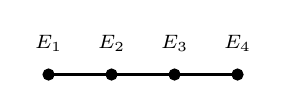
\begin{tikzpicture}[line cap=round,line join=round,x=0.8cm,y=0.8cm]
%\clip(-9,-2.5) rectangle (9,1.);
\draw [line width=1.2pt] (-7.,0.)-- (-4.,0.);
\begin{scriptsize}
\draw [fill=black] (-7,0) circle (2pt);
\draw[color=black] (-7,0.5) node {$E_{1}$};    
\draw [fill=black] (-6,0) circle (2pt);
\draw[color=black] (-6,0.5) node {$E_{2}$};
\draw [fill=black] (-5,0) circle (2pt);
\draw[color=black] (-5,0.5) node {$E_3$};
\draw [fill=black] (-4,0) circle (2pt);
\draw[color=black] (-4,0.5) node {$E_4$};
\end{scriptsize}
\end{tikzpicture}
%\end{figure}
\]
and
\[
%\begin{figure}[h]
\centering
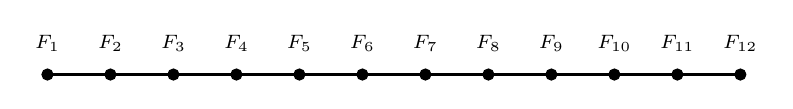
\begin{tikzpicture}[line cap=round,line join=round,x=0.8cm,y=0.8cm]
%\clip(-9,-2.5) rectangle (9,1.);
\draw [line width=1.2pt] (-7.,0.)-- (4.,0.);
\begin{scriptsize}
\draw [fill=black] (-7,0) circle (2pt);
\draw[color=black] (-7,0.5) node {$F_{1}$};    
\draw [fill=black] (-6,0) circle (2pt);
\draw[color=black] (-6,0.5) node {$F_{2}$};
\draw [fill=black] (-5,0) circle (2pt);
\draw[color=black] (-5,0.5) node {$F_3$};
\draw [fill=black] (-4,0) circle (2pt);
\draw[color=black] (-4,0.5) node {$F_4$};
\draw [fill=black] (-3,0) circle (2pt);
\draw[color=black] (-3,0.5) node {$F_5$};
\draw [fill=black] (-2,0) circle (2pt);
\draw[color=black] (-2,0.5) node {$F_6$};
\draw [fill=black] (-1,0) circle (2pt);
\draw[color=black] (-1,0.5) node {$F_7$};
\draw [fill=black] (0,0) circle (2pt);
\draw[color=black] (0,0.5) node {$F_8$};
\draw [fill=black] (1,0) circle (2pt);
\draw[color=black] (1,0.5) node {$F_9$};
\draw [fill=black] (2,0) circle (2pt);
\draw[color=black] (2,0.5) node {$F_{10}$};
\draw [fill=black] (3,0) circle (2pt);
\draw[color=black] (3,0.5) node {$F_{11}$};
\draw [fill=black] (4,0) circle (2pt);
\draw[color=black] (4,0.5) node {$F_{12}$};
\end{scriptsize}
\end{tikzpicture}.
%\end{figure}
\]
Moreover $E:=E_4$ and $F:= F_{12}$ are horizontal curves, namely the birational transforms of the horizontal lines $(1:0:0) \times \PP^1$ and $(0:0:1) \times \PP^1$ under the desingularization morphism $(\lam,\wt \tau): \wt S \to S \subset \PP^2 \times \PP^1$.
The self-intersection numbers are equal to
\begin{align*}
    E_i \cdot E_i &= -2 \quad (i=1,2,3), \quad E \cdot E = -1, \\
    F_i \cdot F_i &= -2 \quad (i = 1,\dots,11), \quad F \cdot F = -1.
\end{align*}
The fibres of the morphism $\wt \tau: \wt S \to \PP^1$ over $(1:0)$ and $(0:1)$ contain the exceptional curves $E_i$ except $E_4 = E$, and $F_i$ except $F_{12}=F$, respectively.
Hence the singular points $P$ and $Q$ on the surface $S$ are rational double points of type $A_3$ and $A_{11}$, respectively.

We denote by $W$, $X$ and $Z$ the birational transforms of the plane projective curves $V(y^4 + xz^3)$, $V(x)$ and $V(z)$ under the morphism $\lam: \wt S \to \PP^2$.
Note that $W$, $X$ and $Z$ are smooth rational curves; indeed the singularity of $V(y^4 + xz^3)$ is resolved by the first blowup over $(1:0:0)$.


The computations also show that the fibre of $\wt \tau$ over the point $(1:0)$ is the Weil divisor
\begin{equation}\label{2024_07_22_13:30}
    \wt \tau^* (1:0) = W + 2 E_1 + 2 E_2 + E_3,
\end{equation}
where the components intersect according to the configuration
\[
%\begin{figure}[h]
\begin{scriptsize}
\begin{tikzpicture}[line cap=round,line join=round,x=0.7cm,y=0.7cm]
%\draw[step=1.0,black,dotted] (-4.5,-4.5) grid (4.5,4.5);
\draw plot [smooth,tension=1] coordinates {(-1.5,-2) (0,0) (-1.5,2)}; \draw (-1.5,2) node[left] {$W$};
\draw (-1.5,0) -- (3,0) node[right] {$E_2$};
\draw (0,-2) -- (0,2) node[above] {$E_1$};
\draw (2,-2) -- (2,2) node[above] {$E_3$};

\end{tikzpicture}
\end{scriptsize}.
%\end{figure}
\]
The intersection matrix of $W$, $E_1$, $E_2$, $E_3$ is equal to
\[ \left( \begin{array}{cccc} 
-6 & 2 & 1 & 0  \\
2 & -2 & 1 & 0 \\
1 & 1 & -2 & 1 \\
0 & 0 & 1 & -2 \\
\end{array} \right) \]
where the self-intersection numbers can be obtained from the property that a fibre meets each of its components with intersection number zero.

The fibre of $\wt \tau$ over the point $(0:1)$ is the Weil divisor
\begin{equation}\label{2024_07_22_13:35}
\begin{aligned}
    \wt \tau^*(0:1) &= 3X + Z + 2 F_1 + 4 F_2 + 6 F_3 + 8 F_4 + 7 F_5 + 6 F_6  \\
    &\qquad + 5 F_7 + 4 F_8 + 3 F_9 + 2 F_{10} + F_{11}
\end{aligned}
\end{equation}
whose components intersect transversely according to the Coxeter-Dynkin diagram
\[
%\begin{figure}[h]
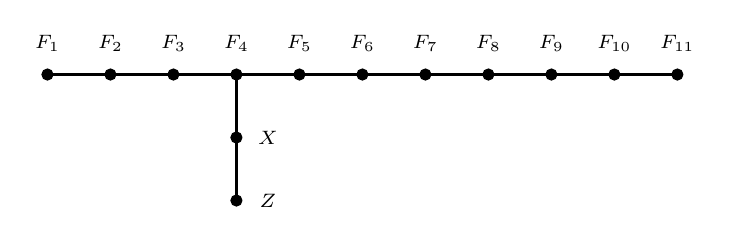
\begin{tikzpicture}[line cap=round,line join=round,x=0.8cm,y=0.8cm]
%\clip(-9,-2.5) rectangle (9,1.);
\draw [line width=1.2pt] (-7.,0.)-- (3.,0.);
\draw [line width=1.2pt] (-4.,0.)-- (-4.,-2.);
\begin{scriptsize}
\draw [fill=black] (-7,0) circle (2pt);
\draw[color=black] (-7,0.5) node {$F_{1}$};    
\draw [fill=black] (-6,0) circle (2pt);
\draw[color=black] (-6,0.5) node {$F_{2}$};
\draw [fill=black] (-5,0) circle (2pt);
\draw[color=black] (-5,0.5) node {$F_3$};
\draw [fill=black] (-4,0) circle (2pt);
\draw[color=black] (-4,0.5) node {$F_4$};
\draw [fill=black] (-4,-1.) circle (2pt);
\draw[color=black] (-4.5 + 1,-1) node {$X$};
\draw [fill=black] (-4.,-2.) circle (2pt);
\draw[color=black] (-4.5 + 1,-2) node {$Z$};
\draw [fill=black] (-3,0) circle (2pt);
\draw[color=black] (-3,0.5) node {$F_5$};
\draw [fill=black] (-2.,0.) circle (2pt);
\draw[color=black] (-2.,.5) node {$F_6$};
\draw [fill=black] (-1.,0.) circle (2pt);
\draw[color=black] (-1.,.5) node {$F_7$};
\draw [fill=black] (0.,0.) circle (2pt);
\draw[color=black] (0.,.5) node {$F_8$};
\draw [fill=black] (1.,0.) circle (2pt);
\draw[color=black] (1.,0.5) node {$F_9$};
\draw [fill=black] (2.,0.) circle (2pt);
\draw[color=black] (2.,.5) node {$F_{10}$};
\draw [fill=black] (3.,0.) circle (2pt);
\draw[color=black] (3.,0.5) node {$F_{11}$};
\end{scriptsize}
\end{tikzpicture}
%\end{figure}
\]
Moreover $X\cdot X = Z \cdot Z = -3$.
Note also that $W \cdot F = Z \cdot E = 1$.

To summarize we put the curves appearing in the discussion of the bad fibres $\wt \tau^*(1:0)$ and $\wt \tau^*(0:1)$ into a unique configuration in Figure~\ref{2024_07_23_20:15}.
\begin{figure}[h]

\centering
\begin{tikzpicture}[line cap=round,line join=round,x=0.7cm,y=0.7cm]
%\clip(-9,-2.5) rectangle (9,1.);

\begin{scriptsize}

%%%%%%%%%%%%%%%%%%%%%%%%%%%%%%%%%%%%%%%%%%%%%%%%%%%%%%%%%%%%
%% diagram above
%%%%%%%%%%%%%%%%%%%%%%%%%%%%%%%%%%%%%%%%%%%%%%%%%%%%%%%%%%%%

%vertical lines above
\draw (-6,0 - .6) -- (-6,2 + .6) ;  \draw[color=black] (-6,2 + .6) node[above] {$F_{11}$}; 
\draw (-4,0 - .6) -- (-4,2 + .6) ;  \draw[color=black] (-4,2 + .6) node[above] {$F_9$}; 
\draw (-2,0 - .6) -- (-2,2 + .6) ;  \draw[color=black] (-2,2 + .6) node[above] {$F_7$}; 
\draw (0,0 - .6) -- (0,2 + .6) ;  \draw[color=black] (0,2 + .6) node[above] {$F_5$}; 
\draw (2,0 - .6) -- (2,2 + .6) ;  \draw[color=black] (2,2 + .6) node[above] {$F_3$}; 
\draw (4,0 - .6) -- (4,2 + .6) ;  \draw[color=black] (4,2 + .6) node[above] {$F_1$}; 

%horizontal lines above 
\draw (-6- .6,2) -- (-4 + .6,2) ; \draw[color=black] (-5,2 + .0) node[above] {$F_{10}$}; 
\draw (-4- .6,0) -- (-2 + .6,0) ;  \draw[color=black] (-3,0 + .0) node[above] {$F_8$}; 
\draw (-2- .6,2) -- (0 + .6,2) ;  \draw[color=black] (-1,2 + .0) node[above] {$F_6$}; 
\draw (0- .6,0) -- (2 + .6,0) ;  \draw[color=black] (2 + .6,0) node[right] {$F_4$};
\draw (2- .6,2) -- (4 + .6,2) ;  \draw[color=black] (3,2 + .0) node[above] {$F_2$}; 

% "new lines" above
\draw (1,0.5) -- (2.5,-2); \draw[color=black] (1,0.5) node[above] {$X$};
\draw (1.5,-1.5) -- (6.1,-1.5); \draw[color=black] (6.1,-1.5) node[right] {$Z$}; 

%curves above
%\draw plot [smooth,tension=1] coordinates {(.9,.5) (1.6,-.5-.3) (3,-1)}; \draw (.9,.5) node[above] {$X$};
%\draw plot [smooth,tension=1] coordinates {(2.3,-.5) (3,-1.9) (4.5,-2.5)}; \draw (3,-1.9) node[left] {$L$};
%\draw plot [smooth,tension=1] coordinates {(3.7,-2) (4.7,-3.1) (6,-3.5)}; \draw (6,-3.5) node[right] {$Z$};

%lines/curves below
\draw (-5 +3,-5 - .6) -- (-5 +3,-3 + .6) ; \draw[color=black] (-5 +3,-5 - .6) node[below] {$E_1$}; 
\draw (-2 +3,-5 - .6) -- (-2 +3,-3 + .6) ; \draw[color=black] (-2 +3,-5 - .6) node[below] {$E_3$}; 
\draw (-5- .6 +3,-4) -- (-2 + .6 +3,-4) ;  \draw[color=black] (-5 +3 + 1.5,-4) node[above] {$E_2$};
\draw plot [smooth,tension=1] coordinates {(-2 -5 +3,-1.5 -4) (0-5 +3,0-4) (-2 -5 +3,1.5 -4)}; \draw (-2 -5 +3,-1.5 -4) node[left] {$W$};

%"horizontal" curves linking above and below
\draw (-6 - .6/2,0 + .6) -- (-3 - .2/2,-6 + .2); \draw[color=black] (-4.5,-3) node[left] {$F$}; 
%\draw (1 - .6,-5 - .6*2/5) -- (6,-3); \draw[color=black] (3.5,-4) node[below] {$E$}; 
\draw (1 - .6,-5 - .6*4/5) -- (6,-1); \draw[color=black] (3.5,-3) node[below] {$E$};


%%%%%%%%%%%%%%%%%%%%%%%%%%%%%%%%%%%%%%%%%%%%%%%%%%%%%%%%%%%%
%% diagram below
%%%%%%%%%%%%%%%%%%%%%%%%%%%%%%%%%%%%%%%%%%%%%%%%%%%%%%%%%%%%
\begin{comment}

%first group of lines above
\draw (-8 -.6 +2,-4 + .6/2 -6) -- (-6 + .6 +2,-5 - .6/2 -6) ;  \draw[color=black] (-5,-10.5) node[above] {$F_6'$};
\draw (-4 -.6 +2,-4 + .6/2 -6) -- (-2 + .6 +2,-5 - .6/2 -6) ;  \draw[color=black] (-1,-10.5) node[above] {$F_4'$};
\draw (0 -.6 +2,-4 + .6/2 -6) -- (2 + .6 +2,-5 - .6/2 -6) ;  \draw[color=black] (3 + .3,-10.5 - .3/2 + .1) node[above] {$X'$};

%second group of lines above
\draw (-4 + .6 +2,-4 + .6/2 -6) -- (-6 - .6 +2,-5 - .6/2 -6) ;  \draw[color=black] (-3 + .3,-10.5 + .3/2) node[below] {$F_5'$}; 
\draw (0 + .6 +2,-4 + .6/2 -6) -- (-2 - .6 +2,-5 - .6/2 -6) ;  \draw[color=black] (-2 - .6 +2,-5 - .6/2 -6) node[left] {$F_3'$}; 

%"new lines" above
\draw (1,-9.5) -- (1.5,-12); \draw (1,-9.5) node[above] {$F_2'$};
\draw (1,-11.4) -- (3.5,-12.6); \draw (2.8,-11.7) node[left] {$F_1'$};
\draw (2.5,-12.4) -- (6 + .1,-12.4); \draw[color=black] (6 + .1,-12.4) node[right] {$Z'$};

%curves above
%\draw plot [smooth,tension=1] coordinates {(.9,.5-4 -6) (1.6,-.5-.3-4 -6) (3,-1-4 -6)}; \draw (.9,.5-4 -6) node[above] {$F_2'$};
%\draw plot [smooth,tension=1] coordinates {(2.3,-.5-4 -6) (3,-1.9-4 -6) (4.5,-2.5-4 -6)}; \draw (3-.1,-1.9-4 -6) node[left] {$F_1'$};
%\draw plot [smooth,tension=1] coordinates {(3.7,-2-4 -6) (4.7,-3.1-4 -6) (6,-3.5-4 -6)}; \draw (6,-3.5-4 -6) node[right] {$Z'$};

%line below
\draw (-2 -.6 ,-14 + .6/3) -- (1 + .6,-15 - .6/3) ;  \draw[color=black] (-.5,-14.5) node[above] {$E_1'$};
%points below
\draw [fill=black] (-2,-14) circle (1.6pt);
\draw [fill=black] (1,-15) circle (1.6pt);

%curve below
\draw plot [smooth,tension=1] coordinates {(-4,-15) (-2,-14) (0 -1.5,-16+.4)}; \draw (-4,-15) node[left] {$W'$};

%points above
\draw [fill=black] (-8 +2,-4 -6) circle (1.6pt);
\draw [fill=black] (-6 +2,-5 -6) circle (1.6pt);
\draw [fill=black] (-4 +2,-4 -6) circle (1.6pt);
\draw [fill=black] (-2 +2,-5 -6) circle (1.6pt);
\draw [fill=black] (0 +2.,-4 -6) circle (1.6pt);
\draw [fill=black] (2 +2,-5 -6) circle (1.6pt);


%"horizontal" curves linking above and below
\draw (-6 - .6*3/5,-10 + .6) -- (-3,-15); \draw[color=black] (-4.5,-12.5) node[left] {$F'$};
%\draw (1 - .6,-15 - .6*2/5) -- (6,-13); \draw[color=black] (3.5,-14) node[below] {$E'$};
\draw (1 - .5,-15 - .5*3/5) -- (6,-12); \draw[color=black] (3.5,-13.5) node[below] {$E'$};

\end{comment}

\end{scriptsize}
\end{tikzpicture}
\caption{Configuration of curves on $\wt S$}\label{2024_07_23_20:15}
\end{figure}

The remaining fibres of $\wt \tau$ are integral curves of self-intersection number zero.
As the fibres of $\wt \tau$ do not contain curves of self-intersection $-1$, that is, curves that are contractible according to Castelnuovo's contractibility criterion, we deduce that the fibration $\wt \tau: \wt S \to \PP^1$ is a relatively minimal model and hence by a theorem of Lichtenbaum--Shafarevich (see \cite[Theorem~4.4]{Lic68}, \cite[p.\,155]{Sha66}, or \cite[p.\,422]{Liu02}) the (unique) minimal model of the function field $F|K = k(S)|k(\PP^1)$.
However, as the two horizontal curves $E=E_4$ and $F=F_{12}$ are contractible, the smooth surface $\wt S$ is not relatively minimal over $\Spec(k)$.

Since the Frobenius pullback $F_1|K$ of the function field $F|K = k(\wt S)|k(\PP^1)$ is quasi-elliptic, it follows that the fibration $\wt \tau: \wt S \to \PP^1$ is an inseparable covering of degree two of a quasi-elliptic fibration.
In the remaining of this section we describe this covering.


Let $S' \su \PP^2 \times \PP^1$ be the integral projective algebraic surface of the pairs $((u:v:w),(t_0:t_1))$ satisfying the bihomogeneous equation
\[ t_0 (u v^2 + w^3) + t_1 u^2 w = 0. \]
This defines a pencil of plane projective cubic curves, whose base points are equal to $(1:0:0)$ and $(0:1:0)$.
The members of this pencil are up to isomorphisms the fibres of the second projection morphism $S\to \PP^1$.
These fibres are cuspidal cubic curves, except the fibre over the point $(0:1)$, which consists of the line $V(w)$ and the double line $V(u^2)$.

The surface $S' \su \PP^2 \times \PP^1$ has precisely two singularities at the points $P' = ((1:0:0),(1:0))$ and $Q'=((0:1:0),(0:1))$.
The first projection $S' \to \PP^2$ is a birational morphism, whose inverse is the rational map
\[ (\mathrm{id},\tau'):\PP^2 \ttto S' \subset \PP^2 \times \PP^1 \]
where $\tau':\PP^2 \ttto \PP^1$, $(u:v:w) \mapsto (u^2 w: uv^2 + w^3)$, is undefined only at the base points $(1:0:0)$ and $(0:1:0)$.
Resolving the indeterminacy of $\tau'$ we obtain the commutative diagram
\[
\begin{tikzcd}
    \wt S' \ar[d,"\lam'"] \ar[dr,"\wt \tau'", bend left=20] \\
    \PP^2 \ar[r,dashed,"\tau'"] & \PP^1
\end{tikzcd}
\]
where $\wt S'$ is a smooth integral projective surface and where $\lam'$ and $\wt \tau'$ are morphisms, which provide a desingularization morphism
\[ (\lam',\wt \tau') : \wt S' \tto S' \subset \PP^2 \times \PP^1 \]
of the variety $S'$.
The morphism $\lam':\wt S' \to \PP^2$ is obtained by a chain of 2 blowups over $(1:0:0)$ and $7$ blowups over $(0:1:0)$.
The corresponding exceptional curves $E_i'$ ($i=1,2$) and $F_i'$ ($i=1,\dots,7$) on $\wt S'$ intersect according to the Dynkin diagrams $A_2$ and $A_7$, respectively.
Moreover, $E':= E_2'$ and $F':= F_7'$ are horizontal curves of self-intersection number $-1$, namely the birational transforms of the horizontal lines $(1:0:0)\times \PP^1$ and $(0:1:0)\times \PP^1$ under the desingularization morphism $\wt S' \to S'$.
The singular points $P'$ and $Q'$ on the surface $S'$ are rational double points of type $A_1$ and $A_6$, respectively.

We denote by $W'$, $X'$ and $Z'$ the birational transforms of the plane projective curves $V(uv^2 + w^3)$, $V(u)$ and $V(w)$.
The fibres of the morphism $\wt \tau' : \wt S' \to \PP^1$ over the points $(1:0)$ and $(0:1)$ are of type $\wt A_1^*$ and $\wt E_7$ respectively (see \cite[Theorem~4.1.4 and Corollary~4.3.22]{CDL23}).
More precisely, these fibres are given by
\[ \wt \tau'^* (1:0) = W' + E_1' \]
where $W'$ and $E_1'$ meet with intersection number $2$ at only one point, and
\[ \wt \tau'^*(0:1) = 2 X' + Z' + 2 F'_1 + 3 F'_2 + 4 F'_3 + 3 F'_4 + 2 F'_5 + F'_6  \]
where the components intersect transversely according to the diagram
\[
%\begin{figure}[h]
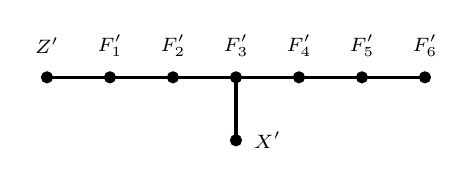
\begin{tikzpicture}[line cap=round,line join=round,x=0.8cm,y=0.8cm]
%\clip(-9,-2.5) rectangle (9,1.);
\draw [line width=1.2pt] (-7.,0.)-- (-1.,0.);
\draw [line width=1.2pt] (-4.,0.)-- (-4.,-1.);
\begin{scriptsize}
\draw [fill=black] (-7,0) circle (2pt);
\draw[color=black] (-7,0.5) node {$Z'$};    
\draw [fill=black] (-6,0) circle (2pt);
\draw[color=black] (-6,0.5) node {$F_1'$};
\draw [fill=black] (-5,0) circle (2pt);
\draw[color=black] (-5,0.5) node {$F_2'$};
\draw [fill=black] (-4,0) circle (2pt);
\draw[color=black] (-4,0.5) node {$F_3'$};
\draw [fill=black] (-4,-1.) circle (2pt);
\draw[color=black] (-4.5 + 1,-1) node {$X'$};
\draw [fill=black] (-3,0) circle (2pt);
\draw[color=black] (-3,0.5) node {$F_4'$};
\draw [fill=black] (-2.,0.) circle (2pt);
\draw[color=black] (-2.,.5) node {$F_5'$};
\draw [fill=black] (-1.,0.) circle (2pt);
\draw[color=black] (-1.,.5) node {$F_6'$};
\end{scriptsize}
\end{tikzpicture}
%\end{figure}
\]
The self-intersection numbers of the curves $E_1',F_1',\dots,F_5',W',X',Z'$ are equal to $-2$.
The remaining fibres of $\wt \tau'$ are integral curves of self-intersection number zero.
Thus the fibration $\wt S' \to \PP^1$ is the minimal model of the Frobenius pullback $F_1|K$ of the function field $F|K$.





\begin{figure}[h]

\centering
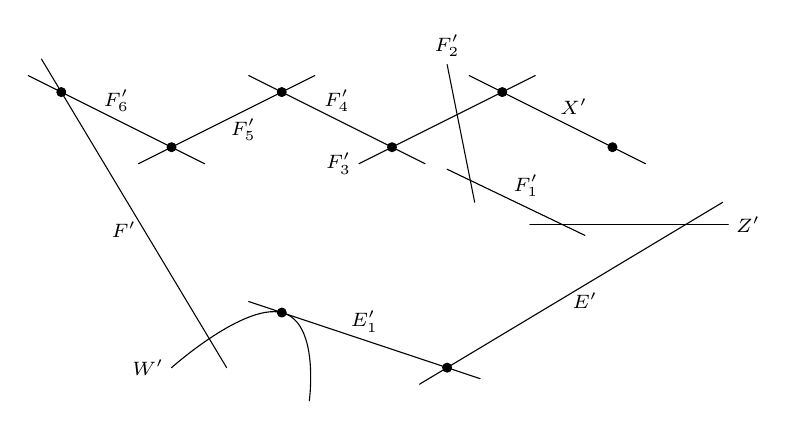
\begin{tikzpicture}[line cap=round,line join=round,x=0.7cm,y=0.7cm]
%\clip(-9,-2.5) rectangle (9,1.);

\begin{scriptsize}

%%%%%%%%%%%%%%%%%%%%%%%%%%%%%%%%%%%%%%%%%%%%%%%%%%%%%%%%%%%%
%% diagram above
%%%%%%%%%%%%%%%%%%%%%%%%%%%%%%%%%%%%%%%%%%%%%%%%%%%%%%%%%%%%

\begin{comment}
%vertical lines above
\draw (-6,0 - .6) -- (-6,2 + .6) ;  \draw[color=black] (-6,2 + .6) node[above] {$F_{11}$}; 
\draw (-4,0 - .6) -- (-4,2 + .6) ;  \draw[color=black] (-4,2 + .6) node[above] {$F_9$}; 
\draw (-2,0 - .6) -- (-2,2 + .6) ;  \draw[color=black] (-2,2 + .6) node[above] {$F_7$}; 
\draw (0,0 - .6) -- (0,2 + .6) ;  \draw[color=black] (0,2 + .6) node[above] {$F_5$}; 
\draw (2,0 - .6) -- (2,2 + .6) ;  \draw[color=black] (2,2 + .6) node[above] {$F_3$}; 
\draw (4,0 - .6) -- (4,2 + .6) ;  \draw[color=black] (4,2 + .6) node[above] {$F_1$}; 

%horizontal lines above 
\draw (-6- .6,2) -- (-4 + .6,2) ; \draw[color=black] (-5,2 + .0) node[above] {$F_{10}$}; 
\draw (-4- .6,0) -- (-2 + .6,0) ;  \draw[color=black] (-3,0 + .0) node[above] {$F_8$}; 
\draw (-2- .6,2) -- (0 + .6,2) ;  \draw[color=black] (-1,2 + .0) node[above] {$F_6$}; 
\draw (0- .6,0) -- (2 + .6,0) ;  \draw[color=black] (2 + .6,0) node[right] {$F_4$};
\draw (2- .6,2) -- (4 + .6,2) ;  \draw[color=black] (3,2 + .0) node[above] {$F_2$}; 

% "new lines" above
\draw (1,0.5) -- (2.5,-2); \draw[color=black] (1,0.5) node[above] {$X$};
\draw (1.5,-1.5) -- (6.1,-1.5); \draw[color=black] (6.1,-1.5) node[right] {$Z$}; 

%curves above
%\draw plot [smooth,tension=1] coordinates {(.9,.5) (1.6,-.5-.3) (3,-1)}; \draw (.9,.5) node[above] {$X$};
%\draw plot [smooth,tension=1] coordinates {(2.3,-.5) (3,-1.9) (4.5,-2.5)}; \draw (3,-1.9) node[left] {$L$};
%\draw plot [smooth,tension=1] coordinates {(3.7,-2) (4.7,-3.1) (6,-3.5)}; \draw (6,-3.5) node[right] {$Z$};

%lines/curves below
\draw (-5 +3,-5 - .6) -- (-5 +3,-3 + .6) ; \draw[color=black] (-5 +3,-5 - .6) node[below] {$E_1$}; 
\draw (-2 +3,-5 - .6) -- (-2 +3,-3 + .6) ; \draw[color=black] (-2 +3,-5 - .6) node[below] {$E_3$}; 
\draw (-5- .6 +3,-4) -- (-2 + .6 +3,-4) ;  \draw[color=black] (-5 +3 + 1.5,-4) node[above] {$E_2$};
\draw plot [smooth,tension=1] coordinates {(-2 -5 +3,-1.5 -4) (0-5 +3,0-4) (-2 -5 +3,1.5 -4)}; \draw (-2 -5 +3,-1.5 -4) node[left] {$W$};

%"horizontal" curves linking above and below
\draw (-6 - .6/2,0 + .6) -- (-3 - .2/2,-6 + .2); \draw[color=black] (-4.5,-3) node[left] {$F$}; 
%\draw (1 - .6,-5 - .6*2/5) -- (6,-3); \draw[color=black] (3.5,-4) node[below] {$E$}; 
\draw (1 - .6,-5 - .6*4/5) -- (6,-1); \draw[color=black] (3.5,-3) node[below] {$E$};

\end{comment}

%%%%%%%%%%%%%%%%%%%%%%%%%%%%%%%%%%%%%%%%%%%%%%%%%%%%%%%%%%%%
%% diagram below
%%%%%%%%%%%%%%%%%%%%%%%%%%%%%%%%%%%%%%%%%%%%%%%%%%%%%%%%%%%%


%first group of lines above
\draw (-8 -.6 +2,-4 + .6/2 -6) -- (-6 + .6 +2,-5 - .6/2 -6) ;  \draw[color=black] (-5,-10.5) node[above] {$F_6'$};
\draw (-4 -.6 +2,-4 + .6/2 -6) -- (-2 + .6 +2,-5 - .6/2 -6) ;  \draw[color=black] (-1,-10.5) node[above] {$F_4'$};
\draw (0 -.6 +2,-4 + .6/2 -6) -- (2 + .6 +2,-5 - .6/2 -6) ;  \draw[color=black] (3 + .3,-10.5 - .3/2 + .1) node[above] {$X'$};

%second group of lines above
\draw (-4 + .6 +2,-4 + .6/2 -6) -- (-6 - .6 +2,-5 - .6/2 -6) ;  \draw[color=black] (-3 + .3,-10.5 + .3/2) node[below] {$F_5'$}; 
\draw (0 + .6 +2,-4 + .6/2 -6) -- (-2 - .6 +2,-5 - .6/2 -6) ;  \draw[color=black] (-2 - .6 +2,-5 - .6/2 -6) node[left] {$F_3'$}; 

%"new lines" above
\draw (1,-9.5) -- (1.5,-12); \draw (1,-9.5) node[above] {$F_2'$};
\draw (1,-11.4) -- (3.5,-12.6); \draw (2.8,-11.7) node[left] {$F_1'$};
\draw (2.5,-12.4) -- (6 + .1,-12.4); \draw[color=black] (6 + .1,-12.4) node[right] {$Z'$};

%curves above
%\draw plot [smooth,tension=1] coordinates {(.9,.5-4 -6) (1.6,-.5-.3-4 -6) (3,-1-4 -6)}; \draw (.9,.5-4 -6) node[above] {$F_2'$};
%\draw plot [smooth,tension=1] coordinates {(2.3,-.5-4 -6) (3,-1.9-4 -6) (4.5,-2.5-4 -6)}; \draw (3-.1,-1.9-4 -6) node[left] {$F_1'$};
%\draw plot [smooth,tension=1] coordinates {(3.7,-2-4 -6) (4.7,-3.1-4 -6) (6,-3.5-4 -6)}; \draw (6,-3.5-4 -6) node[right] {$Z'$};

%line below
\draw (-2 -.6 ,-14 + .6/3) -- (1 + .6,-15 - .6/3) ;  \draw[color=black] (-.5,-14.5) node[above] {$E_1'$};
%points below
\draw [fill=black] (-2,-14) circle (1.6pt);
\draw [fill=black] (1,-15) circle (1.6pt);

%curve below
\draw plot [smooth,tension=1] coordinates {(-4,-15) (-2,-14) (0 -1.5,-16+.4)}; \draw (-4,-15) node[left] {$W'$};

%points above
\draw [fill=black] (-8 +2,-4 -6) circle (1.6pt);
\draw [fill=black] (-6 +2,-5 -6) circle (1.6pt);
\draw [fill=black] (-4 +2,-4 -6) circle (1.6pt);
\draw [fill=black] (-2 +2,-5 -6) circle (1.6pt);
\draw [fill=black] (0 +2.,-4 -6) circle (1.6pt);
\draw [fill=black] (2 +2,-5 -6) circle (1.6pt);


%"horizontal" curves linking above and below
\draw (-6 - .6*3/5,-10 + .6) -- (-3,-15); \draw[color=black] (-4.5,-12.5) node[left] {$F'$};
%\draw (1 - .6,-15 - .6*2/5) -- (6,-13); \draw[color=black] (3.5,-14) node[below] {$E'$};
\draw (1 - .5,-15 - .5*3/5) -- (6,-12); \draw[color=black] (3.5,-13.5) node[below] {$E'$};



\end{scriptsize}
\end{tikzpicture}
\caption{Configuration of curves on $\wt S'$}\label{2024_07_23_20:20}
\end{figure}

We finally explain how the fibration $f:\wt S\to \PP^1$ covers the quasi-elliptic fibration $f':\wt S'\to \PP^1$. To this end we consider the commutative diagram
\[
\begin{tikzcd}
    S \ar[d,dashed] \ar[r] & \PP^2 \ar[d,dashed] \\
    S' \ar[r] & \PP^2 
\end{tikzcd}
\]
where the dashed arrows represent the rational maps
\[ ((x:y:z),(t_0:t_1)) \mapsto ((x^2:y^2:xz),(t_0:t_1)) \quad \text{and} \quad (x:y:z)\mapsto (x^2 : y^2 : xz). \]
These maps are undefined only at the points $Q\in S$ and $(0:0:1)\in \PP^2$ respectively.
We analyse how the corresponding rational map
\[ \wt S \ttto \wt S' \]
transforms the fibres over $\PP^1$.
The fibres of $\wt \tau: \wt S \to \PP^1$ over the points different from $(1:0)$ and $(0:1)$ are applied to the corresponding fibres of $\wt \tau' : \wt S' \to \PP^1$ by the quadratic transformation $(x:y:z)\mapsto (x^2 : y^2 : xz)$.
The exceptional curves $E_1$, $E_3$, $F_1$, $F_3$, $F_5$, $F_7$, $F_9$, $F_{11}$ with odd indices are contracted to points,
the exceptional curves $E_2$, $E=E_4$, $F_2$, $F_4$, $F_6$, $F_8$, $F_{10}$, $F=F_{12}$ with even indices are mapped isomorphically onto the curves $E_1'$, $E'=E_2'$, $X'$, $F_3'$, $F_4'$, $F_5'$, $F_6'$, $F'=F_7'$, 
and the curves $X$, $Z$ and $W$ are mapped onto the curves $F_2'$, $Z'$ and $W'$ by inseparable morphisms of degree two.
However, the curve $F_1' \subset \wt S'$ is not covered by any curve on $S$, and so the rational map $\wt S \ttto \wt S'$ is not a morphism.
More precisely, the rational map $\wt S \ttto \wt S'$ is undefined only at the intersection point of $X$ and $Z$. This indeterminacy can be resolved by a unique blowup, whose exceptional line is mapped isomorphically onto the curve $F_1'$.



\begin{bibdiv}
\begin{biblist}%*{labels={numeric}}
\bib{BedSt87}{article}{
  author={Bedoya, Hernando},
  author={St\"ohr, Karl-Otto},
  title={An algorithm to calculate discrete invariants of singular primes in function fields},
  journal={J. Number Theory},
  volume={27},
  date={1987},
  number={3},
  pages={310--323},
}

\bib{BM76}{article}{
  author={Bombieri, Enrico},
  author={Mumford, David},
  title={Enriques' classification of surfaces in char. $p$. III},
  journal={Invent. Math.},
  volume={35},
  date={1976},
  pages={197--232},
}

\bib{BM77}{article}{
  author={Bombieri, Enrico},
  author={Mumford, David},
  title={Enriques' classification of surfaces in char. $p$. II},
  book={ title={Complex Analysis and Algebraic Geometry}, editor={W. L. Baily}, editor={T. Shioda}, publisher={Iwanami Shoten, Tokyo}, },
  date={1977},
  pages={23--42},
}

\bib{CDL23}{book}{
  author={Cossec, François},
  author={Dolgachev, Igor},
  author={Liedtke, Christian},
  title={Enriques Surfaces I},
  publisher={Springer Nature Singapore},
  date={2025},
  pages={xxi+681 pp.},
}

\bib{JVV24}{article}{
  author={Frei, Sarah},
  author={Ji, Lena},
  author={Sankar, Soumya},
  author={Viray, Bianca},
  author={Vogt, Isabel},
  title={Curve classes on conic bundle threefolds and applications to rationality},
  journal={Algebr. Geom.},
  volume={11},
  date={2024},
  number={3},
  pages={421--459},
}

\bib{HiSt22}{article}{
  author={Hilario, Cesar},
  author={St\"ohr, Karl-Otto},
  title={On regular but non-smooth integral curves},
  journal={J. Algebra},
  volume={661},
  date={2025},
  pages={278--300},
}

\bib{HiSt23}{article}{
  author={Hilario, Cesar},
  author={St\"ohr, Karl-Otto},
  title={Fibrations by plane quartic curves with a canonical moving singularity},
  journal={J. Pure Appl. Algebra},
  volume={229},
  date={2025},
  number={4},
  pages={Paper No. 107918, 24},
}

\bib{Kod63}{article}{
  author={Kodaira, Kunihiko},
  title={On compact analytic surfaces. II, III},
  journal={Ann. of Math. (2)},
  volume={77},
  date={1963},
  pages={563--626; {\bf 78} (1963), 1--40},
}

\bib{Lan79}{article}{
  author={Lang, William E.},
  title={Quasi-elliptic surfaces in characteristic three},
  journal={Ann. Sci. \'Ecole Norm. Sup. (4)},
  volume={12},
  date={1979},
  number={4},
  pages={473--500},
}

\bib{Lic68}{article}{
  author={Lichtenbaum, Stephen},
  title={Curves over discrete valuation rings},
  journal={Amer. J. Math.},
  volume={90},
  date={1968},
  pages={380--405},
}

\bib{Lied13}{article}{
  author={Liedtke, Christian},
  title={Algebraic surfaces in positive characteristic},
  conference={ title={Birational geometry, rational curves, and arithmetic}, },
  book={ series={Simons Symp.}, publisher={Springer, Cham}, },
  date={2013},
  pages={229--292},
}

\bib{Liu02}{book}{
  author={Liu, Qing},
  title={Algebraic geometry and arithmetic curves},
  series={Oxford Graduate Texts in Mathematics},
  volume={6},
  publisher={Oxford University Press, Oxford},
  date={2002},
  pages={xvi+576 pp.},
}

\bib{Ner64}{article}{
  author={N\'eron, Andr\'e},
  title={Mod\`eles minimaux des vari\'et\'es ab\'eliennes sur les corps locaux et globaux},
  journal={Inst. Hautes \'Etudes Sci. Publ. Math.},
  date={1964},
  number={21},
  pages={128 pp.},
}

\bib{Pro18}{article}{
  author={Prokhorov, Yuri},
  title={The rationality problem for conic bundles},
  journal={Russian Math. Surveys},
  volume={73},
  date={2018},
  number={3},
  pages={375--456},
}

\bib{Sal11}{article}{
  author={Salom\~ao, Rodrigo},
  title={Fibrations by nonsmooth genus three curves in characteristic three},
  journal={J. Pure Appl. Algebra},
  volume={215},
  date={2011},
  number={8},
  pages={1967--1979},
}

\bib{Sal14}{article}{
  author={Salom\~ao, Rodrigo},
  title={Fibrations by curves with more than one nonsmooth point},
  journal={Bull. Braz. Math. Soc. (N.S.)},
  volume={45},
  date={2014},
  number={2},
  pages={267--292},
}

\bib{Sc09}{article}{
  author={Schr\"oer, Stefan},
  title={On genus change in algebraic curves over imperfect fields},
  journal={Proc. Amer. Math. Soc.},
  volume={137},
  date={2009},
  number={4},
  pages={1239-1243},
}

\bib{SchSh10}{article}{
  author={Sch\"{u}tt, Matthias},
  author={Shioda, Tetsuji},
  title={Elliptic surfaces},
  conference={ title={Algebraic geometry in East Asia -- Seoul 2008}, },
  book={ series={Adv. Stud. Pure Math.}, volume={60}, publisher={Math. Soc. Japan, Tokyo}, },
  date={2010},
  pages={51--160},
}

\bib{Shaf13a}{book}{
  author={Shafarevich, Igor R.},
  title={Basic Algebraic Geometry 1},
  edition={3},
  publisher={Springer, Heidelberg},
  date={2013},
  pages={xviii+310 pp.},
}

\bib{Sha66}{book}{
  author={Shafarevich, Igor R.},
  title={Lectures on minimal models and birational transformations of two dimensional schemes},
  series={Tata Institute of Fundamental Research Lectures on Mathematics and Physics},
  volume={37},
  note={Notes by C. P. Ramanujam},
  publisher={Tata Institute of Fundamental Research, Bombay},
  date={1966},
  pages={iv+175 pp.},
}

\bib{St04}{article}{
  author={St\"ohr, Karl-Otto},
  title={On Bertini's theorem in characteristic $p$ for families of canonical curves in $\PP ^{(p-3)/2}$},
  journal={Proc. London Math. Soc. (3)},
  volume={89},
  date={2004},
  number={2},
  pages={291--316},
}

\bib{Tate52}{article}{
  author={Tate, John},
  title={Genus change in inseparable extensions of function fields},
  journal={Proc. Amer. Math. Soc.},
  volume={3},
  date={1952},
  pages={400--406},
}
\end{biblist}
\end{bibdiv}

\end{document}
